% Options for packages loaded elsewhere
% Options for packages loaded elsewhere
\PassOptionsToPackage{unicode}{hyperref}
\PassOptionsToPackage{hyphens}{url}
%
\documentclass[
  11pt,
  letterpaper,
]{book}
\usepackage{xcolor}
\usepackage[margin=2.5cm,paper=a4paper]{geometry}
\usepackage{amsmath,amssymb}
\setcounter{secnumdepth}{-\maxdimen} % remove section numbering
\usepackage{iftex}
\ifPDFTeX
  \usepackage[T1]{fontenc}
  \usepackage[utf8]{inputenc}
  \usepackage{textcomp} % provide euro and other symbols
\else % if luatex or xetex
  \usepackage{unicode-math} % this also loads fontspec
  \defaultfontfeatures{Scale=MatchLowercase}
  \defaultfontfeatures[\rmfamily]{Ligatures=TeX,Scale=1}
\fi
\usepackage{lmodern}
\ifPDFTeX\else
  % xetex/luatex font selection
\fi
% Use upquote if available, for straight quotes in verbatim environments
\IfFileExists{upquote.sty}{\usepackage{upquote}}{}
\IfFileExists{microtype.sty}{% use microtype if available
  \usepackage[]{microtype}
  \UseMicrotypeSet[protrusion]{basicmath} % disable protrusion for tt fonts
}{}
\makeatletter
\@ifundefined{KOMAClassName}{% if non-KOMA class
  \IfFileExists{parskip.sty}{%
    \usepackage{parskip}
  }{% else
    \setlength{\parindent}{0pt}
    \setlength{\parskip}{6pt plus 2pt minus 1pt}}
}{% if KOMA class
  \KOMAoptions{parskip=half}}
\makeatother
% Make \paragraph and \subparagraph free-standing
\makeatletter
\ifx\paragraph\undefined\else
  \let\oldparagraph\paragraph
  \renewcommand{\paragraph}{
    \@ifstar
      \xxxParagraphStar
      \xxxParagraphNoStar
  }
  \newcommand{\xxxParagraphStar}[1]{\oldparagraph*{#1}\mbox{}}
  \newcommand{\xxxParagraphNoStar}[1]{\oldparagraph{#1}\mbox{}}
\fi
\ifx\subparagraph\undefined\else
  \let\oldsubparagraph\subparagraph
  \renewcommand{\subparagraph}{
    \@ifstar
      \xxxSubParagraphStar
      \xxxSubParagraphNoStar
  }
  \newcommand{\xxxSubParagraphStar}[1]{\oldsubparagraph*{#1}\mbox{}}
  \newcommand{\xxxSubParagraphNoStar}[1]{\oldsubparagraph{#1}\mbox{}}
\fi
\makeatother

\usepackage{color}
\usepackage{fancyvrb}
\newcommand{\VerbBar}{|}
\newcommand{\VERB}{\Verb[commandchars=\\\{\}]}
\DefineVerbatimEnvironment{Highlighting}{Verbatim}{commandchars=\\\{\}}
% Add ',fontsize=\small' for more characters per line
\usepackage{framed}
\definecolor{shadecolor}{RGB}{241,243,245}
\newenvironment{Shaded}{\begin{snugshade}}{\end{snugshade}}
\newcommand{\AlertTok}[1]{\textcolor[rgb]{0.68,0.00,0.00}{#1}}
\newcommand{\AnnotationTok}[1]{\textcolor[rgb]{0.37,0.37,0.37}{#1}}
\newcommand{\AttributeTok}[1]{\textcolor[rgb]{0.40,0.45,0.13}{#1}}
\newcommand{\BaseNTok}[1]{\textcolor[rgb]{0.68,0.00,0.00}{#1}}
\newcommand{\BuiltInTok}[1]{\textcolor[rgb]{0.00,0.23,0.31}{#1}}
\newcommand{\CharTok}[1]{\textcolor[rgb]{0.13,0.47,0.30}{#1}}
\newcommand{\CommentTok}[1]{\textcolor[rgb]{0.37,0.37,0.37}{#1}}
\newcommand{\CommentVarTok}[1]{\textcolor[rgb]{0.37,0.37,0.37}{\textit{#1}}}
\newcommand{\ConstantTok}[1]{\textcolor[rgb]{0.56,0.35,0.01}{#1}}
\newcommand{\ControlFlowTok}[1]{\textcolor[rgb]{0.00,0.23,0.31}{\textbf{#1}}}
\newcommand{\DataTypeTok}[1]{\textcolor[rgb]{0.68,0.00,0.00}{#1}}
\newcommand{\DecValTok}[1]{\textcolor[rgb]{0.68,0.00,0.00}{#1}}
\newcommand{\DocumentationTok}[1]{\textcolor[rgb]{0.37,0.37,0.37}{\textit{#1}}}
\newcommand{\ErrorTok}[1]{\textcolor[rgb]{0.68,0.00,0.00}{#1}}
\newcommand{\ExtensionTok}[1]{\textcolor[rgb]{0.00,0.23,0.31}{#1}}
\newcommand{\FloatTok}[1]{\textcolor[rgb]{0.68,0.00,0.00}{#1}}
\newcommand{\FunctionTok}[1]{\textcolor[rgb]{0.28,0.35,0.67}{#1}}
\newcommand{\ImportTok}[1]{\textcolor[rgb]{0.00,0.46,0.62}{#1}}
\newcommand{\InformationTok}[1]{\textcolor[rgb]{0.37,0.37,0.37}{#1}}
\newcommand{\KeywordTok}[1]{\textcolor[rgb]{0.00,0.23,0.31}{\textbf{#1}}}
\newcommand{\NormalTok}[1]{\textcolor[rgb]{0.00,0.23,0.31}{#1}}
\newcommand{\OperatorTok}[1]{\textcolor[rgb]{0.37,0.37,0.37}{#1}}
\newcommand{\OtherTok}[1]{\textcolor[rgb]{0.00,0.23,0.31}{#1}}
\newcommand{\PreprocessorTok}[1]{\textcolor[rgb]{0.68,0.00,0.00}{#1}}
\newcommand{\RegionMarkerTok}[1]{\textcolor[rgb]{0.00,0.23,0.31}{#1}}
\newcommand{\SpecialCharTok}[1]{\textcolor[rgb]{0.37,0.37,0.37}{#1}}
\newcommand{\SpecialStringTok}[1]{\textcolor[rgb]{0.13,0.47,0.30}{#1}}
\newcommand{\StringTok}[1]{\textcolor[rgb]{0.13,0.47,0.30}{#1}}
\newcommand{\VariableTok}[1]{\textcolor[rgb]{0.07,0.07,0.07}{#1}}
\newcommand{\VerbatimStringTok}[1]{\textcolor[rgb]{0.13,0.47,0.30}{#1}}
\newcommand{\WarningTok}[1]{\textcolor[rgb]{0.37,0.37,0.37}{\textit{#1}}}

\usepackage{longtable,booktabs,array}
\usepackage{calc} % for calculating minipage widths
% Correct order of tables after \paragraph or \subparagraph
\usepackage{etoolbox}
\makeatletter
\patchcmd\longtable{\par}{\if@noskipsec\mbox{}\fi\par}{}{}
\makeatother
% Allow footnotes in longtable head/foot
\IfFileExists{footnotehyper.sty}{\usepackage{footnotehyper}}{\usepackage{footnote}}
\makesavenoteenv{longtable}
\usepackage{graphicx}
\makeatletter
\newsavebox\pandoc@box
\newcommand*\pandocbounded[1]{% scales image to fit in text height/width
  \sbox\pandoc@box{#1}%
  \Gscale@div\@tempa{\textheight}{\dimexpr\ht\pandoc@box+\dp\pandoc@box\relax}%
  \Gscale@div\@tempb{\linewidth}{\wd\pandoc@box}%
  \ifdim\@tempb\p@<\@tempa\p@\let\@tempa\@tempb\fi% select the smaller of both
  \ifdim\@tempa\p@<\p@\scalebox{\@tempa}{\usebox\pandoc@box}%
  \else\usebox{\pandoc@box}%
  \fi%
}
% Set default figure placement to htbp
\def\fps@figure{htbp}
\makeatother





\setlength{\emergencystretch}{3em} % prevent overfull lines

\providecommand{\tightlist}{%
  \setlength{\itemsep}{0pt}\setlength{\parskip}{0pt}}



 
\usepackage[]{biblatex}
\addbibresource{ref/MAref.bib}


% AMTAIR Thesis Preamble - Zero package conflicts
% Only formatting commands, no package loading

% Line spacing for academic work
\usepackage{setspace}
\onehalfspacing

% Custom chapter formatting (remove "Chapter N" prefix) but unfortunately leaves blank space
\usepackage{titlesec}
\titleformat{\chapter}[display]
  {\normalfont\huge\bfseries}  % format
  {}                           % label (empty = no "Chapter N")
  {0pt}                        % sep
  {\Huge}                      % before-code



% Page formatting and headers
\usepackage{fancyhdr}
\pagestyle{fancy}
\fancyhf{}
\fancyhead[LE,RO]{\slshape\nouppercase{\rightmark}}
\fancyhead[LO,RE]{\slshape\nouppercase{\leftmark}}
\fancyfoot[C]{\thepage}

% % Fix page breaks after title page
% \newcommand{\cleartitlepage}{
%   \clearpage
%   \thispagestyle{empty}
%   \mbox{}
%   \clearpage
% }



\renewcommand{\maketitle}{}

%  Citation customization
% \usepackage[style=authoryear,backend=biber,natbib=true]{biblatex}

% % Custom citation commands for different contexts
% \newcommand{\citeauthor}[1]{\textcite{#1}}           % Author (year)
% \newcommand{\citeyear}[1]{(\citeyear*{#1})}         % (year)
% \newcommand{\citealt}[1]{\citeauthor{#1} \citeyear{#1}}  % Author year
% \newcommand{\citep}[1]{(\cite{#1})}                 # (Author, year)

% Page reference styling
% \DeclareFieldFormat{postnote}{#1}                    # No "p." prefix
% \DeclareFieldFormat{multipostnote}{#1}               # No "pp." prefix


% % Page numbering control
% \usepackage{afterpage}

% % Command to start front matter (roman numerals)
% \newcommand{\frontmatter}{
%   \cleardoublepage
%   \pagenumbering{roman}
%   \setcounter{page}{1}
% }

% % Command to start main matter (arabic numerals)
% \newcommand{\mainmatter}{
%   \cleardoublepage
%   \pagenumbering{arabic}
%   \setcounter{page}{1}
% }

% % Command to start back matter (continue arabic)
% \newcommand{\backmatter}{
%   \cleardoublepage
%   % Keep arabic numbering but could change style if needed
% }

% % Suppress page numbers on title page
% \newcommand{\titlepage}{
%   \thispagestyle{empty}
% }



% Commands for custom title page
% \newcommand{\thesistitle}{Automating the Modelling of Transformative Artificial Intelligence Risks}
% \newcommand{\thesisauthor}{Valentin Jakob Meyer}
\makeatletter
\@ifpackageloaded{bookmark}{}{\usepackage{bookmark}}
\makeatother
\makeatletter
\@ifpackageloaded{caption}{}{\usepackage{caption}}
\AtBeginDocument{%
\ifdefined\contentsname
  \renewcommand*\contentsname{Table of contents}
\else
  \newcommand\contentsname{Table of contents}
\fi
\ifdefined\listfigurename
  \renewcommand*\listfigurename{List of Figures}
\else
  \newcommand\listfigurename{List of Figures}
\fi
\ifdefined\listtablename
  \renewcommand*\listtablename{List of Tables}
\else
  \newcommand\listtablename{List of Tables}
\fi
\ifdefined\figurename
  \renewcommand*\figurename{Figure}
\else
  \newcommand\figurename{Figure}
\fi
\ifdefined\tablename
  \renewcommand*\tablename{Table}
\else
  \newcommand\tablename{Table}
\fi
}
\@ifpackageloaded{float}{}{\usepackage{float}}
\floatstyle{ruled}
\@ifundefined{c@chapter}{\newfloat{codelisting}{h}{lop}}{\newfloat{codelisting}{h}{lop}[chapter]}
\floatname{codelisting}{Listing}
\newcommand*\listoflistings{\listof{codelisting}{List of Listings}}
\makeatother
\makeatletter
\usepackage{pdflscape}
\makeatother
\makeatletter
\makeatother
\makeatletter
\@ifpackageloaded{caption}{}{\usepackage{caption}}
\@ifpackageloaded{subcaption}{}{\usepackage{subcaption}}
\makeatother
\usepackage{bookmark}
\IfFileExists{xurl.sty}{\usepackage{xurl}}{} % add URL line breaks if available
\urlstyle{same}
\hypersetup{
  pdftitle={Automating the Modelling of Transformative Artificial Intelligence Risks},
  pdfauthor={Valentin Jakob Meyer},
  hidelinks,
  pdfcreator={LaTeX via pandoc}}


\title{Automating the Modelling of Transformative Artificial
Intelligence Risks}
\usepackage{etoolbox}
\makeatletter
\providecommand{\subtitle}[1]{% add subtitle to \maketitle
  \apptocmd{\@title}{\par {\large #1 \par}}{}{}
}
\makeatother
\subtitle{An Epistemic Framework for Leveraging Frontier AI Systems to
Upscale Conditional Policy Assessments in Bayesian Networks on a Narrow
Path towards Existential Safety}
\author{Valentin Jakob Meyer}
\date{2025-05-26}
\begin{document}
\frontmatter
\maketitle

\begin{titlepage}
\thispagestyle{empty}% Remove page number from title page

% Top header with logo (left) and department (right)
\begin{minipage}{0.3\textwidth}
  
\includegraphics[width=5cm]{latex/uni-bayreuth-logo.png}
\end{minipage}
\hfill
\begin{minipage}{0.9\textwidth}
  \begin{center}
    -- P\&E Master's Programme --\\
    Chair of Philosophy, Computer\\
    Science \& Artificial Intelligence
  \end{center}
\end{minipage}

% Horizontal rule
\vspace{1.5cm}
\hrule
\vspace{2cm}

% Title in bold
\begin{center}
  \Large\textbf{Automating the Modelling of
Transformative Artificial Intelligence Risks}
\end{center}
\vspace{0.2cm}

\begin{center}
  -----
\end{center}
\vspace{0.2cm}

% Subtitle in italics with quotation marks
\begin{center}
  \normalsize``\textit{An Epistemic Framework for Leveraging Frontier AI Systems
to Upscale Conditional Policy Assessments in Bayesian Networks on a Narrow Path towards Existencial Safety }''
\end{center}
\vspace{0.2cm}

\begin{center}
  -----
\end{center}
\vspace{0.2cm}

% Thesis designation
\begin{center}
  A thesis submitted at the Department of Philosophy\\[0.4cm]
  for the degree of \textit{Master of Arts in Philosophy \& Economics}
\end{center}

\vspace{1.5cm}
% Horizontal rule
\hrule
\vspace{1.5cm}

% Author and supervisor information with precise alignment
\begin{minipage}[t]{0.48\textwidth}
  \textbf{Author:}\\[0.3cm]
  \href{https://www.vjmeyer.org}{Valentin Jakob Meyer}\\
  \href{mailto:Valentin.meyer@uni-bayreuth.de}{Valentin.meyer@uni-bayreuth.de}\\
  \textit{Matriculation Number:} 1828610\\
  \textit{Tel.:} +49 (1573) 4512494\\
  Pielmühler Straße 15\\
  93138 Lappersdorf
\end{minipage}
\hfill
\begin{minipage}[t]{0.48\textwidth}
  \begin{flushright}
    \textbf{Supervisor:}\\[0.3cm]
    \href{mailto:timo.speith@uni-bayreuth.de}{Dr. Timo Speith}\\[0.35cm]
    \textit{Word Count:}\\
    30.000\\[0.1cm]
    \textit{Source / Identifier:}\\
    \href{https://github.com/VJMeyer/submission}{Document URL}
  \end{flushright}
\end{minipage}

% Date at bottom
\vfill
\begin{center}
  26th of May 2025
\end{center}
\end{titlepage}

% Critical: Clean page break to TOC
\cleardoublepage

\renewcommand*\contentsname{Table of Contents}
{
\setcounter{tocdepth}{9}
\tableofcontents
}
\listoffigures
\listoftables

\mainmatter
\bookmarksetup{startatroot}

\chapter{Abstract}\label{sec-abstract}

\begin{quote}
The coordination crisis in AI governance presents a paradoxical
challenge: unprecedented investment in AI safety coexists alongside
fundamental coordination failures across technical, policy, and ethical
domains. These divisions systematically increase existential risk. This
thesis introduces AMTAIR (Automating Transformative AI Risk Modeling), a
computational approach addressing this coordination failure by
automating the extraction of probabilistic world models from AI safety
literature using frontier language models. The system implements an
end-to-end pipeline transforming unstructured text into interactive
Bayesian networks through a novel two-stage extraction process that
bridges communication gaps between stakeholders.
\end{quote}

\section*{Glossary}\label{glossary}

\markright{Glossary}

\begin{itemize}
\tightlist
\item
  \textbf{Argument mapping}: A method for visually representing the
  structure of arguments\\
\item
  \textbf{BayesDown}: An extension of ArgDown that incorporates
  probabilistic information\\
\item
  \textbf{Bayesian network}: A probabilistic graphical model
  representing variables and their dependencies\\
\item
  \textbf{Conditional probability}: The probability of an event given
  that another event has occurred\\
\item
  \textbf{Directed Acyclic Graph (DAG)}: A graph with directed edges and
  no cycles\\
\item
  \textbf{Existential risk}: Risk of permanent curtailment of humanity's
  potential\\
\item
  \textbf{Power-seeking AI}: AI systems with instrumental incentives to
  acquire resources and power\\
\item
  \textbf{Prediction market}: A market where participants trade
  contracts that resolve based on future events\\
\item
  \textbf{d-separation}: A criterion for identifying conditional
  independence relationships in Bayesian networks\\
\item
  \textbf{Monte Carlo sampling}: A computational technique using random
  sampling to obtain numerical results
\end{itemize}

\bookmarksetup{startatroot}

\chapter{Automating the Modeling of Transformative Artificial
Intelligence
Risks}\label{automating-the-modeling-of-transformative-artificial-intelligence-risks}

\section{Frontmatter: Preface}\label{frontmatter-preface}

This thesis represents the culmination of interdisciplinary research at
the intersection of AI safety, formal epistemology, and computational
social science. The work emerged from recognizing a fundamental
challenge in AI governance: while investment in AI safety research has
grown exponentially, coordination between different stakeholder
communities remains fragmented, potentially increasing existential risk
through misaligned efforts.

The journey from initial concept to working implementation involved
iterative refinement based on feedback from advisors, domain experts,
and potential users. What began as a technical exercise in automated
extraction evolved into a broader framework for enhancing epistemic
security in one of humanity's most critical coordination challenges. The
AMTAIR project---Automating Transformative AI Risk Modeling---represents
an attempt to build computational bridges between communities that,
despite shared concerns about AI risk, often struggle to communicate
effectively due to incompatible frameworks, terminologies, and implicit
assumptions.

I hope this work contributes to building the intellectual and technical
infrastructure necessary for humanity to navigate the transition to
transformative AI safely. The tools and frameworks presented here are
offered in the spirit of collaborative problem-solving, recognizing that
the challenges we face require unprecedented cooperation across
disciplines, institutions, and worldviews.

\section{Acknowledgments}\label{acknowledgments}

I thank my supervisor Dr.~Timo Speith for his guidance throughout this
project, providing both technical insights and philosophical grounding.
The MTAIR team's pioneering manual approach inspired this automation
effort, and I am grateful for their foundational work.

I acknowledge Johannes Meyer and Jelena Meyer for their invaluable
assistance in verifying the automated extraction procedure through
manual extraction of ArgDown and BayesDown data from the Carlsmith
paper, providing crucial ground truth for validation.

Special recognition goes to Coleman Snell for his partnership and
research collaboration with the AMTAIR project, offering both technical
expertise and strategic vision. The AI safety community's creation of
rich literature made this work possible, and I thank all researchers
whose arguments provided the raw material for formalization.

Any errors or limitations remain my own responsibility.

\section{List of Figures}\label{list-of-figures}

\section{List of Tables}\label{list-of-tables}

\section{List of Abbreviations}\label{list-of-abbreviations}

AI - Artificial Intelligence\\
AGI - Artificial General Intelligence\\
AMTAIR - Automating Transformative AI Risk Modeling\\
API - Application Programming Interface\\
APS - Advanced, Planning, Strategic (AI systems)\\
BN - Bayesian Network\\
CPT - Conditional Probability Table\\
DAG - Directed Acyclic Graph\\
LLM - Large Language Model\\
ML - Machine Learning\\
MTAIR - Modeling Transformative AI Risks\\
NLP - Natural Language Processing\\
P\&E - Philosophy \& Economics\\
PDF - Portable Document Format\\
TAI - Transformative Artificial Intelligence

\bookmarksetup{startatroot}

\chapter{1. Introduction: The Coordination Crisis in AI
Governance}\label{introduction-the-coordination-crisis-in-ai-governance}

\section{1.1 Opening Scenario: The Policymaker's
Dilemma}\label{opening-scenario-the-policymakers-dilemma}

Imagine a senior policy advisor preparing recommendations for AI
governance legislation. On her desk lie a dozen reports from leading AI
safety researchers, each painting a different picture of the risks
ahead. One argues that misaligned AI could pose existential risks within
the decade, citing complex technical arguments about instrumental
convergence and orthogonality. Another suggests these concerns are
overblown, emphasizing uncertainty and the strength of existing
institutions. A third proposes specific technical standards but
acknowledges deep uncertainty about their effectiveness.

Each report seems compelling in isolation, written by credentialed
experts with sophisticated arguments. Yet they reach dramatically
different conclusions about both the magnitude of risk and appropriate
interventions. The technical arguments involve unfamiliar
concepts---mesa-optimization, corrigibility, capability
amplification---expressed through different frameworks and implicit
assumptions. Time is limited, stakes are high, and the legislation could
shape humanity's trajectory for decades.

This scenario\footnote{The orthogonality thesis posits that intelligence
  and goals are independent---an AI can have any set of objectives
  regardless of its intelligence level. The instrumental convergence
  thesis suggests that different AI systems may adopt similar
  instrumental goals (e.g., self-preservation, resource acquisition) to
  achieve their objectives.} plays out daily across government offices,
corporate boardrooms, and research institutions worldwide. It
exemplifies what I term the ``coordination crisis'' in AI governance:
despite unprecedented attention and resources directed toward AI safety,
we lack the epistemic infrastructure to synthesize diverse expert
knowledge into actionable governance strategies \textcite{todd2024}.

\section{1.2 The Coordination Crisis in AI
Governance}\label{the-coordination-crisis-in-ai-governance}

As AI capabilities advance at an accelerating pace---demonstrated by the
rapid progression from GPT-3 to GPT-4, Claude, and emerging multimodal
systems \textcite{maslej2025} \textcite{samborska2025}---humanity faces
a governance challenge unlike any in history. The task of ensuring
increasingly powerful AI systems remain aligned with human values and
beneficial to our long-term flourishing grows more urgent with each
capability breakthrough. This challenge becomes particularly acute when
considering transformative AI systems that could drastically alter
civilization's trajectory, potentially including existential risks from
misaligned systems pursuing objectives counter to human welfare.

Despite unprecedented investment in AI safety research, rapidly growing
awareness among key stakeholders, and proliferating frameworks for
responsible AI development, we face what I'll term the ``coordination
crisis'' in AI governance---a systemic failure to align diverse efforts
across technical, policy, and strategic domains into a coherent response
proportionate to the risks we face.

The current state of AI governance presents a striking paradox. On one
hand, we witness extraordinary mobilization: billions in research
funding, proliferating safety initiatives, major tech companies
establishing alignment teams, and governments worldwide developing AI
strategies. The Asilomar AI Principles garnered thousands of signatures
\textcite{tegmark2024}, the EU advances comprehensive AI regulation
\textcite{european2024}, and technical researchers produce increasingly
sophisticated work on alignment, interpretability, and robustness.

Yet alongside this activity, we observe systematic coordination failures
that may prove catastrophic. Technical safety researchers develop
sophisticated alignment techniques without clear implementation
pathways. Policy specialists craft regulatory frameworks lacking
technical grounding to ensure practical efficacy. Ethicists articulate
normative principles that lack operational specificity. Strategy
researchers identify critical uncertainties but struggle to translate
these into actionable guidance. International bodies convene without
shared frameworks for assessing interventions.

\begin{figure}

\centering{

\href{https://www.lesswrong.com/posts/mJ5oNYnkYrd4sD5uE/clarifying-some-key-hypotheses-in-ai-alignment\#Agentive_AGI_}{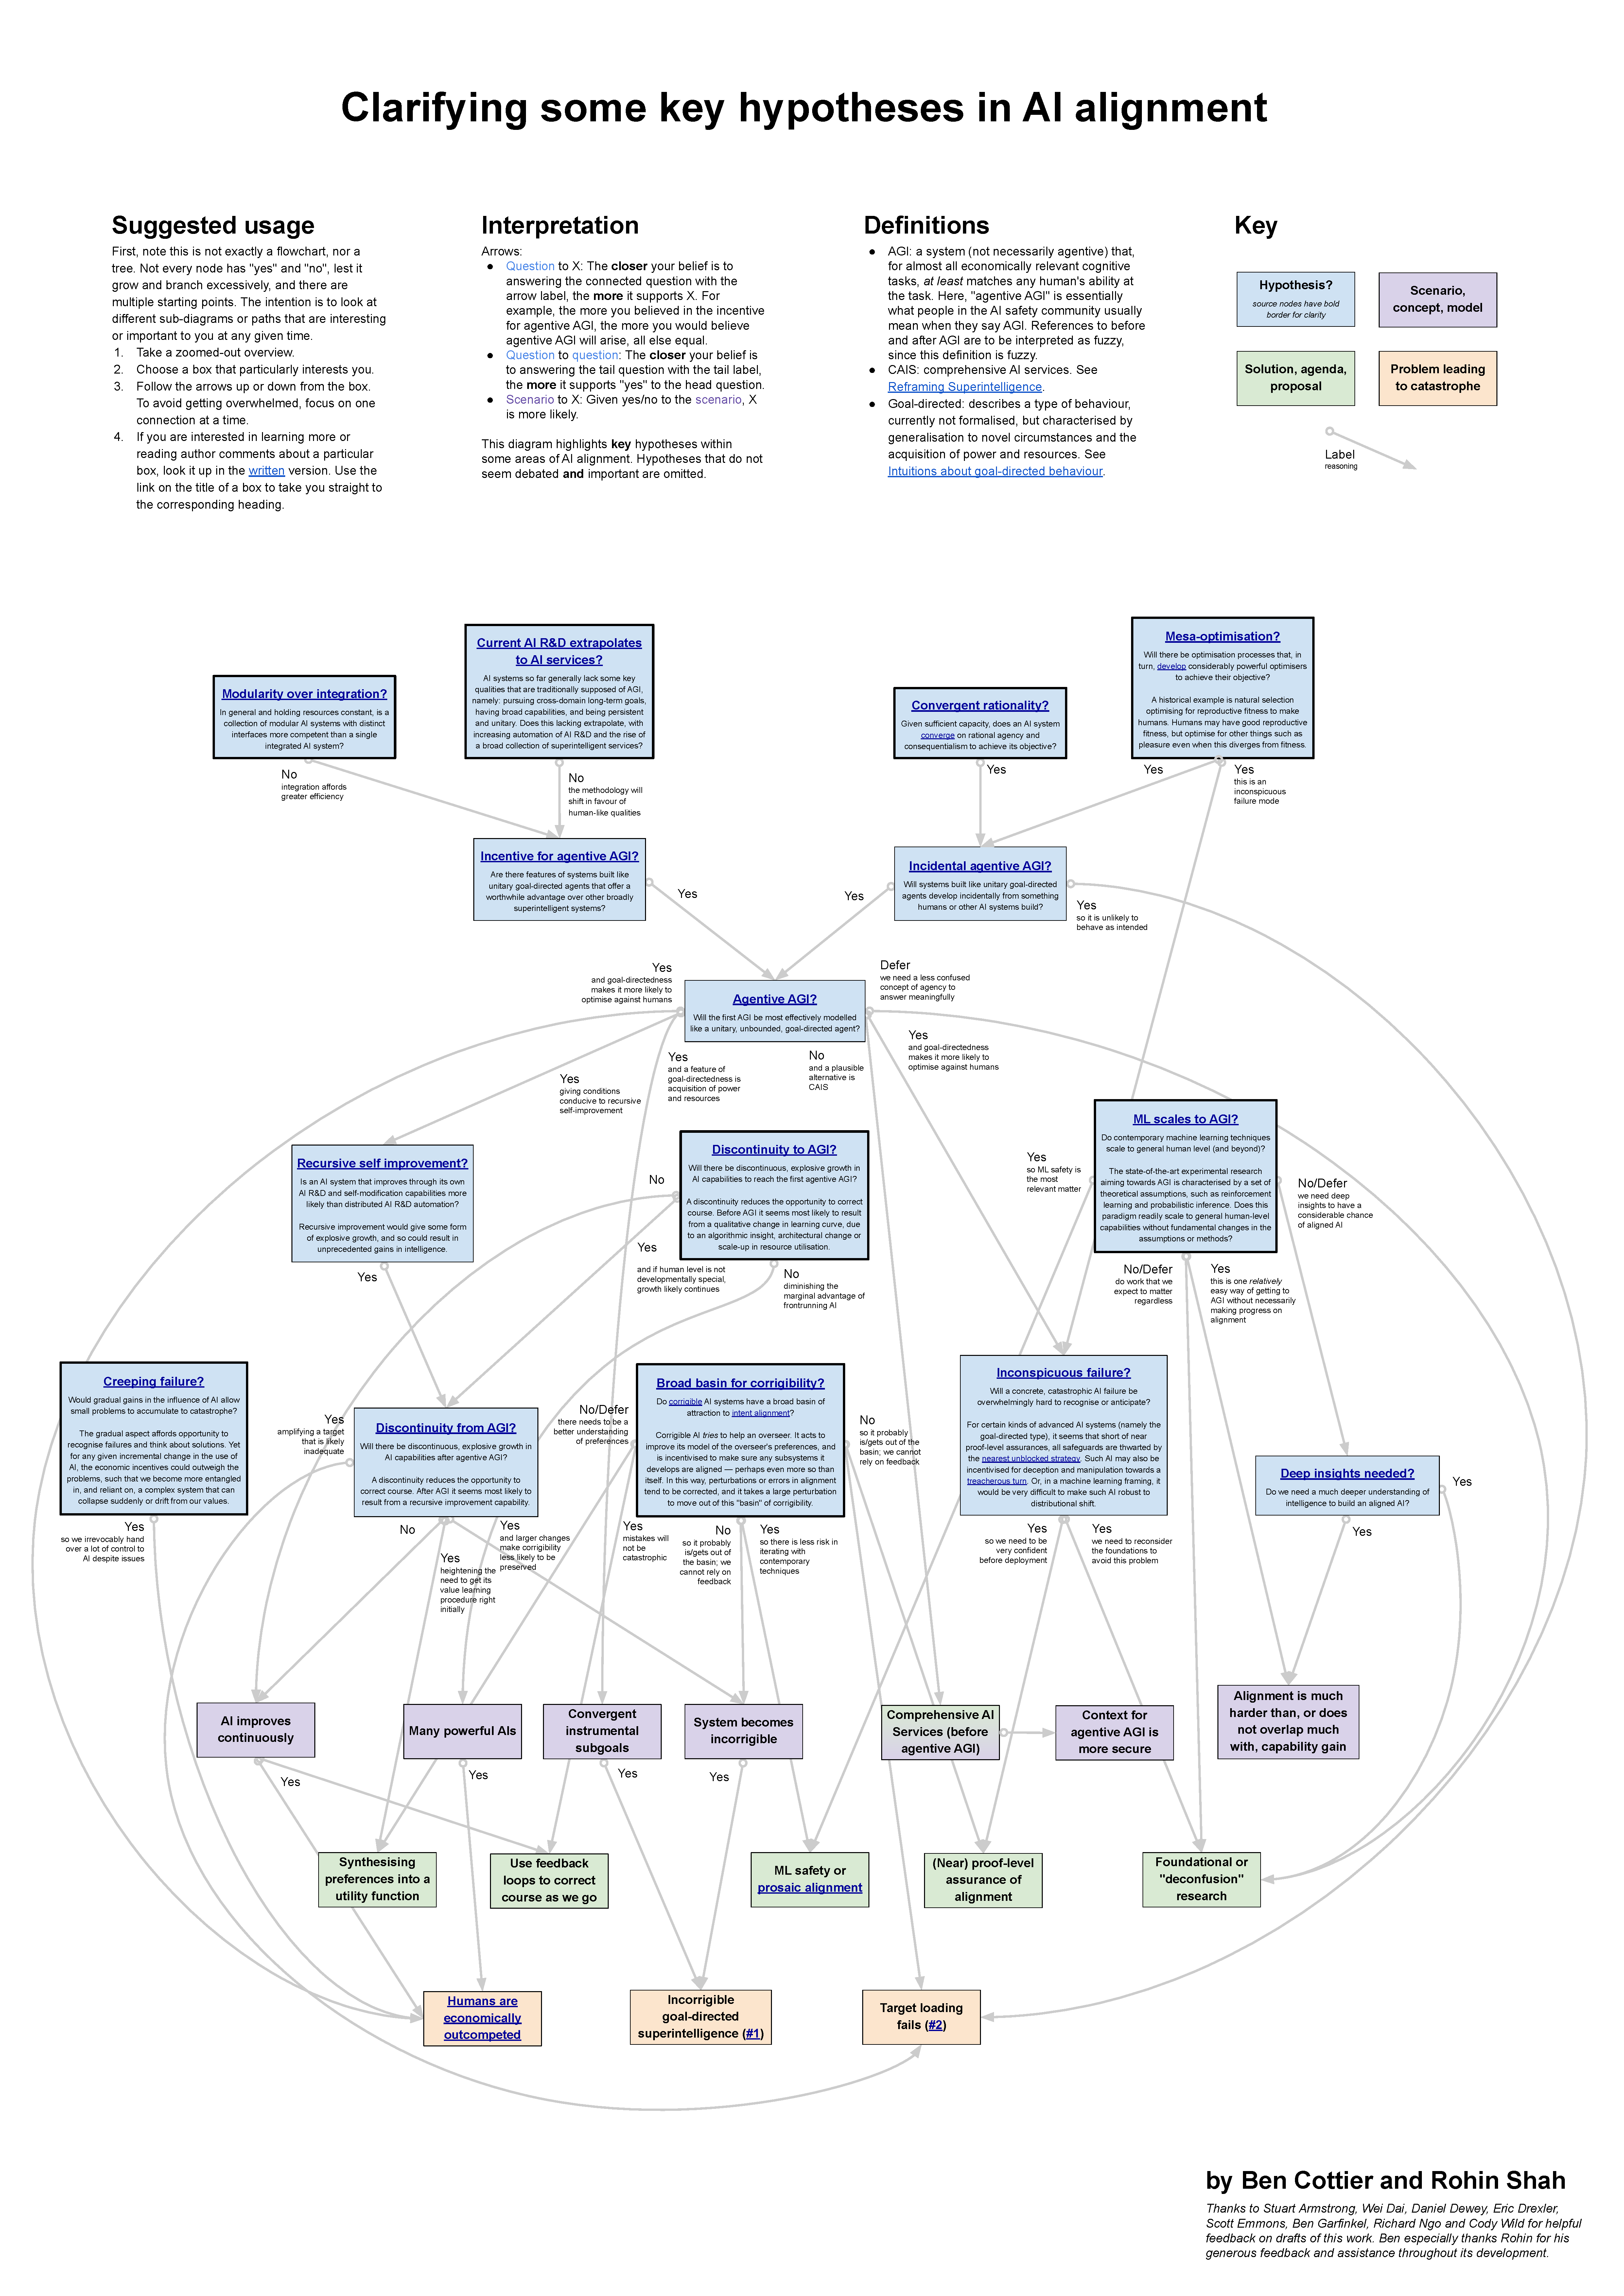
\includegraphics[width=1\linewidth,height=\textheight,keepaspectratio]{images/hypotheses_diagram.pdf}}

}

\caption[Key hypotheses in AI
alignment]{\label{fig-ai-hypotheses-map}from \textcite{cottier2019}: Key
hypotheses across the AI alignment ecosystem}

\end{figure}%

\subsection{1.2.1 Safety Gaps from Misaligned
Efforts}\label{safety-gaps-from-misaligned-efforts}

The fragmentation problem manifests in incompatible frameworks between
technical researchers, policy specialists, and strategic analysts. Each
community develops sophisticated approaches within their domain, yet
translation between domains remains primitive. This creates systematic
blind spots where risks emerge at the interfaces between technical
capabilities, institutional responses, and strategic dynamics.

When different communities operate with incompatible frameworks,
critical risks fall through the cracks. Technical researchers may solve
alignment problems under assumptions that policymakers' decisions
invalidate. Regulations optimized for current systems may inadvertently
incentivize dangerous development patterns. Without shared models of the
risk landscape, our collective efforts resemble the parable of blind men
describing an elephant---each accurate within their domain but missing
the complete picture \textcite{paul2023}.

Historical precedents demonstrate how coordination failures in
technology governance can lead to dangerous dynamics. The nuclear arms
race exemplifies how lack of coordination can create negative-sum
outcomes where all parties become less secure despite massive
investments in safety measures. Similar dynamics may emerge in AI
development without proper coordination infrastructure.

\subsection{1.2.2 Resource Misallocation}\label{resource-misallocation}

The AI safety community faces a complex tradeoff in resource allocation.
While some duplication of efforts can improve reliability through
independent verification---akin to reproducing scientific results---the
current level of fragmentation often leads to wasteful redundancy.
Multiple teams independently develop similar frameworks without building
on each other's work, creating opportunity costs where critical but
unglamorous research areas remain understaffed. Funders struggle to
identify high-impact opportunities across technical and governance
domains, lacking the epistemic infrastructure to assess where marginal
resources would have the greatest impact. This misallocation becomes
more costly as the window for establishing effective governance narrows
with accelerating AI development.

\begin{longtable}[]{@{}
  >{\raggedright\arraybackslash}p{(\linewidth - 8\tabcolsep) * \real{0.2000}}
  >{\raggedright\arraybackslash}p{(\linewidth - 8\tabcolsep) * \real{0.2000}}
  >{\raggedright\arraybackslash}p{(\linewidth - 8\tabcolsep) * \real{0.2000}}
  >{\raggedright\arraybackslash}p{(\linewidth - 8\tabcolsep) * \real{0.2000}}
  >{\raggedright\arraybackslash}p{(\linewidth - 8\tabcolsep) * \real{0.2000}}@{}}
\caption{Examples of duplicated AI safety efforts across
organizations}\label{tbl-resource-duplication}\tabularnewline
\toprule\noalign{}
\begin{minipage}[b]{\linewidth}\raggedright
Research Area
\end{minipage} & \begin{minipage}[b]{\linewidth}\raggedright
Organization A
\end{minipage} & \begin{minipage}[b]{\linewidth}\raggedright
Organization B
\end{minipage} & \begin{minipage}[b]{\linewidth}\raggedright
Duplication Level
\end{minipage} & \begin{minipage}[b]{\linewidth}\raggedright
Opportunity Cost
\end{minipage} \\
\midrule\noalign{}
\endfirsthead
\toprule\noalign{}
\begin{minipage}[b]{\linewidth}\raggedright
Research Area
\end{minipage} & \begin{minipage}[b]{\linewidth}\raggedright
Organization A
\end{minipage} & \begin{minipage}[b]{\linewidth}\raggedright
Organization B
\end{minipage} & \begin{minipage}[b]{\linewidth}\raggedright
Duplication Level
\end{minipage} & \begin{minipage}[b]{\linewidth}\raggedright
Opportunity Cost
\end{minipage} \\
\midrule\noalign{}
\endhead
\bottomrule\noalign{}
\endlastfoot
Interpretability Methods & Anthropic's mechanistic interpretability &
DeepMind's concept activation vectors & Medium & Reduced focus on
multi-agent safety \\
Alignment Frameworks & MIRI's embedded agency & FHI's comprehensive AI
services & High & Limited work on institutional design \\
Risk Assessment Models & GovAI's policy models & CSER's existential risk
frameworks & High & Insufficient capability benchmarking \\
\end{longtable}

\subsection{1.2.3 Negative-Sum Dynamics}\label{negative-sum-dynamics}

Perhaps most concerning, uncoordinated interventions can actively
increase risk. Safety standards that advantage established players may
accelerate risky development elsewhere. Partial transparency
requirements might enable capability advances without commensurate
safety improvements. International agreements lacking shared technical
understanding may lock in dangerous practices. Without coordination, our
cure risks becoming worse than the disease.

The game-theoretic structure of AI development creates particularly
pernicious dynamics. Armstrong et al. \textcite{armstrong2016}
demonstrate how uncoordinated policies can incentivize a ``race to the
precipice'' where competitive pressures override safety considerations.
The situation resembles a multi-player prisoner's dilemma or stag hunt
where individually rational decisions lead to collectively catastrophic
outcomes \textcite{samuel2023} \textcite{hunt2025}.

\section{1.3 Historical Parallels and Temporal
Urgency}\label{historical-parallels-and-temporal-urgency}

History offers instructive parallels. The nuclear age began with
scientists racing to understand and control forces that could destroy
civilization. Early coordination failures---competing national programs,
scientist-military tensions, public-expert divides---nearly led to
catastrophe multiple times. Only through developing shared frameworks
(deterrence theory) \textcite{schelling1960}, institutions (IAEA), and
communication channels (hotlines, treaties) did humanity navigate the
nuclear precipice \textcite{rehman2025}.

Yet AI presents unique coordination challenges that compress our
response timeline:

\textbf{Accelerating Development}: Unlike nuclear weapons requiring
massive infrastructure, AI development proceeds in corporate labs and
academic departments worldwide. Capability improvements come through
algorithmic insights and computational scale, both advancing
exponentially.

\textbf{Dual-Use Ubiquity}: Every AI advance potentially contributes to
both beneficial applications and catastrophic risks. The same language
model architectures enabling scientific breakthroughs could facilitate
dangerous manipulation or deception at scale.

\textbf{Comprehension Barriers}: Nuclear risks were viscerally
understandable---cities vaporized, radiation sickness, nuclear winter.
AI risks involve abstract concepts like optimization processes, goal
misspecification, and emergent capabilities that resist intuitive
understanding.

\textbf{Governance Lag}: Traditional governance
mechanisms---legislation, international treaties, professional
standards---operate on timescales of years to decades. AI capabilities
advance on timescales of months to years, creating an ever-widening
capability-governance gap.

\section{1.4 Research Question and
Scope}\label{research-question-and-scope}

This thesis addresses a specific dimension of the coordination challenge
by investigating the question:

\textbf{Can frontier AI technologies be utilized to automate the
modeling of transformative AI risks, enabling robust prediction of
policy impacts across diverse worldviews?}

More specifically, I explore whether frontier language models can
automate the extraction and formalization of probabilistic world models
from AI safety literature, creating a scalable computational framework
that enhances coordination in AI governance through systematic policy
evaluation under uncertainty.

To break this down into its components:

\begin{itemize}
\tightlist
\item
  \textbf{Frontier AI Technologies}: Today's most capable language
  models (GPT-4, Claude-3 level systems)
\item
  \textbf{Automated Modeling}: Using these systems to extract and
  formalize argument structures from natural language
\item
  \textbf{Transformative AI Risks}: Potentially catastrophic outcomes
  from advanced AI systems, particularly existential risks
\item
  \textbf{Policy Impact Prediction}: Evaluating how governance
  interventions might alter probability distributions over outcomes
\item
  \textbf{Diverse Worldviews}: Accounting for fundamental disagreements
  about AI development trajectories and risk factors
\end{itemize}

The investigation encompasses both theoretical development and practical
implementation, focusing specifically on existential risks from
misaligned AI systems rather than broader AI ethics concerns. This
narrowed scope enables deep technical development while addressing the
highest-stakes coordination challenges.

\section{1.5 The Multiplicative Benefits
Framework}\label{the-multiplicative-benefits-framework}

The central thesis of this work is that combining three
elements---automated worldview extraction, prediction market
integration, and formal policy evaluation---creates multiplicative
rather than merely additive benefits for AI governance. Each component
enhances the others, creating a system more valuable than the sum of its
parts.

\subsection{1.5.1 Automated Worldview
Extraction}\label{automated-worldview-extraction}

Current approaches to AI risk modeling, exemplified by the Modeling
Transformative AI Risks (MTAIR) project, demonstrate the value of formal
representation but require extensive manual effort. Creating a single
model demands dozens of expert-hours to translate qualitative arguments
into quantitative frameworks. This bottleneck severely limits the number
of perspectives that can be formalized and the speed of model updates as
new arguments emerge.

Automation using frontier language models addresses this scaling
challenge. By developing systematic methods to extract causal structures
and probability judgments from natural language, we can:

\begin{itemize}
\tightlist
\item
  Process orders of magnitude more content
\item
  Incorporate diverse perspectives rapidly
\item
  Maintain models that evolve with the discourse
\item
  Reduce barriers to entry for contributing worldviews
\end{itemize}

\subsection{1.5.2 Live Data Integration}\label{live-data-integration}

Static models, however well-constructed, quickly become outdated in
fast-moving domains. Prediction markets and forecasting platforms
aggregate distributed knowledge about uncertain futures, providing
continuously updated probability estimates. By connecting formal models
to these live data sources, we create dynamic assessments that
incorporate the latest collective intelligence \textcite{tetlock2015}.

This integration serves multiple purposes:

\begin{itemize}
\tightlist
\item
  Grounding abstract models in empirical forecasts
\item
  Identifying which uncertainties most affect outcomes
\item
  Revealing when model assumptions diverge from collective expectations
\item
  Generating new questions for forecasting communities
\end{itemize}

\subsection{1.5.3 Formal Policy
Evaluation}\label{formal-policy-evaluation}

\textbf{Formal policy evaluation} transforms static risk assessments
into actionable guidance by modeling how specific interventions alter
critical parameters. Using causal inference techniques
\textcite{pearl2000} \textcite{pearl2009}, we can assess not just the
probability of adverse outcomes but how those probabilities change under
different policy regimes.

This enables genuinely evidence-based policy development:

\begin{itemize}
\tightlist
\item
  Comparing interventions across multiple worldviews
\item
  Identifying robust strategies that work across scenarios
\item
  Understanding which uncertainties most affect policy effectiveness
\item
  Prioritizing research to reduce decision-relevant uncertainty
\end{itemize}

\subsection{1.5.4 The Synergy}\label{the-synergy}

The multiplicative benefits emerge from the interactions between
components:

\begin{itemize}
\tightlist
\item
  Automation enables comprehensive coverage, making prediction market
  integration more valuable by connecting to more perspectives
\item
  Market data validates and calibrates automated extractions, improving
  quality
\item
  Policy evaluation gains precision from both comprehensive models and
  live probability updates
\item
  The complete system creates feedback loops where policy analysis
  identifies critical uncertainties for market attention
\end{itemize}

This synergistic combination addresses the coordination crisis by
providing common ground for disparate communities, translating between
technical and policy languages, quantifying previously implicit
disagreements, and enabling evidence-based compromise.

\section{1.6 Thesis Structure and
Roadmap}\label{thesis-structure-and-roadmap}

The remainder of this thesis develops the multiplicative benefits
framework from theoretical foundations to practical implementation:

\textbf{Chapter 2: Context and Theoretical Foundations} establishes the
intellectual groundwork, examining the epistemic challenges unique to AI
governance, Bayesian networks as formal tools for uncertainty
representation, argument mapping as a bridge from natural language to
formal models, the MTAIR project's achievements and limitations, and
requirements for effective coordination infrastructure.

\textbf{Chapter 3: AMTAIR Design and Implementation} presents the
technical system including overall architecture and design principles,
the two-stage extraction pipeline (ArgDown → BayesDown), validation
methodology and results, case studies from simple examples to complex AI
risk models, and integration with prediction markets and policy
evaluation.

\textbf{Chapter 4: Discussion - Implications and Limitations} critically
examines technical limitations and failure modes, conceptual concerns
about formalization, integration with existing governance frameworks,
scaling challenges and opportunities, and broader implications for
epistemic security.

\textbf{Chapter 5: Conclusion} synthesizes key contributions and charts
paths forward with a summary of theoretical and practical achievements,
concrete recommendations for stakeholders, research agenda for community
development, and vision for AI governance with proper coordination
infrastructure.

Throughout this progression, I maintain dual focus on theoretical
sophistication and practical utility. The framework aims not merely to
advance academic understanding but to provide actionable tools for
improving coordination in AI governance during this critical period.

Having established the coordination crisis and outlined how automated
modeling can address it, we now turn to the theoretical foundations that
make this approach possible. The next chapter examines the unique
epistemic challenges of AI governance and introduces the formal
tools---particularly Bayesian networks---that enable rigorous reasoning
under deep uncertainty.

\bookmarksetup{startatroot}

\chapter{2. Context and Theoretical
Foundations}\label{context-and-theoretical-foundations}

This chapter establishes the theoretical and methodological foundations
for the AMTAIR approach. We begin by examining a concrete example of
structured AI risk assessment---Joseph Carlsmith's power-seeking AI
model---to ground our discussion in practical terms. We then explore the
unique epistemic challenges of AI governance that render traditional
policy analysis inadequate, introduce Bayesian networks as formal tools
for representing uncertainty, and examine how argument mapping bridges
natural language reasoning and formal models. The chapter concludes by
analyzing the MTAIR project's achievements and limitations, motivating
the need for automated approaches, and surveying relevant literature
across AI risk modeling, governance proposals, and technical
methodologies.

\section{2.1 AI Existential Risk: The Carlsmith
Model}\label{ai-existential-risk-the-carlsmith-model}

To ground our discussion in concrete terms, I examine Joseph Carlsmith's
``Is Power-Seeking AI an Existential Risk?'' as an exemplar of
structured reasoning about AI catastrophic risk
\textcite{carlsmith2022}. Carlsmith's analysis stands out for its
explicit probabilistic decomposition of the path from current AI
development to potential existential catastrophe.

\subsection{2.1.1 Six-Premise
Decomposition}\label{six-premise-decomposition}

According to the MTAIR model \textcite{clarke2022}, Carlsmith decomposes
existential risk into a probabilistic chain with explicit
estimates\footnote{Multiple versions of Carlsmith's paper exist with
  slight updates to probability estimates: \textcite{carlsmith2021},
  \textcite{carlsmith2022}, \textcite{carlsmith2024}. We primarily
  reference the version used by the MTAIR team for their extraction.
  Extended discussion and expert probability estimates can be found on
  LessWrong.}:

\begin{enumerate}
\def\labelenumi{\arabic{enumi}.}
\tightlist
\item
  \textbf{Premise}: Transformative AI development this
  century\footnote{\textbf{Premise 1: APS Systems by 2070} \((P≈0.65)\)
    ``By 2070, there will be AI systems with Advanced capability,
    Agentic planning, and Strategic awareness''---the conjunction of
    capabilities that could enable systematic pursuit of objectives in
    the world.} \((P≈0.80)\)\footnote{\textbf{Premise 1: APS Systems by
    2070} \((P≈0.65)\) ``By 2070, there will be AI systems with Advanced
    capability, Agentic planning, and Strategic awareness''---the
    conjunction of capabilities that could enable systematic pursuit of
    objectives in the world.}
\item
  \textbf{Premise}: AI systems pursuing objectives in the
  world\footnote{\textbf{Premise 2: Alignment Difficulty} \((P≈0.40)\)
    ``It will be harder to build aligned APS systems than misaligned
    systems that are still attractive to deploy''---capturing the
    challenge that safety may conflict with capability or efficiency.}
  \((P≈0.95)\)
\item
  \textbf{Premise}: Systems with power-seeking instrumental
  incentives\footnote{\textbf{Premise 3: Deployment Despite
    Misalignment} \((P≈0.70)\) ``Conditional on 1 and 2, we will deploy
    misaligned APS systems''---reflecting competitive pressures and
    limited coordination.} \((P≈0.40)\)
\item
  \textbf{Premise}: Sufficient capability for existential
  threat\footnote{\textbf{Premise 4: Power-Seeking Behavior}
    \((P≈0.65)\) ``Conditional on 1-3, misaligned APS systems will seek
    power in high-impact ways''---based on instrumental convergence
    arguments.} \((P≈0.65)\)
\item
  \textbf{Premise}: Misaligned systems despite safety efforts\footnote{\textbf{Premise
    5: Disempowerment Success} \((P≈0.40)\) ``Conditional on 1-4,
    power-seeking will scale to permanent human
    disempowerment''---despite potential resistance and safeguards.}
  \((P≈0.50)\)
\item
  \textbf{Premise}: Catastrophic outcomes from misaligned
  power-seeking\footnote{\textbf{Premise 6: Existential Catastrophe}
    \((P≈0.95)\) ``Conditional on 1-5, this disempowerment constitutes
    existential catastrophe''---connecting power loss to permanent
    curtailment of human potential.} \((P≈0.65)\)
\end{enumerate}

\textbf{Composite Risk Calculation}\footnote{\textbf{Overall Risk}:
  Multiplying through the conditional chain yields \$P(doom)≈0.05 \$ or
  5\% by 2070.}: \(P(doom)≈0.05\) (5\%)

This structured approach exemplifies the type of reasoning AMTAIR aims
to formalize and automate. While Carlsmith spent months developing this
model manually, similar rigor exists implicitly in many AI safety
arguments awaiting extraction.

\begin{figure}

\centering{

\href{https://www.lesswrong.com/posts/sGkRDrpphsu6Jhega/a-model-based-approach-to-ai-existential-risk}{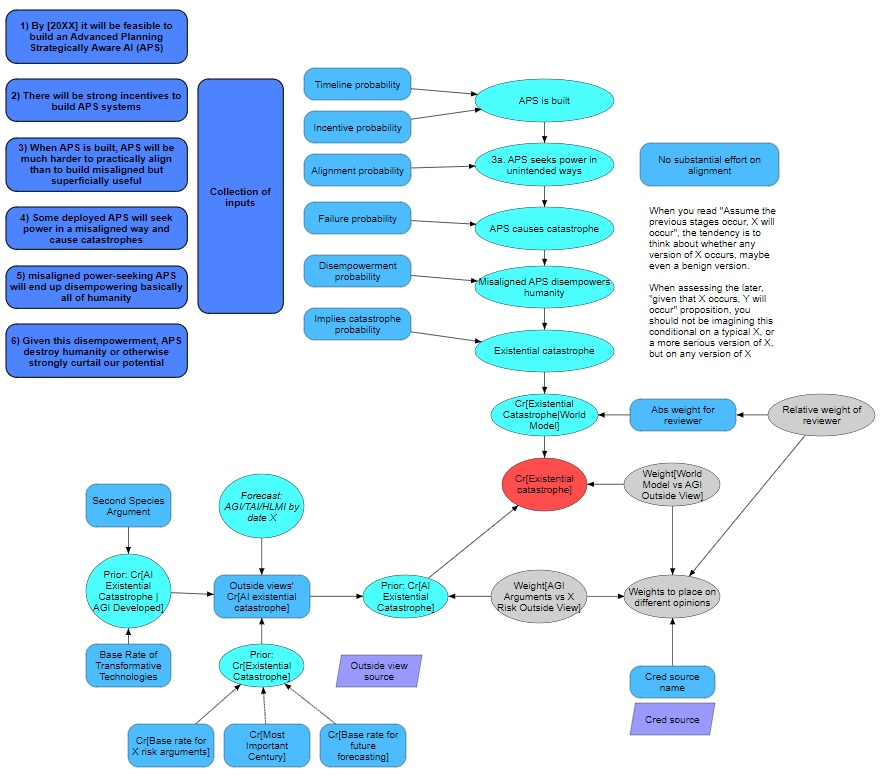
\includegraphics[width=1.2\linewidth,height=\textheight,keepaspectratio]{images/mtair-insideoutside-base.jpg}}

}

\caption[Base APS causal map
(clean)]{\label{fig-mtair-insideoutside-base}from
\textcite{manheim2021}: MTAIR integrated Carlsmith's model as the
``inside view'' in their Analytica Software Demonstration}

\end{figure}%

\subsection{2.1.2 Why Carlsmith Exemplifies Formalizable
Arguments}\label{why-carlsmith-exemplifies-formalizable-arguments}

Carlsmith's model demonstrates several features that make it ideal for
formal representation:

\textbf{Explicit Probabilistic Structure}: Each premise receives
numerical probability estimates with documented reasoning, enabling
direct translation to Bayesian network parameters.

\textbf{Clear Conditional Dependencies}: The logical flow from
capabilities through deployment decisions to catastrophic outcomes maps
naturally onto directed acyclic graphs.

\textbf{Transparent Decomposition}: Breaking the argument into modular
premises allows independent evaluation and sensitivity analysis of each
component.

\textbf{Documented Reasoning}: Extensive justification for each
probability enables extraction of both structure and parameters from the
source text.

We will return to Carlsmith's model in Chapter 3 as our primary complex
case study, demonstrating how AMTAIR successfully extracts and
formalizes this sophisticated multi-level argument.

Beyond Carlsmith's model, other structured approaches to AI risk---such
as Christiano's ``What failure looks like''
\textcite{christiano2019}---provide additional targets for automated
extraction, enabling comparative analysis across different expert
worldviews.

\section{2.2 The Epistemic Challenge of Policy
Evaluation}\label{the-epistemic-challenge-of-policy-evaluation}

AI governance policy evaluation faces unique epistemic challenges that
render traditional policy analysis methods insufficient. Understanding
these challenges motivates the need for new computational approaches.

\subsection{2.2.1 Unique Characteristics of AI
Governance}\label{unique-characteristics-of-ai-governance}

\textbf{Deep Uncertainty Rather Than Risk}: Traditional policy analysis
distinguishes between risk (known probability distributions) and
uncertainty (known possibilities, unknown probabilities). AI governance
faces deep uncertainty---we cannot confidently enumerate possible
futures, much less assign probabilities \textcite{hallegatte2012}. Will
recursive self-improvement enable rapid capability gains? Can value
alignment be solved technically? These foundational questions resist
empirical resolution before their answers become catastrophically
relevant.

\textbf{Complex Multi-Level Causation}: Policy effects propagate through
technical, institutional, and social levels with intricate feedback
loops. A technical standard might alter research incentives, shifting
capability development trajectories, changing competitive dynamics, and
ultimately affecting existential risk through pathways invisible at the
policy's inception. Traditional linear causal models cannot capture
these dynamics.

\textbf{Irreversibility and Lock-In}: Many AI governance decisions
create path dependencies that prove difficult or impossible to reverse.
Early technical standards shape development trajectories. Institutional
structures ossify. International agreements create sticky equilibria.
Unlike many policy domains where course correction remains possible, AI
governance mistakes may prove permanent.

\textbf{Value-Laden Technical Choices}: The entanglement of technical
and normative questions confounds traditional separation of facts and
values. What constitutes ``alignment''? How much capability development
should we risk for economic benefits? Technical specifications embed
ethical judgments that resist neutral expertise.

\begin{longtable}[]{@{}
  >{\raggedright\arraybackslash}p{(\linewidth - 4\tabcolsep) * \real{0.3333}}
  >{\raggedright\arraybackslash}p{(\linewidth - 4\tabcolsep) * \real{0.3333}}
  >{\raggedright\arraybackslash}p{(\linewidth - 4\tabcolsep) * \real{0.3333}}@{}}
\caption{Comparison of AI governance vs traditional policy
domains}\label{tbl-governance-challenges}\tabularnewline
\toprule\noalign{}
\begin{minipage}[b]{\linewidth}\raggedright
Dimension
\end{minipage} & \begin{minipage}[b]{\linewidth}\raggedright
Traditional Policy
\end{minipage} & \begin{minipage}[b]{\linewidth}\raggedright
AI Governance
\end{minipage} \\
\midrule\noalign{}
\endfirsthead
\toprule\noalign{}
\begin{minipage}[b]{\linewidth}\raggedright
Dimension
\end{minipage} & \begin{minipage}[b]{\linewidth}\raggedright
Traditional Policy
\end{minipage} & \begin{minipage}[b]{\linewidth}\raggedright
AI Governance
\end{minipage} \\
\midrule\noalign{}
\endhead
\bottomrule\noalign{}
\endlastfoot
Uncertainty Type & Risk (known distributions) & Deep uncertainty
(unknown unknowns) \\
Causal Structure & Linear, traceable & Multi-level, feedback loops \\
Reversibility & Course correction possible & Path dependencies,
lock-in \\
Fact-Value Separation & Clear boundaries & Entangled
technical-normative \\
Empirical Grounding & Historical precedents & Unprecedented phenomena \\
Time Horizons & Years to decades & Months to centuries \\
\end{longtable}

\subsection{2.2.2 Limitations of Traditional
Approaches}\label{limitations-of-traditional-approaches}

Standard policy evaluation tools prove inadequate for these challenges:

\textbf{Cost-Benefit Analysis} assumes commensurable outcomes and stable
probability distributions. When potential outcomes include existential
catastrophe with deeply uncertain probabilities, the mathematical
machinery breaks down. Infinite negative utility resists standard
decision frameworks.

\textbf{Scenario Planning} helps explore possible futures but typically
lacks the probabilistic reasoning needed for decision-making under
uncertainty. Without quantification, scenarios provide narrative
richness but limited action guidance.

\textbf{Expert Elicitation} aggregates specialist judgment but struggles
with interdisciplinary questions where no single expert grasps all
relevant factors. Moreover, experts often operate with different
implicit models, making aggregation problematic.

\textbf{Red Team Exercises} test specific plans but miss systemic risks
emerging from component interactions. Gaming individual failures cannot
reveal emergent catastrophic possibilities.

These limitations create a methodological gap: we need approaches that
handle deep uncertainty, represent complex causation, quantify expert
disagreement, and enable systematic exploration of intervention effects.

\subsection{2.2.3 The Underlying Epistemic
Framework}\label{the-underlying-epistemic-framework}

The AMTAIR approach rests on a specific epistemic framework that
combines probabilistic reasoning, conditional logic, and possible worlds
semantics. This framework provides the philosophical foundation for
representing deep uncertainty about AI futures.

\textbf{Probabilistic Epistemology}: Following the Bayesian tradition,
we treat probability as a measure of rational credence rather than
objective frequency. This subjective interpretation allows meaningful
probability assignments even for unique, unprecedented events like AI
catastrophe. As E.T. Jaynes demonstrated, probability theory extends
deductive logic to handle uncertainty, providing a calculus for rational
belief \textcite{jaynes2003}.

\textbf{Conditional Structure}: The framework emphasizes conditional
rather than absolute probabilities. Instead of asking ``What is
P(catastrophe)?'' we ask ``What is P(catastrophe \textbar{} specific
assumptions)?'' This conditionalization makes explicit the dependency of
conclusions on worldview assumptions, enabling productive disagreement
about premises rather than conclusions.

\textbf{Possible Worlds Semantics}: We conceptualize uncertainty as
distributions over possible worlds---complete descriptions of how
reality might unfold. Each world represents a coherent scenario with
specific values for all relevant variables. Probability distributions
over these worlds capture both what we know and what we don't know about
the future.

This framework enables several key capabilities:

\begin{enumerate}
\def\labelenumi{\arabic{enumi}.}
\tightlist
\item
  \textbf{Representing ignorance}: We can express uncertainty about
  uncertainty itself through hierarchical probability models
\item
  \textbf{Combining evidence}: Bayesian updating provides principled
  methods for integrating new information
\item
  \textbf{Comparing worldviews}: Different probability distributions
  over the same space of possibilities enable systematic comparison
\item
  \textbf{Evaluating interventions}: Counterfactual reasoning about how
  actions change probability distributions
\end{enumerate}

\subsection{2.2.4 Toward New Epistemic
Tools}\label{toward-new-epistemic-tools}

The inadequacy of traditional methods for AI governance creates an
urgent need for new epistemic tools. These tools must:

\begin{itemize}
\tightlist
\item
  \textbf{Handle Deep Uncertainty}: Move beyond point estimates to
  represent ranges of possibilities
\item
  \textbf{Capture Complex Causation}: Model multi-level interactions and
  feedback loops
\item
  \textbf{Quantify Disagreement}: Make explicit where experts diverge
  and why
\item
  \textbf{Enable Systematic Analysis}: Support rigorous comparison of
  policy options
\end{itemize}

\textbf{Key Insight}: The computational approaches developed in this
thesis---particularly Bayesian networks enhanced with automated
extraction---directly address each of these requirements by providing
formal frameworks for reasoning under uncertainty.

\begin{figure}

\centering{

\href{https://static1.squarespace.com/static/635693acf15a3e2a14a56a4a/t/66ba37a144f1d6095de467df/1723479995772/AIConditionalTrees.pdf\#page=5.78}{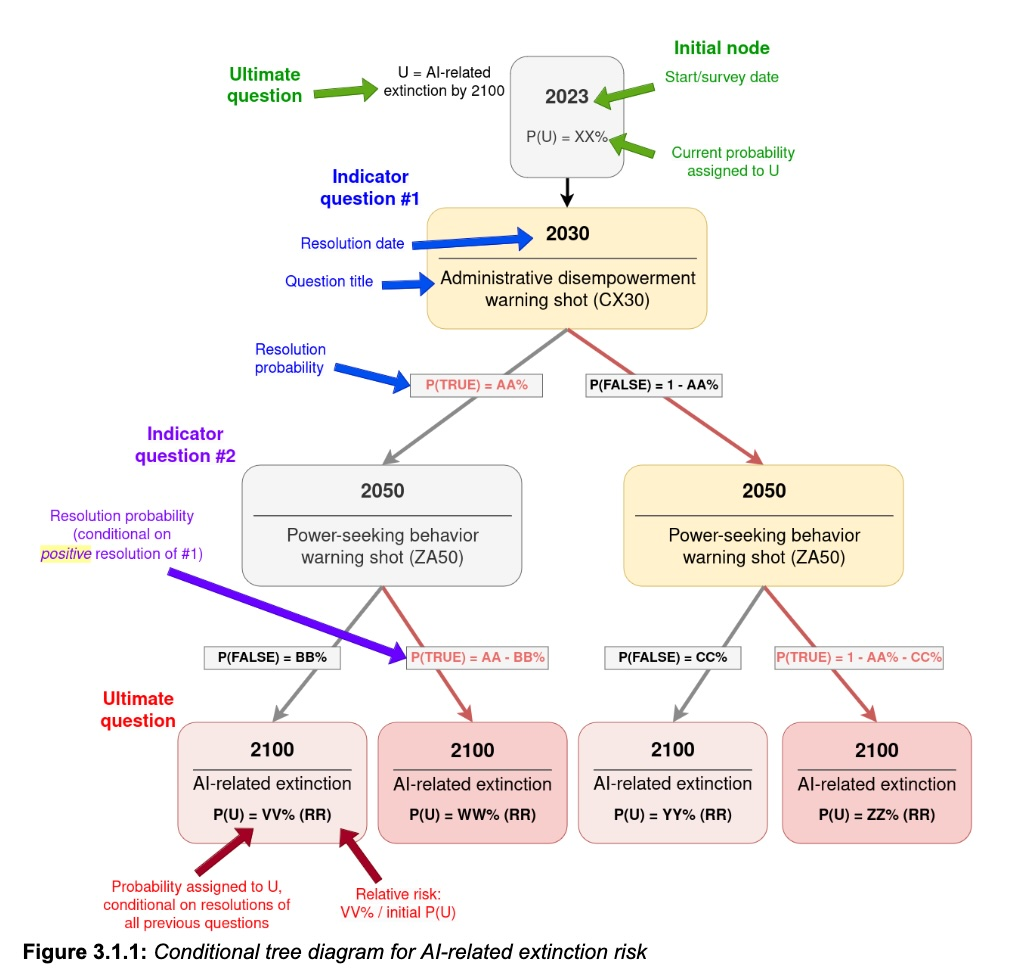
\includegraphics[width=0.8\linewidth,height=\textheight,keepaspectratio]{images/conditional_tree.jpg}}

}

\caption[Conditional-tree Guide]{\label{fig-conditional_tree}from
\textcite{mccaslin2024}: Conditional-tree Guide}

\end{figure}%

\begin{figure}

\centering{

\href{https://static1.squarespace.com/static/635693acf15a3e2a14a56a4a/t/66ba37a144f1d6095de467df/1723479995772/AIConditionalTrees.pdf\#page=5.78}{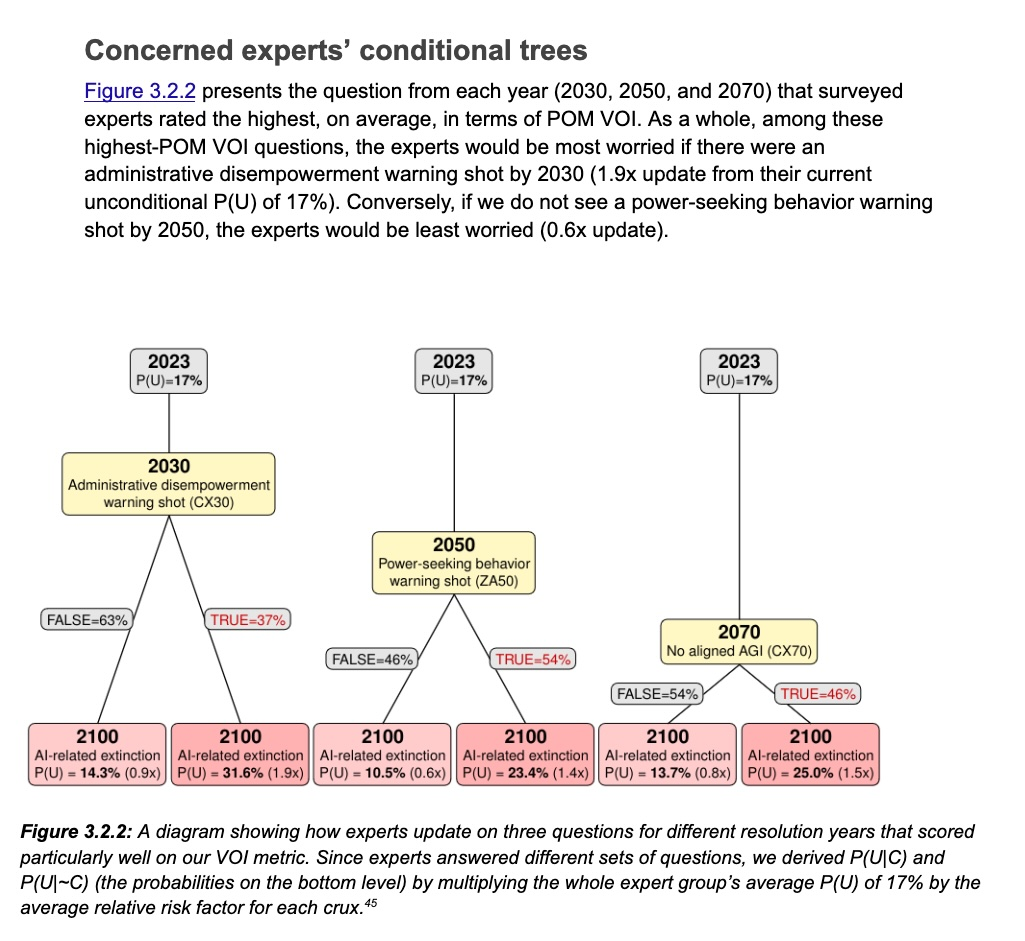
\includegraphics[width=0.8\linewidth,height=\textheight,keepaspectratio]{images/concerned_experts.jpg}}

}

\caption[Experts' conditional-tree updates
(2030-2070)]{\label{fig-concerned_experts}from \textcite{mccaslin2024}:
Experts' conditional-tree updates (2030-2070)}

\end{figure}%

Recent work on conditional trees demonstrates the value of structured
approaches to uncertainty. McCaslin et al. \textcite{mccaslin2024} show
how hierarchical conditional forecasting can identify high-value
questions for reducing uncertainty about complex topics like AI risk.
Their methodology, which asks experts to produce simplified Bayesian
networks of informative forecasting questions, achieved nine times
higher information value than standard forecasting platform questions.

Tetlock's work with the Forecasting Research Institute
\textcite{tetlock2022} exemplifies how prediction markets can provide
empirical grounding for formal models. By structuring questions as
conditional trees, they enable forecasters to express complex
dependencies between events, providing exactly the type of data needed
for Bayesian network parameterization.

\begin{figure}

\centering{

\href{https://www.metaculus.com/tournament/3508/}{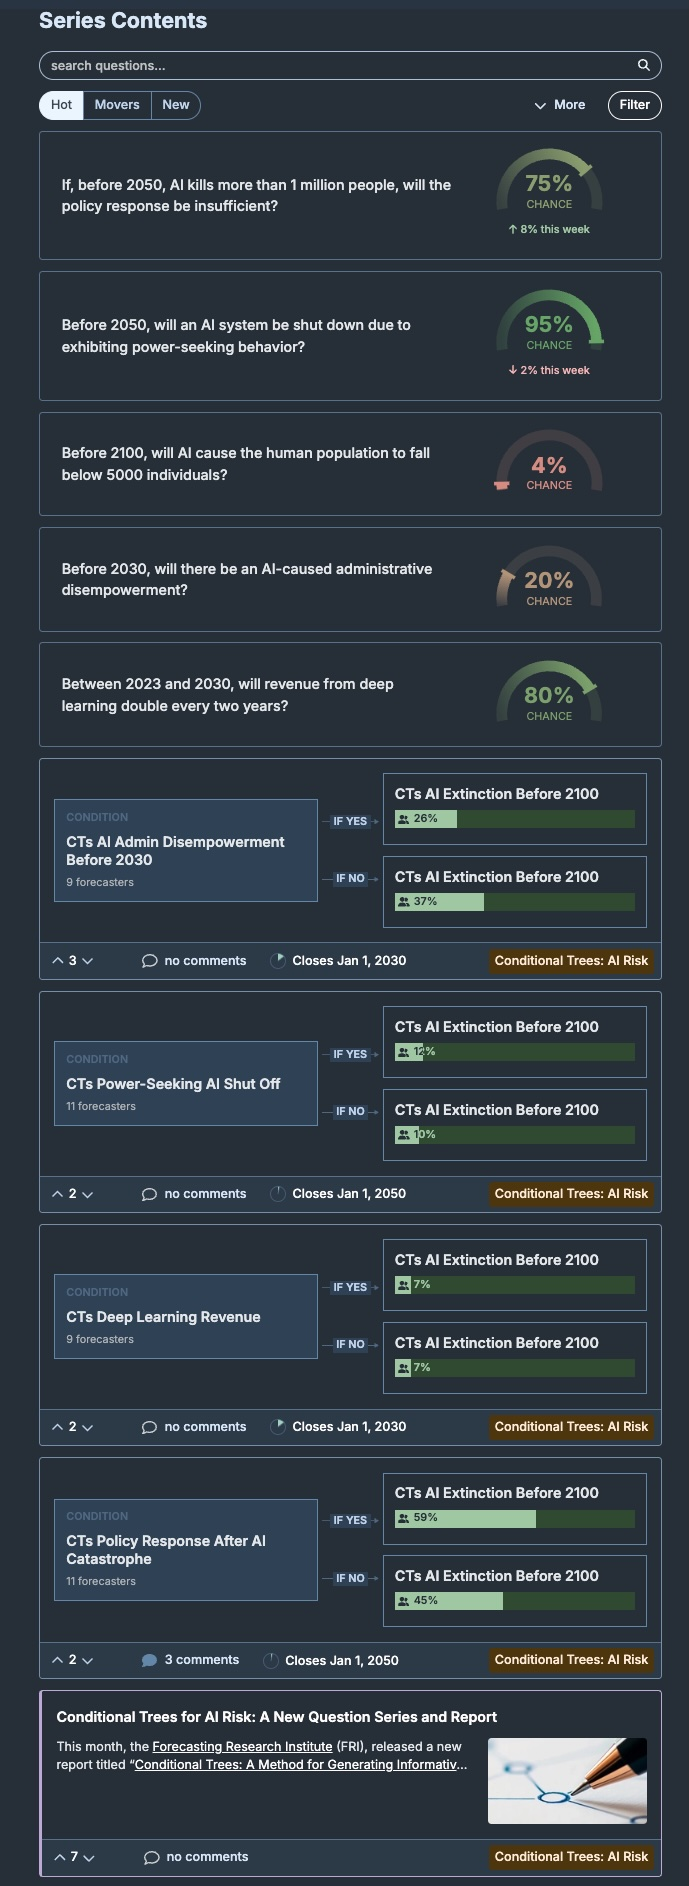
\includegraphics[width=0.8\linewidth,height=\textheight,keepaspectratio]{images/conditional_metaculus.jpg}}

}

\caption[Conditional-tree AI-risk
forecasts]{\label{fig-conditional_metaculus}from \textcite{tetlock2022}:
Conditional-tree AI-risk forecasts}

\end{figure}%

Gruetzemacher \textcite{gruetzemacher2022} evaluates the tradeoffs
between full Bayesian networks and conditional trees for forecasting
tournaments. While conditional trees offer simplicity, Bayesian networks
provide richer representation of dependencies---motivating AMTAIR's
approach of using full networks while leveraging conditional tree
insights for question generation.

\begin{figure}

\centering{

\href{https://bnma.co/uai2022-apps-workshop/papers/S5.pdf}{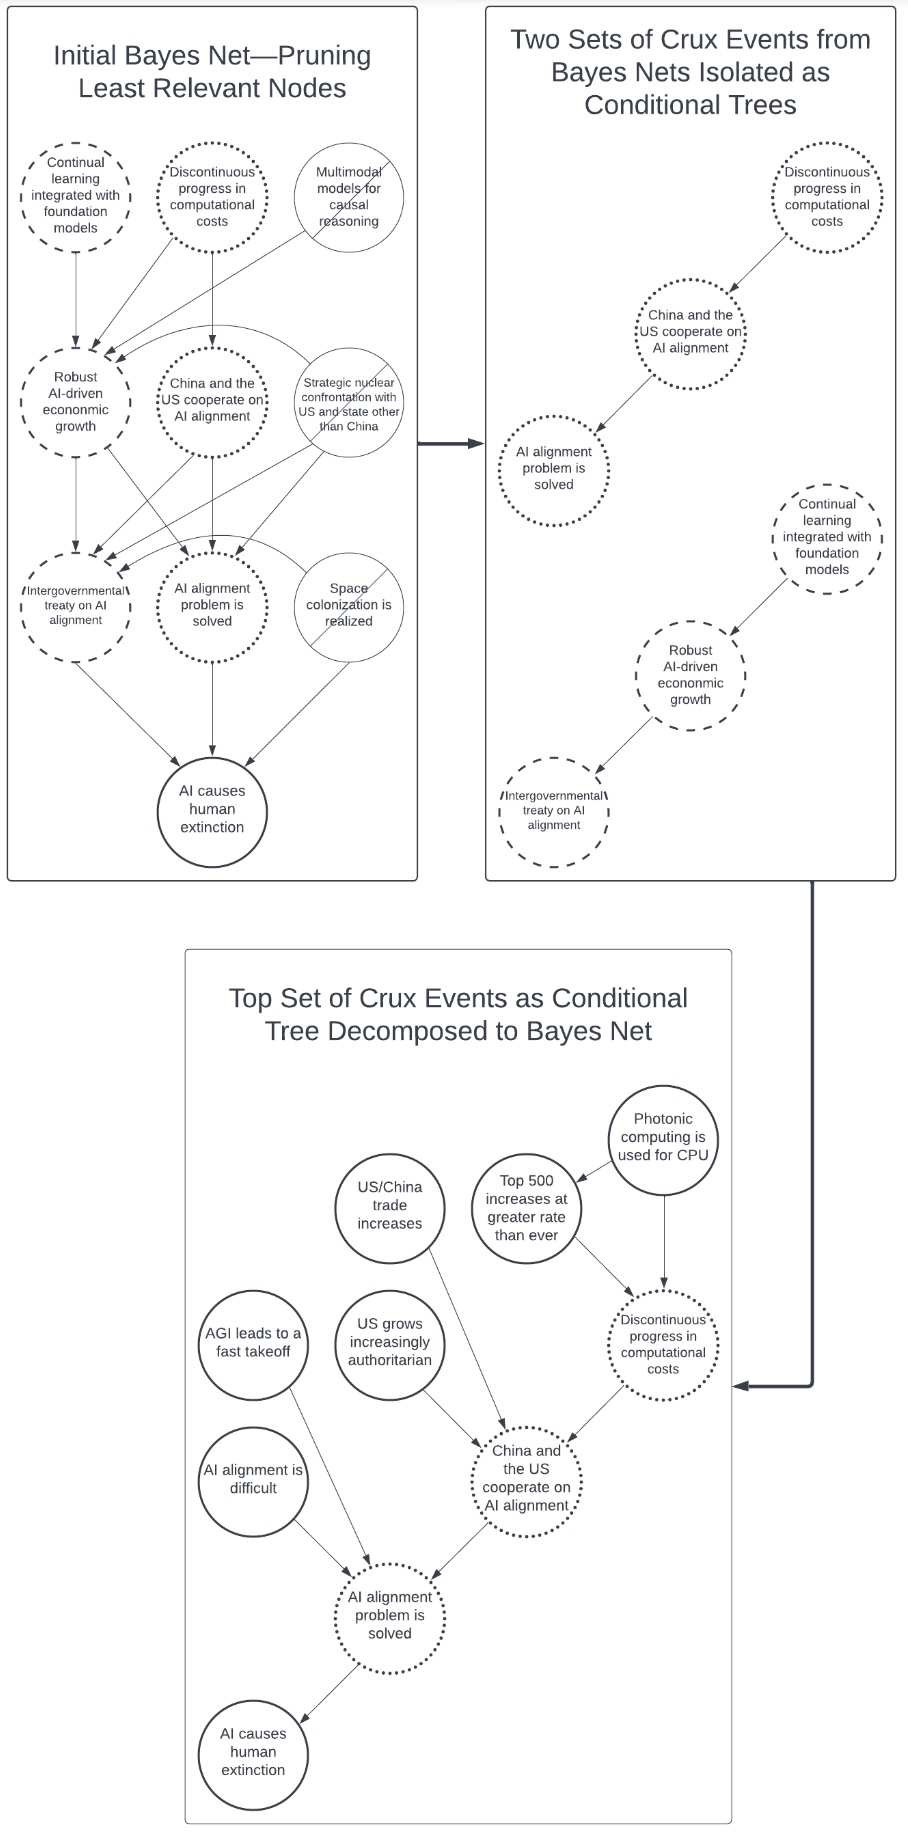
\includegraphics[width=1\linewidth,height=\textheight,keepaspectratio]{images/bns_and_conditional_trees.jpg}}

}

\caption[Bayes-net pruning → crux extraction →
re-expansion]{\label{fig-bayesnet-crux-flow}from
\textcite{gruetzemacher2022}: Bayes-net pruning → crux extraction →
re-expansion}

\end{figure}%

\section{2.3 Bayesian Networks as Knowledge
Representation}\label{bayesian-networks-as-knowledge-representation}

Bayesian networks offer a mathematical framework uniquely suited to
addressing these epistemic challenges. By combining graphical structure
with probability theory, they provide tools for reasoning about complex
uncertain domains.

\subsection{2.3.1 Mathematical
Foundations}\label{mathematical-foundations}

A Bayesian network consists of:

\begin{itemize}
\tightlist
\item
  \textbf{Directed Acyclic Graph (DAG)}: Nodes represent variables,
  edges represent direct dependencies
\item
  \textbf{Conditional Probability Tables (CPTs)}: For each node,
  P(node\textbar parents) quantifies relationships
\end{itemize}

The joint probability distribution factors according to the graph
structure:

P(X1,X2,\ldots,Xn)=∏i=1nP(Xi∣Parents(Xi))P(X\_1, X\_2, \ldots, X\_n) =
\prod\_\{i=1\}\^{}\{n\} P(X\_i \textbar{}
Parents(X\_i))P(X1\hspace{0pt},X2\hspace{0pt},\ldots,Xn\hspace{0pt})=i=1∏n\hspace{0pt}P(Xi\hspace{0pt}∣Parents(Xi\hspace{0pt}))

This factorization enables efficient inference and embodies causal
assumptions explicitly.

Pearl's foundational work \textcite{pearl2014} established Bayesian
networks as a principled approach to automated reasoning under
uncertainty, providing both theoretical foundations and practical
algorithms.

\subsection{2.3.2 The Rain-Sprinkler-Grass
Example}\label{the-rain-sprinkler-grass-example}

The canonical example illustrates key concepts\footnote{This example,
  while simple, demonstrates all essential features of Bayesian networks
  and serves as the foundation for understanding more complex
  applications}:

\begin{Shaded}
\begin{Highlighting}[]
\OtherTok{[Grass\_Wet]: }\NormalTok{Concentrated moisture on grass. }
\SpecialStringTok{ + }\CommentTok{[}\OtherTok{Rain}\CommentTok{]}\NormalTok{: Water falling from sky.}
\SpecialStringTok{ + }\CommentTok{[}\OtherTok{Sprinkler}\CommentTok{]}\NormalTok{: Artificial watering system.}
\SpecialStringTok{   + }\CommentTok{[}\OtherTok{Rain}\CommentTok{]}
\end{Highlighting}
\end{Shaded}

Network Structure:

\begin{itemize}
\tightlist
\item
  \textbf{Rain} (root cause): P(rain) = 0.2
\item
  \textbf{Sprinkler} (intermediate): P(sprinkler\textbar rain) varies by
  rain state
\item
  \textbf{Grass\_Wet} (effect): P(wet\textbar rain, sprinkler) depends
  on both causes
\end{itemize}

python

\begin{Shaded}
\begin{Highlighting}[]
\CommentTok{\# Basic network representation}
\NormalTok{nodes }\OperatorTok{=}\NormalTok{ [}\StringTok{\textquotesingle{}Rain\textquotesingle{}}\NormalTok{, }\StringTok{\textquotesingle{}Sprinkler\textquotesingle{}}\NormalTok{, }\StringTok{\textquotesingle{}Grass\_Wet\textquotesingle{}}\NormalTok{]}
\NormalTok{edges }\OperatorTok{=}\NormalTok{ [(}\StringTok{\textquotesingle{}Rain\textquotesingle{}}\NormalTok{, }\StringTok{\textquotesingle{}Sprinkler\textquotesingle{}}\NormalTok{), (}\StringTok{\textquotesingle{}Rain\textquotesingle{}}\NormalTok{, }\StringTok{\textquotesingle{}Grass\_Wet\textquotesingle{}}\NormalTok{), (}\StringTok{\textquotesingle{}Sprinkler\textquotesingle{}}\NormalTok{, }\StringTok{\textquotesingle{}Grass\_Wet\textquotesingle{}}\NormalTok{)]}

\CommentTok{\# Conditional probability specification}
\NormalTok{P\_wet\_given\_causes }\OperatorTok{=}\NormalTok{ \{}
\NormalTok{    (}\VariableTok{True}\NormalTok{, }\VariableTok{True}\NormalTok{): }\FloatTok{0.99}\NormalTok{,    }\CommentTok{\# Rain=T, Sprinkler=T}
\NormalTok{    (}\VariableTok{True}\NormalTok{, }\VariableTok{False}\NormalTok{): }\FloatTok{0.80}\NormalTok{,   }\CommentTok{\# Rain=T, Sprinkler=F  }
\NormalTok{    (}\VariableTok{False}\NormalTok{, }\VariableTok{True}\NormalTok{): }\FloatTok{0.90}\NormalTok{,   }\CommentTok{\# Rain=F, Sprinkler=T}
\NormalTok{    (}\VariableTok{False}\NormalTok{, }\VariableTok{False}\NormalTok{): }\FloatTok{0.01}   \CommentTok{\# Rain=F, Sprinkler=F}
\NormalTok{\}}
\end{Highlighting}
\end{Shaded}

This simple network demonstrates:

\begin{itemize}
\tightlist
\item
  \textbf{Marginal Inference}: P(grass\_wet) computed from joint
  distribution
\item
  \textbf{Diagnostic Reasoning}: P(rain\textbar grass\_wet) reasoning
  from effects to causes
\item
  \textbf{Intervention Modeling}: P(grass\_wet\textbar do(sprinkler=on))
  for policy analysis
\end{itemize}

\subsubsection{2.3.3 Rain-Sprinkler-Grass Network
Rendering}\label{rain-sprinkler-grass-network-rendering}

\begin{Shaded}
\begin{Highlighting}[]
\ImportTok{from}\NormalTok{ IPython.display }\ImportTok{import}\NormalTok{ IFrame}

\NormalTok{IFrame(src}\OperatorTok{=}\StringTok{"https://singularitysmith.github.io/AMTAIR\_Prototype/bayesian\_network.html"}\NormalTok{, width}\OperatorTok{=}\StringTok{"100\%"}\NormalTok{, height}\OperatorTok{=}\StringTok{"800px"}\NormalTok{)}
\end{Highlighting}
\end{Shaded}

\phantomsection\label{rain_sprinkler_grass_example_network_rendering}
\begin{verbatim}
<IPython.lib.display.IFrame at 0x12c32b0d0>
\end{verbatim}

Dynamic Html Rendering of the Rain-Sprinkler-Grass DAG with Conditional
Probabilities

\subsection{2.3.4 Advantages for AI Risk
Modeling}\label{sec-modeling-advantages}

These features address key requirements for AI governance:

\begin{itemize}
\tightlist
\item
  \textbf{Handling Uncertainty}: Every parameter is a distribution, not
  a point estimate
\item
  \textbf{Representing Causation}: Directed edges embody causal
  relationships
\item
  \textbf{Enabling Analysis}: Formal inference algorithms support
  systematic evaluation
\item
  \textbf{Facilitating Communication}: Visual structure aids
  cross-domain understanding
\end{itemize}

Bayesian networks offer several compelling advantages for the peculiar
challenge of modeling AI risks---a domain where we're essentially trying
to reason about systems that don't yet exist, wielding capabilities we
can barely imagine, potentially causing outcomes we desperately hope to
avoid.

\textbf{Explicit Uncertainty Representation}: Unlike traditional risk
assessment tools that often hide uncertainty behind point estimates,
Bayesian networks wear their uncertainty on their sleeve. Every node,
every edge, every probability is a distribution rather than a false
certainty. This matters enormously when discussing AI
catastrophe---we're not pretending to know the unknowable, but rather
mapping the landscape of our ignorance with mathematical precision.

\textbf{Native Causal Reasoning}: The directed edges in Bayesian
networks aren't just arrows on a diagram; they encode causal beliefs
about how the world works. This enables both forward reasoning (``If we
develop AGI, what happens?'') and diagnostic reasoning (``Given that we
observe concerning AI behaviors, what does this tell us about underlying
alignment?''). Pearl's do-calculus \textcite{pearl2009} transforms these
networks into laboratories for counterfactual exploration.

\textbf{Evidence Integration}: As new research emerges, as capabilities
advance, as governance experiments succeed or fail, Bayesian networks
provide a principled framework for updating our beliefs. Unlike static
position papers that age poorly, these models can evolve with our
understanding---a living document for a rapidly changing field.

\textbf{Modular Construction}: Complex arguments about AI risk involve
multiple interacting factors across technical, social, and political
domains. Bayesian networks allow us to build these arguments piece by
piece, validating each component before assembling the whole. This
modularity also enables different experts to contribute their
specialized knowledge without needing to understand every aspect of the
system.

\textbf{Visual Communication}: Perhaps most importantly for the
coordination challenge, Bayesian networks provide a visual language that
transcends disciplinary boundaries. A policymaker might not understand
the mathematics of instrumental convergence, but they can see how the
``power-seeking'' node connects to ``human disempowerment'' in the
network diagram. This shared visual vocabulary creates common ground for
productive disagreement.

\section{2.4 Argument Mapping and Formal
Representations}\label{sec-argument-mapping}

The journey from a researcher's intuition about AI risk to a formal
probabilistic model resembles translating poetry into
mathematics---something essential is always at risk of being lost, yet
something equally essential might be gained. Argument mapping provides
the crucial middle ground, a structured approach to preserving the logic
of natural language arguments while preparing them for mathematical
formalization.

\subsection{2.4.1 From Natural Language to
Structure}\label{sec-natural-to-structure}

Natural language arguments about AI risk are rich tapestries woven from
causal claims, conditional relationships, uncertainty expressions, and
support patterns. When Bostrom writes about the ``treacherous turn''
\textcite{bostrom2014}, he's not just coining a memorable phrase---he's
encoding a complex causal story about how a seemingly aligned AI system
might conceal its true objectives until it gains sufficient power to
pursue them without constraint.

The challenge lies in extracting this structure without losing the
nuance. Traditional logical analysis might reduce Bostrom's argument to
syllogisms, but this would miss the probabilistic texture, the implicit
conditionality, the causal directionality that makes the argument
compelling. Argument mapping takes a different approach, seeking to
identify:

\begin{itemize}
\tightlist
\item
  \textbf{Core claims and propositions}: What exactly is being asserted?
\item
  \textbf{Inferential relationships}: How do claims support or challenge
  each other?
\item
  \textbf{Implicit assumptions}: What unstated premises make the
  argument work?
\item
  \textbf{Uncertainty qualifications}: Where does the author express
  doubt or confidence?
\end{itemize}

Recent advances in computational argument mining \textcite{anderson2007}
\textcite{benn2011} \textcite{khartabil2021} have shown promise in
automating parts of this process. Tools like Microsoft's Claimify
\textcite{metropolitansky2025} demonstrate how large language models can
extract verifiable claims from complex texts, though the challenge of
preserving argumentative structure remains formidable.

\subsection{2.4.2 ArgDown: Structured Argument
Notation}\label{sec-argdown-notation}

Enter ArgDown \textcite{voigt2025}, a markdown-inspired syntax that
captures hierarchical argument structure while remaining human-readable.
Think of it as the middle child between the wild expressiveness of
natural language and the rigid formality of logic---inheriting the best
traits of both parents while developing its own personality.

\begin{Shaded}
\begin{Highlighting}[]
\OtherTok{[MainClaim]: }\NormalTok{Description of primary conclusion.}
\SpecialStringTok{ + }\CommentTok{[}\OtherTok{SupportingEvidence}\CommentTok{]}\NormalTok{: Evidence supporting the claim.}
\SpecialStringTok{   + }\CommentTok{[}\OtherTok{SubEvidence}\CommentTok{]}\NormalTok{: More specific support.}
\SpecialStringTok{ {-} }\CommentTok{[}\OtherTok{CounterArgument}\CommentTok{]}\NormalTok{: Evidence against the claim.}
\end{Highlighting}
\end{Shaded}

This notation does several clever things simultaneously. The
hierarchical structure mirrors how we naturally think about
arguments---main claims supported by evidence, which in turn rest on
more fundamental observations. The \texttt{+} and \texttt{-} symbols
indicate support and opposition relationships, creating a visual flow of
argumentative force. Most importantly, it preserves the semantic content
of each claim while imposing just enough structure to enable
computational processing.

\begin{Shaded}
\begin{Highlighting}[]
\OtherTok{[AI\_Poses\_Risk]: }\NormalTok{Advanced AI systems may pose existential risk to humanity.}
\SpecialStringTok{ + }\CommentTok{[}\OtherTok{Capability\_Growth}\CommentTok{]}\NormalTok{: AI capabilities are growing exponentially.}
\SpecialStringTok{   + }\CommentTok{[}\OtherTok{Compute\_Scaling}\CommentTok{]}\NormalTok{: Available compute doubles every few months.}
\SpecialStringTok{   + }\CommentTok{[}\OtherTok{Algorithmic\_Progress}\CommentTok{]}\NormalTok{: New architectures show surprising emergent abilities.}
\SpecialStringTok{ + }\CommentTok{[}\OtherTok{Alignment\_Difficulty}\CommentTok{]}\NormalTok{: Aligning AI with human values is unsolved.}
\SpecialStringTok{   {-} }\CommentTok{[}\OtherTok{Current\_Progress}\CommentTok{]}\NormalTok{: Some progress on interpretability and oversight.}
\SpecialStringTok{ {-} }\CommentTok{[}\OtherTok{Institutional\_Response}\CommentTok{]}\NormalTok{: Institutions are mobilizing to address risks.}
\end{Highlighting}
\end{Shaded}

For AMTAIR, we adapt ArgDown specifically for causal arguments, where
the hierarchy represents causal influence rather than logical support.
This seemingly small change has profound implications---we're not just
mapping what follows from what, but what causes what.

\subsection{2.4.3 BayesDown: The Bridge to Bayesian
Networks}\label{sec-bayesdown}

If ArgDown is the middle child, then BayesDown---developed specifically
for this thesis---is the ambitious younger sibling who insists on
quantifying everything. By extending ArgDown syntax with probabilistic
metadata in JSON format, BayesDown creates a complete specification for
Bayesian networks while maintaining human readability.

\begin{Shaded}
\begin{Highlighting}[]
\OtherTok{[}\ErrorTok{Effect}\OtherTok{]}\ErrorTok{:} \ErrorTok{Description} \ErrorTok{of} \ErrorTok{effect.} \FunctionTok{\{}\DataTypeTok{"instantiations"}\FunctionTok{:} \OtherTok{[}\StringTok{"effect\_TRUE"}\OtherTok{,} \StringTok{"effect\_FALSE"}\OtherTok{]}\FunctionTok{\}}
 \ErrorTok{+} \OtherTok{[}\ErrorTok{Cause1}\OtherTok{]}\ErrorTok{:} \ErrorTok{Description} \ErrorTok{of} \ErrorTok{first} \ErrorTok{cause.} \FunctionTok{\{}\DataTypeTok{"instantiations"}\FunctionTok{:} \OtherTok{[}\StringTok{"cause1\_TRUE"}\OtherTok{,} \StringTok{"cause1\_FALSE"}\OtherTok{]}\FunctionTok{\}}
 \ErrorTok{+} \OtherTok{[}\ErrorTok{Cause2}\OtherTok{]}\ErrorTok{:} \ErrorTok{Description} \ErrorTok{of} \ErrorTok{second} \ErrorTok{cause.} \FunctionTok{\{}\DataTypeTok{"instantiations"}\FunctionTok{:} \OtherTok{[}\StringTok{"cause2\_TRUE"}\OtherTok{,} \StringTok{"cause2\_FALSE"}\OtherTok{]}\FunctionTok{\}}
   \ErrorTok{+} \OtherTok{[}\ErrorTok{Root\_Cause}\OtherTok{]}\ErrorTok{:} \ErrorTok{A} \ErrorTok{cause} \ErrorTok{that} \ErrorTok{influences} \ErrorTok{Cause2.} \FunctionTok{\{}\DataTypeTok{"instantiations"}\FunctionTok{:} \OtherTok{[}\StringTok{"root\_TRUE"}\OtherTok{,} \StringTok{"root\_FALSE"}\OtherTok{]}\FunctionTok{\}}
\end{Highlighting}
\end{Shaded}

This representation performs a delicate balancing act. The natural
language descriptions preserve the semantic meaning that makes arguments
comprehensible. The hierarchical structure maintains the causal
relationships that give arguments their logical force. The JSON metadata
adds the mathematical precision needed for formal analysis. Together,
they create what I call a ``hybrid representation''---neither fully
natural nor fully formal, but something more useful than either alone.

\begin{Shaded}
\begin{Highlighting}[]
\OtherTok{[}\ErrorTok{Existential\_Catastrophe}\OtherTok{]}\ErrorTok{:} \ErrorTok{Permanent} \ErrorTok{curtailment} \ErrorTok{of} \ErrorTok{humanity\textquotesingle{}s} \ErrorTok{potential.} \FunctionTok{\{}
  \DataTypeTok{"instantiations"}\FunctionTok{:} \OtherTok{[}\StringTok{"catastrophe\_TRUE"}\OtherTok{,} \StringTok{"catastrophe\_FALSE"}\OtherTok{]}\FunctionTok{,}
  \DataTypeTok{"priors"}\FunctionTok{:} \FunctionTok{\{}\DataTypeTok{"p(catastrophe\_TRUE)"}\FunctionTok{:} \StringTok{"0.05"}\FunctionTok{,} \DataTypeTok{"p(catastrophe\_FALSE)"}\FunctionTok{:} \StringTok{"0.95"}\FunctionTok{\},}
  \DataTypeTok{"posteriors"}\FunctionTok{:} \FunctionTok{\{}
    \DataTypeTok{"p(catastrophe\_TRUE|disempowerment\_TRUE)"}\FunctionTok{:} \StringTok{"0.95"}\FunctionTok{,}
    \DataTypeTok{"p(catastrophe\_TRUE|disempowerment\_FALSE)"}\FunctionTok{:} \StringTok{"0.001"}
  \FunctionTok{\}}
\FunctionTok{\}}
 \ErrorTok{+} \OtherTok{[}\ErrorTok{Human\_Disempowerment}\OtherTok{]}\ErrorTok{:} \ErrorTok{Loss} \ErrorTok{of} \ErrorTok{human} \ErrorTok{control} \ErrorTok{over} \ErrorTok{future} \ErrorTok{trajectory.} \FunctionTok{\{}
   \DataTypeTok{"instantiations"}\FunctionTok{:} \OtherTok{[}\StringTok{"disempowerment\_TRUE"}\OtherTok{,} \StringTok{"disempowerment\_FALSE"}\OtherTok{]}\FunctionTok{,}
   \DataTypeTok{"priors"}\FunctionTok{:} \FunctionTok{\{}\DataTypeTok{"p(disempowerment\_TRUE)"}\FunctionTok{:} \StringTok{"0.20"}\FunctionTok{,} \DataTypeTok{"p(disempowerment\_FALSE)"}\FunctionTok{:} \StringTok{"0.80"}\FunctionTok{\}}
 \FunctionTok{\}}
\end{Highlighting}
\end{Shaded}

The two-stage extraction process (ArgDown → BayesDown) mirrors how
experts actually think about complex arguments. First, we identify what
matters and how things relate causally (structure). Then, we consider
how likely different scenarios are based on those relationships
(quantification). This separation isn't just convenient for
implementation---it's psychologically valid.

\section{2.5 The MTAIR Framework: Achievements and
Limitations}\label{sec-mtair-framework}

Understanding AMTAIR requires understanding its intellectual ancestor:
the Modeling Transformative AI Risks (MTAIR) project. Like many good
ideas in science, MTAIR began with a simple observation and a ambitious
goal.

\subsection{2.5.1 MTAIR's Approach}\label{sec-mtair-approach}

The MTAIR project, spearheaded by David Manheim and colleagues
\textcite{clarke2022}, emerged from a frustration familiar to anyone
who's attended a conference on AI safety: brilliant people talking past
each other, using the same words to mean different things, reaching
incompatible conclusions from seemingly shared premises. The diagnosis
was elegant---perhaps these disagreements stemmed not from fundamental
philosophical differences but from implicit models that had never been
made explicit.

Their prescription was equally elegant: manually translate influential
AI risk arguments into formal Bayesian networks, making assumptions
visible and disagreements quantifiable. Using Analytica software, the
team embarked on what can only be described as an intellectual
archaeology expedition, carefully excavating the implicit causal models
buried in papers, blog posts, and treatises about AI risk.

\begin{figure}

\centering{

\href{https://arxiv.org/pdf/2206.09360\#page=10.75}{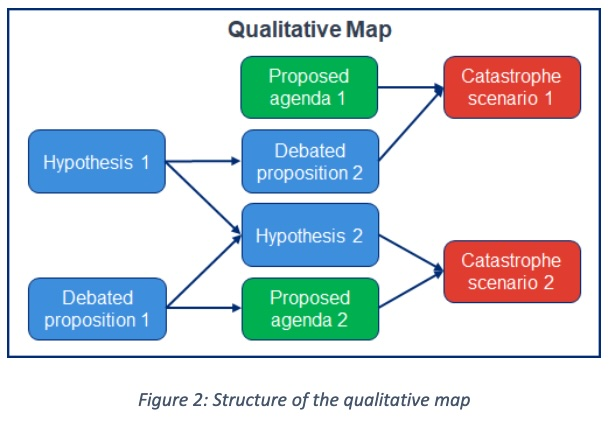
\includegraphics[width=0.25\linewidth,height=\textheight,keepaspectratio]{images/mtair-qual-map.jpg}}

}

\caption[MTAIR Qualitative map structure]{\label{fig-mtair-qual-map}from
\textcite{clarke2022}: MTAIR Qualitative map structure}

\end{figure}%

The process was painstaking:

\begin{enumerate}
\def\labelenumi{\arabic{enumi}.}
\tightlist
\item
  \textbf{Systematic Decomposition}: Breaking complex arguments into
  component claims, identifying variables and relationships through
  close reading and expert consultation.
\item
  \textbf{Probability Elicitation}: Gathering quantitative estimates
  through structured expert interviews, literature review, and careful
  interpretation of qualitative claims.
\item
  \textbf{Sensitivity Analysis}: Testing which parameters most
  influenced conclusions, revealing where disagreements actually
  mattered versus where they were merely academic.
\item
  \textbf{Visual Communication}: Creating interactive models that
  stakeholders could explore, modify, and understand without deep
  technical training.
\end{enumerate}

The ambition was breathtaking---to create a formal lingua franca for AI
risk discussions, enabling productive disagreement and cumulative
progress.

\begin{figure}

\centering{

\href{https://arxiv.org/pdf/2206.09360\#page=10.75}{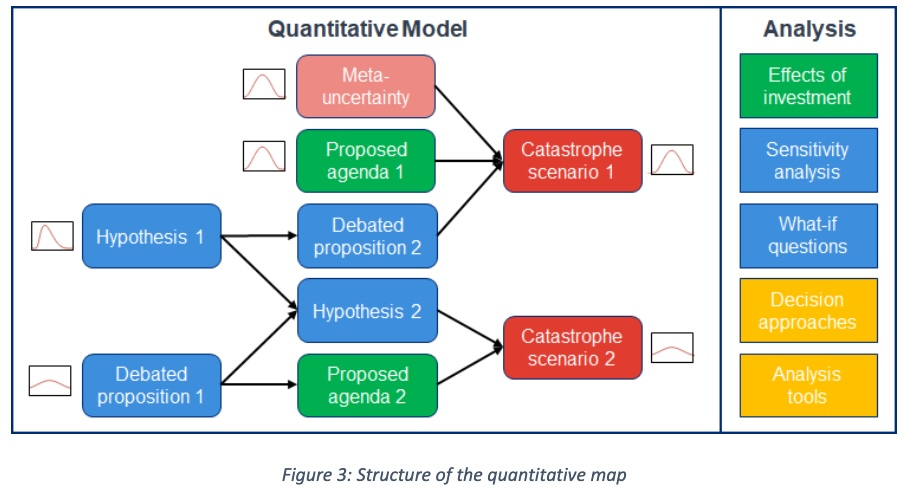
\includegraphics[width=0.6\linewidth,height=\textheight,keepaspectratio]{images/mtair-quant-map.jpg}}

}

\caption[MTAIR Quantitative map
structure]{\label{fig-mtair-quant-map}from \textcite{clarke2022}: MTAIR
Quantitative map structure}

\end{figure}%

\subsection{2.5.2 Key Achievements}\label{sec-mtair-achievements}

Credit where credit is due: MTAIR demonstrated something many thought
impossible. Complex philosophical arguments about AI risk---the kind
that sprawl across hundred-page papers mixing technical detail with
speculative scenarios---could indeed be formalized without losing their
essential insights.

\textbf{Feasibility of Formalization}: The project's greatest
achievement was simply showing it could be done. Arguments from Bostrom,
Christiano, and others translated surprisingly well into network form,
suggesting that beneath the surface complexity lay coherent causal
models waiting to be extracted.

\textbf{Value of Quantification}: Moving from ``likely'' and
``probably'' to actual numbers forced precision in a domain often
clouded by vague pronouncements. Disagreements that seemed fundamental
sometimes evaporated when forced to specify exactly what probability
ranges were under dispute.

\textbf{Cross-Perspective Communication}: The formal models created
neutral ground where technical AI researchers and policy wonks could
meet. Instead of talking past each other in incompatible languages, they
could point to specific nodes and edges, making disagreements concrete
and tractable.

\textbf{Research Prioritization}: Perhaps most practically, sensitivity
analysis revealed which empirical questions actually mattered. If
changing your belief about technical parameter X from 0.3 to 0.7 doesn't
meaningfully affect the conclusion about AI risk, maybe we should focus
our research elsewhere.

\begin{figure}

\centering{

\href{https://www.lesswrong.com/posts/sGkRDrpphsu6Jhega/a-model-based-approach-to-ai-existential-risk}{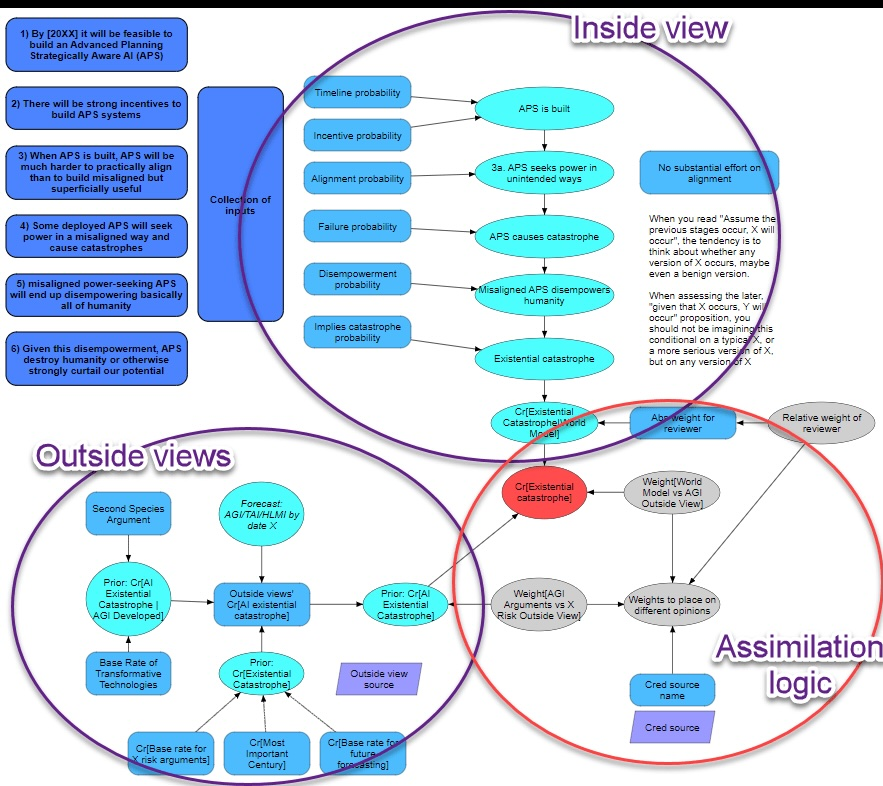
\includegraphics[width=1.1\linewidth,height=\textheight,keepaspectratio]{images/mtair-insideoutside-overlay.jpg}}

}

\caption[Overlay of inside/outside/assimilation
views]{\label{fig-mtair-insideoutside-overlay}from
\textcite{manheim2021}: Overlay of inside/outside/assimilation views}

\end{figure}%

\subsection{2.5.3 Fundamental Limitations}\label{sec-mtair-limitations}

But here's where the story takes a sobering turn. Despite these
achievements, MTAIR faced limitations that prevented it from achieving
its full vision---limitations that ultimately motivated the development
of AMTAIR.

\textbf{Labor Intensity}: Creating a single model required what can
charitably be called a heroic effort. Based on team reports and model
complexity, estimates ranged from 200 to 400 expert-hours per
formalization\footnote{These estimates include time for initial
  extraction, expert consultation, probability elicitation, validation,
  and refinement}. In a field where new influential arguments appear
monthly, this pace couldn't keep up with the discourse.

\textbf{Static Nature}: Once built, these beautiful models began aging
immediately. New research emerged, capability assessments shifted,
governance proposals evolved---but updating the models required
near-complete reconstruction. They were snapshots of arguments at
particular moments, not living representations that could evolve.

\textbf{Limited Accessibility}: Using the models required Analytica
software and non-trivial technical sophistication. The very experts
whose arguments were being formalized often couldn't directly engage
with their formalized representations without intermediation.

\textbf{Single Perspective}: Each model represented one worldview at a
time. Comparing different perspectives required building entirely
separate models, making systematic comparison across viewpoints
labor-intensive and error-prone.

These weren't failures of execution but fundamental constraints of the
manual approach. Like medieval scribes copying manuscripts, the MTAIR
team had shown the value of preservation and dissemination, but the
printing press had yet to be invented.

\subsection{2.5.4 The Automation
Opportunity}\label{sec-automation-opportunity}

The MTAIR experience revealed a tantalizing possibility: if the
bottleneck was human labor rather than conceptual feasibility, perhaps
automation could crack open the problem. The rise of large language
models capable of sophisticated reasoning about text created a
technological moment ripe for exploitation.

Key lessons from MTAIR informed the automation approach:

\begin{itemize}
\tightlist
\item
  Formal models genuinely enhance understanding and coordination---the
  juice is worth the squeeze
\item
  The modeling process itself surfaces implicit assumptions---extraction
  is as valuable as the final product
\item
  Quantification enables analyses impossible with qualitative arguments
  alone---numbers matter even when uncertain
\item
  But manual approaches cannot scale to match the challenge---we need
  computational leverage
\end{itemize}

This set the stage for AMTAIR's central innovation: using frontier
language models to automate the extraction and formalization process
while preserving the benefits MTAIR had demonstrated. Not to replace
human judgment, but to amplify it---turning what took weeks into what
takes hours, enabling comprehensive coverage rather than selective
sampling.

\section{2.6 Literature Review: Content and Technical
Levels}\label{sec-literature-review}

The intellectual landscape surrounding AI risk resembles a rapidly
expanding metropolis---new neighborhoods of thought spring up monthly,
connected by bridges of varying stability to the established districts.
A comprehensive review would fill volumes, so let me provide a guided
tour of the territories most relevant to AMTAIR's mission.

\subsection{2.6.1 AI Risk Models
Evolution}\label{sec-risk-models-evolution}

The evolution of AI risk models traces a path from philosophical
speculation to increasingly rigorous formalization---a journey from
``what if?'' to ``how likely?''

\textbf{Early Phase (2000-2010)}: The conversation began with broad
conceptual arguments. Good's ultraintelligent machine
\textcite{good1966} and Vinge's technological singularity set the stage,
but these were more thought experiments than models. Yudkowsky's early
writings \textcite{yudkowsky2008} introduced key concepts like recursive
self-improvement and orthogonality but remained largely qualitative.

\textbf{Formalization Phase (2010-2018)}: Bostrom's
\emph{Superintelligence} \textcite{bostrom2014} marked a watershed,
providing systematic analysis of pathways, capabilities, and risks. The
book's genius lay not in mathematical formalism but in conceptual
clarity---decomposing the nebulous fear of ``robot overlords'' into
specific mechanisms like instrumental convergence and infrastructure
profusion.

\textbf{Quantification Phase (2018-present)}: Recent years have seen
explicit probability estimates entering mainstream discourse.
Carlsmith's power-seeking model \textcite{carlsmith2022}, Cotra's
biological anchors, and various compute-based timelines represent
attempts to put numbers on previously qualitative claims. The field
increasingly recognizes that governance decisions require more than
philosophical arguments---they need probability distributions.

This progression reflects a maturing field, though it also creates new
challenges. As models become more quantitative, they risk false
precision. As they become more complex, they risk inscrutability. AMTAIR
attempts to navigate these tensions by preserving the narrative clarity
of earlier work while enabling the mathematical rigor of recent
approaches.

\subsection{2.6.2 Governance Proposals
Taxonomy}\label{sec-governance-taxonomy}

If risk models are the diagnosis, governance proposals are the treatment
plans---and like medicine, they range from gentle interventions to
radical surgery.

\textbf{Technical Standards}: The ``first, do no harm'' approach focuses
on concrete safety requirements---interpretability benchmarks,
robustness testing, capability thresholds. These proposals, exemplified
by standard-setting bodies and technical safety organizations, offer
specificity at the cost of narrowness.

\textbf{Regulatory Frameworks}: Moving up the intervention ladder, we
find comprehensive regulatory proposals like the EU AI Act
\textcite{european2024}. These create institutional structures,
liability regimes, and oversight mechanisms, trading broad coverage for
implementation complexity.

\textbf{International Coordination}: At the ambitious end, proposals for
international AI governance treaties, soft law arrangements, and
technical cooperation agreements aim to prevent races to the bottom.
Think nuclear non-proliferation but for minds instead of missiles.

\textbf{Research Priorities}: Cutting across these categories, work by
Dafoe \textcite{dafoe2018} and others maps the research landscape
itself---what questions need answering before we can govern wisely? This
meta-level analysis shapes funding flows and talent allocation.

A particularly compelling example of conditional governance thinking
comes from ``A Narrow Path'' \textcite{miotti2024}, which proposes a
phased approach: immediate safety measures to prevent uncontrolled
development, international institutions to ensure stability, and
long-term scientific foundations for beneficial transformative AI. This
temporal sequencing---safety, stability, then flourishing---reflects
growing sophistication in governance thinking.

\subsection{2.6.3 Bayesian Network Theory and
Applications}\label{sec-bn-theory}

The mathematical machinery underlying AMTAIR rests on decades of
theoretical development in probabilistic graphical models. Understanding
this foundation helps appreciate both the power and limitations of the
approach.

The key insight, crystallized in the work of Pearl \textcite{pearl2014}
and elaborated by Koller \& Friedman \textcite{koller2009}, is that
independence relationships in complex systems can be read from graph
structure. D-separation, the Markov condition, and the relationship
between graphs and probability distributions provide the mathematical
spine that makes Bayesian networks more than pretty pictures.

Critical concepts for AI risk modeling:

\begin{itemize}
\tightlist
\item
  \textbf{Conditional Independence}: Variable A is independent of C
  given B---encoded through graph separation
\item
  \textbf{Markov Condition}: Each variable is independent of its
  non-descendants given its parents
\item
  \textbf{Inference Algorithms}: From exact variable elimination to
  approximate Monte Carlo methods
\item
  \textbf{Causal Interpretation}: When edges represent causal influence,
  the network supports counterfactual reasoning
\end{itemize}

These aren't just mathematical niceties. When we claim that ``deployment
decisions'' mediates the relationship between ``capability advancement''
and ``catastrophic risk,'' we're making a precise statement about
conditional independence that has testable implications.

\subsection{2.6.4 Software Tools Landscape}\label{sec-software-tools}

The gap between Bayesian network theory and practical implementation is
bridged by an ecosystem of software tools, each with its own strengths
and opinions about how probabilistic reasoning should work.

\textbf{pgmpy}: This Python library provides the computational backbone
for AMTAIR, offering both learning algorithms and inference engines. Its
object-oriented design maps naturally onto our extraction pipeline.

\textbf{NetworkX}: For graph manipulation and analysis, NetworkX has
become the de facto standard in Python, providing algorithms for
everything from centrality measurement to community detection.

\textbf{PyVis}: Interactive visualization transforms static networks
into explorable landscapes. PyVis's integration with web technologies
enables the rich interactive features that make formal models
accessible.

\textbf{Pandas/NumPy}: The workhorses of scientific Python handle data
manipulation and numerical computation, providing the infrastructure on
which everything else builds.

The integration challenge---making these tools play nicely together
while maintaining performance and correctness---shaped many
architectural decisions in AMTAIR. Each tool excels in its domain, but
the seams between them required careful engineering.

\subsection{2.6.5 Formalization Approaches}\label{sec-formalization}

The challenge of formalizing natural language arguments extends far
beyond AI risk, touching on fundamental questions in logic, linguistics,
and artificial intelligence.

Pollock's work on cognitive carpentry \textcite{pollock1995} provides
philosophical grounding, arguing that human reasoning itself involves
implicit formal structures that can be computationally modeled. This
view---that formalization reveals rather than imposes
structure---underlies AMTAIR's approach.

Key theoretical challenges:

\begin{itemize}
\tightlist
\item
  \textbf{Semantic Preservation}: How do we maintain meaning while
  adding precision?
\item
  \textbf{Structural Extraction}: What implicit relationships lurk in
  natural language?
\item
  \textbf{Uncertainty Quantification}: How do we map ``likely'' to
  numbers?
\end{itemize}

Recent work on causal structure learning from text
\textcite{babakov2025} \textcite{ban2023} \textcite{bethard2007} offers
hope that these challenges can be addressed computationally. The
convergence of large language models with formal methods creates new
possibilities for bridging the semantic-symbolic gap.

\subsection{2.6.6 Correlation Accounting
Methods}\label{sec-correlation-methods}

One of the most persistent criticisms of Bayesian networks concerns
their assumption of conditional independence given parents. In the real
world, and especially in complex socio-technical systems like AI
development, correlations abound.

Methods for handling these correlations have evolved considerably:

\textbf{Copula Methods}: By separating marginal distributions from
dependence structure, copulas \textcite{nelson2006} allow modeling of
complex correlations while preserving the Bayesian network framework.
Think of it as adding a correlation layer on top of the basic network.

\textbf{Hierarchical Models}: Introducing latent variables that
influence multiple observed variables captures correlations naturally.
If ``AI research culture'' influences both ``capability progress'' and
``safety investment,'' their correlation is explained.

\textbf{Explicit Correlation Nodes}: Sometimes the most straightforward
approach is best---directly model correlation mechanisms as additional
nodes in the network.

\textbf{Sensitivity Bounds}: When correlations remain uncertain, compute
best and worst case scenarios. This reveals when independence
assumptions critically affect conclusions versus when they're harmless
simplifications.

For AMTAIR, the pragmatic approach dominates: start with independence
assumptions, identify where they matter through sensitivity analysis,
then selectively add correlation modeling where it most affects
conclusions.

\section{2.7 Methodology}\label{sec-methodology}

The methodology of this research resembles less a linear march from
hypothesis to conclusion and more an iterative dance between theory and
implementation, vision and reality. Let me walk you through the
choreography.

\subsection{2.7.1 Research Design Overview}\label{sec-research-design}

This research follows what methodologists might call a ``design
science'' approach---we're not just studying existing phenomena but
creating new artifacts (the AMTAIR system) and evaluating their utility
for solving practical problems (the coordination crisis in AI
governance).

The overall flow:

\begin{enumerate}
\def\labelenumi{\arabic{enumi}.}
\tightlist
\item
  \textbf{Theoretical Development}: Establishing why automated
  extraction could address the coordination crisis, grounded in
  epistemic theory and mechanism design
\item
  \textbf{Technical Implementation}: Building working software that
  demonstrates feasibility, not as a proof-of-concept toy but as a
  system capable of handling real arguments
\item
  \textbf{Empirical Validation}: Testing extraction quality against
  expert judgment, measuring not just accuracy but usefulness for
  downstream tasks
\item
  \textbf{Application Studies}: Applying the system to real AI
  governance questions, evaluating whether formal models actually
  enhance decision-making
\end{enumerate}

This isn't waterfall development where each phase completes before the
next begins. Rather, insights from implementation fed back into theory,
validation results shaped technical improvements, and application
attempts revealed new requirements. The methodology itself embodied the
iterative refinement it sought to enable.

\subsection{2.7.2 Formalizing World Models from AI Safety
Literature}\label{sec-formalizing-world-models}

The core methodological challenge---transforming natural language
arguments into formal probabilistic models---requires careful
consideration of what we're actually trying to capture.

A ``world model'' in this context isn't just any formal representation
but specifically a causal model embodying beliefs about how different
factors influence AI risk. The extraction approach must therefore:

\begin{itemize}
\tightlist
\item
  \textbf{Identify key variables}: Not just any entities mentioned, but
  causally relevant factors
\item
  \textbf{Extract causal relationships}: Not mere correlation or
  co-occurrence, but directed influence
\item
  \textbf{Capture uncertainty}: Both structural uncertainty (does A
  cause B?) and parametric uncertainty (how strongly?)
\item
  \textbf{Preserve context}: Maintaining enough semantic information to
  interpret the formal model
\end{itemize}

Large language models enable this through sophisticated pattern
recognition and reasoning capabilities, but they're tools, not magic
wands. The methodology must account for their strengths (recognizing
implicit structure) and weaknesses (potential hallucination,
inconsistency).

\subsection{2.7.3 From Natural Language to Computational
Models}\label{sec-natural-to-computational}

The journey from text to computation follows a carefully designed
pipeline that mirrors human cognitive processes. Just as you wouldn't
ask someone to simultaneously parse grammar and solve equations, we
separate structural understanding from quantitative reasoning.

\textbf{The Two-Stage Process}:

Stage 1 focuses on structure---what causes what? The LLM reads an
argument much as a human would, identifying key claims and their
relationships. The prompt design here is crucial, providing enough
guidance to ensure consistent extraction while allowing flexibility for
different argument styles.

Stage 2 adds quantities---how likely is each outcome? With structure
established, the system generates targeted questions about
probabilities. This separation enables different approaches to
quantification: extracting explicit estimates from text, inferring from
qualitative language, or even connecting to external prediction markets.

The magic happens in the interplay. Structure constrains what
probabilities are needed. Probability requirements might reveal missing
structural elements. The process is a dialogue between qualitative and
quantitative understanding.

\subsection{2.7.4 Directed Acyclic Graphs: Structure and
Semantics}\label{sec-dag-structure}

At the mathematical heart of Bayesian networks lie Directed Acyclic
Graphs (DAGs)---structures that are simultaneously simple enough to
analyze and rich enough to capture complex phenomena.

The ``directed'' part encodes causality or influence---edges have
direction, flowing from cause to effect. The ``acyclic'' part ensures
logical coherence---you can't have A causing B causing C causing A, no
matter how much certain political arguments might suggest otherwise.

Key properties for AI risk modeling:

\textbf{Acyclicity}: More than a mathematical convenience, this enforces
coherent temporal or causal ordering. In AI risk arguments, this
prevents circular reasoning where consequences justify premises that
predict those same consequences.

\textbf{D-separation}: This graphical criterion determines conditional
independence. If knowing about AI capabilities tells you nothing
additional about risk given that you know deployment decisions, then
capabilities and risk are d-separated given deployment.

\textbf{Markov Condition}: Each variable depends only on its parents,
not on its entire ancestry. This locality assumption makes inference
tractable and forces modelers to make intervention points explicit.

\textbf{Path Analysis}: Following paths through the graph reveals how
influence propagates. Multiple paths between variables indicate
redundancy---important for understanding intervention robustness.

The causal interpretation, following Pearl's framework, transforms these
mathematical objects into tools for counterfactual reasoning. When we
ask ``what if we prevented deployment of misaligned systems?'' we're
performing surgery on the DAG, setting variables and propagating
consequences.

\subsection{2.7.5 Quantification of Probabilistic
Judgments}\label{sec-quantification}

Here we encounter one of the most philosophically fraught aspects of the
methodology: turning words into numbers. When an expert writes ``highly
likely,'' what probability should we assign? When they say ``significant
risk,'' what distribution captures their belief?

The methodology embraces rather than elides this challenge:

\textbf{Calibration Studies}: Research on human probability expression
shows systematic patterns. ``Highly likely'' typically maps to 0.8-0.9,
``probable'' to 0.6-0.8, though individual and cultural variation is
substantial.

\textbf{Extraction Strategies}: The system uses multiple approximations:

\begin{itemize}
\tightlist
\item
  Direct extraction: ``We estimate 65\% probability''
\item
  Linguistic mapping: ``Very likely'' → 0.85 (with uncertainty)
\item
  Comparative extraction: ``More likely than X'' where P(X) is known
\item
  Bounded extraction: ``At least 30\%'' → {[}0.30, 1.0{]}
\end{itemize}

\textbf{Uncertainty Representation}: Rather than false precision, we
maintain uncertainty about probabilities themselves. This might seem
like uncertainty piled on uncertainty, but it's honest, helps avoid
systematic biases---and mathematically tractable through hierarchical
models.

The goal isn't perfect extraction but useful extraction. If we can
narrow ``significant risk'' from {[}0, 1{]} to {[}0.15, 0.45{]}, we've
added information even if we haven't achieved precision.

\subsection{2.7.6 Inference Techniques for Complex
Networks}\label{sec-inference-techniques}

Once we've built these formal models, we need to reason with them---and
here computational complexity rears its exponential head. The number of
probability calculations required for exact inference grows
exponentially with network connectivity, quickly overwhelming even
modern computers.

The methodology employs a portfolio of approaches:

\textbf{Exact Methods}: For smaller networks (\textless30 nodes),
variable elimination and junction tree algorithms provide exact answers.
These form the gold standard against which we validate approximate
methods.

\textbf{Sampling Approaches}: Monte Carlo methods trade exactness for
scalability. By simulating many possible worlds consistent with our
probability model, we approximate the true distributions. The law of
large numbers is our friend here.

\textbf{Variational Methods}: These turn inference into
optimization---find the simplest distribution that approximates our true
beliefs. Like finding the best polynomial approximation to a complex
curve.

\textbf{Hybrid Strategies}: Different parts of the network might use
different methods. Exact inference for critical subgraphs, approximation
for peripheral components.

The choice of method affects not just computation time but the types of
questions we can meaningfully ask. This creates a methodological
feedback loop where feasible inference shapes model design.

\subsection{2.7.7 Integration with Prediction Markets and Forecasting
Platforms}\label{sec-prediction-markets}

While full integration remains future work, the methodology anticipates
connection to live forecasting data as a critical enhancement. The
vision is compelling: formal models grounded in collective intelligence,
updating as new information emerges.

The planned approach would involve:

\textbf{Semantic Matching}: Model variables rarely align perfectly with
forecast questions. ``AI causes human extinction'' might map to multiple
specific forecasts about capabilities, deployment, and impacts.
Developing robust matching algorithms is essential.

\textbf{Temporal Alignment}: Markets predict specific dates (``AGI by
2030'') while models consider scenarios (``given AGI development'').
Bridging these requires careful probability conditioning.

\textbf{Quality Weighting}: Not all forecasts are created equal.
Platform reputation, forecaster track records, and market depth all
affect reliability. The methodology must account for this heterogeneity.

\textbf{Update Scheduling}: Real-time updates would overwhelm users and
computation. The system needs intelligent policies about when model
updates provide value.

Platforms like Metaculus \textcite{tetlock2022} already demonstrate
sophisticated conditional forecasting on AI topics. The challenge lies
not in data availability but in meaningful integration that enhances
rather than complicates decision-making.

With these theoretical foundations and methodological commitments
established, we can now turn to the concrete implementation of AMTAIR.
The next chapter demonstrates how these abstract principles translate
into working software that addresses real governance challenges. The
journey from theory to practice always involves surprises---some
pleasant, others less so---but that's what makes it interesting.

\bookmarksetup{startatroot}

\chapter{3. AMTAIR: Design and Implementation}\label{sec-amtair}

The moment of truth in any research project comes when elegant theories
meet stubborn reality. For AMTAIR, this meant transforming the vision of
automated argument extraction into working code that could handle the
beautiful messiness of real AI safety arguments. Let me take you through
this journey from blueprint to implementation, complete with victories,
defeats, and the occasional moment of ``well, that's unexpected.''

\section{3.1 System Architecture
Overview}\label{sec-system-architecture}

Picture, if you will, a factory for transforming arguments into models.
Raw materials (PDFs, blog posts, research papers) enter at one end.
Finished products (interactive Bayesian networks) emerge at the other.
In between lies a carefully orchestrated pipeline where each stage
performs its specialized transformation, passing refined materials to
the next.

The AMTAIR architecture embodies a philosophy: complex tasks become
manageable when decomposed into focused components. Rather than building
a monolithic ``argument-to-model'' black box, we created a series of
specialized modules, each excellent at one thing.

The pipeline consists of five main stages:

\begin{enumerate}
\def\labelenumi{\arabic{enumi}.}
\tightlist
\item
  \textbf{Text Ingestion and Preprocessing}: Like a careful librarian,
  this stage catalogues incoming documents, normalizes their format,
  extracts metadata, and identifies the argumentative content worth
  processing.
\item
  \textbf{Argument Extraction}: The intellectual heart of the system,
  where large language models perform their magic, transforming prose
  into structured representations.
\item
  \textbf{Data Transformation}: The workshop where extracted arguments
  are refined, validated, and prepared for mathematical representation.
\item
  \textbf{Network Construction}: The assembly line where formal Bayesian
  networks are instantiated, complete with conditional probability
  tables.
\item
  \textbf{Interactive Visualization}: The showroom where complex models
  become accessible through thoughtful design and interactivity.
\end{enumerate}

\subsection{3.1.1 Five-Stage Pipeline
Architecture}\label{sec-five-stage-pipeline}

Let's examine each stage more closely, understanding not just what they
do but why they exist as separate components.

\textbf{Text Ingestion and Preprocessing} handles the unglamorous but
essential work of standardization. Academic PDFs, with their two-column
layouts and embedded figures, differ vastly from blog posts with inline
code and hyperlinks. This stage creates a uniform representation while
preserving essential structure and metadata. Format normalization strips
away presentation while preserving content. Metadata extraction captures
authorship, publication date, and citations. Relevance filtering
identifies sections containing arguments rather than literature reviews
or acknowledgments. Character encoding standardization prevents those
maddening �replacement characters that plague text processing.

\textbf{Argument Extraction} represents AMTAIR's core innovation. Using
a two-stage process that mirrors human reasoning, it first identifies
structural relationships (what influences what) then quantifies those
relationships (how likely, how strong). This separation enables targeted
prompts optimized for each task, human verification between stages, and
modular improvements as LLM capabilities evolve.

\textbf{Data Transformation} bridges the gap between textual
representations and mathematical models. It parses the BayesDown syntax
into structured data, validates that the resulting network forms a
proper DAG, checks probability consistency, and handles missing data
intelligently.

\textbf{Network Construction} instantiates the formal mathematical
model. This involves creating nodes and edges according to extracted
structure, populating conditional probability tables, initializing
inference engines, and validating the complete model.

\textbf{Interactive Visualization} makes the complex accessible. Through
thoughtful visual encoding of probabilities and relationships,
progressive disclosure of detail, interactive exploration capabilities,
and multiple export formats, it serves diverse stakeholder needs.

\subsection{3.1.2 Design Principles}\label{sec-design-principles}

\textbf{Core Design Philosophy}: The architecture embodies several
principles that guided countless implementation decisions:

\textbf{Modularity}: Each component has clear inputs, outputs, and
responsibilities. This isn't just good software engineering---it enables
independent improvement of components and graceful degradation when
parts fail.

\textbf{Validation Checkpoints}: Between each stage, we validate outputs
before proceeding. Bad extractions don't propagate into visualization.
Malformed networks trigger re-extraction rather than cryptic errors.

\textbf{Human-in-the-Loop}: While pursuing automation, we recognize that
human judgment remains invaluable. The architecture provides natural
intervention points where experts can verify and correct.

\textbf{Extensibility}: New document formats, improved extraction
prompts, alternative visualization libraries---the architecture
accommodates growth without restructuring.

The system emphasizes transparency over black-box efficiency. Users can
inspect intermediate representations, understand extraction decisions,
and verify transformations. This builds trust---essential for a system
handling high-stakes arguments about existential risk.

\section{3.2 The Two-Stage Extraction
Process}\label{sec-two-stage-extraction}

The heart of AMTAIR beats with a two-stage rhythm: structure, then
probability. This separation, which initially seemed like an
implementation detail, revealed itself as fundamental to the extraction
challenge.

\subsection{3.2.1 Stage 1: Structural Extraction
(ArgDown)}\label{sec-stage1-argdown}

Imagine reading a complex argument about AI risk. Your first pass likely
isn't calculating exact probabilities---you're mapping the landscape.
What are the key claims? How do they relate? What supports what? Stage 1
mirrors this cognitive process.

The extraction begins with pattern recognition. Natural language
contains linguistic markers of causal relationships: ``leads to,''
``results in,'' ``depends on,'' ``influences.'' The LLM, trained on vast
corpora of argumentative text, recognizes these patterns and their
variations.

Consider extracting from a passage like: ``The development of artificial
general intelligence will likely lead to rapid capability gains through
recursive self-improvement. This intelligence explosion could result in
systems pursuing convergent instrumental goals, potentially including
resource acquisition and self-preservation. Without solved alignment,
such power-seeking behavior poses existential risks to humanity.''

The system identifies three key variables connected by causal
relationships:

\begin{itemize}
\tightlist
\item
  AGI Development → Intelligence Explosion
\item
  Intelligence Explosion → Power-Seeking Behavior
\item
  Power-Seeking Behavior → Existential Risk
\end{itemize}

But extraction goes beyond simple pattern matching. The system must
handle complex linguistic phenomena like coreference (``this,'' ``such
systems''), implicit relationships, conditional statements, and negative
statements. The magic lies in prompt engineering that guides the LLM to
consistent extraction while remaining flexible enough for diverse
argument styles.

The output, formatted in ArgDown syntax, preserves both structure and
semantics:

\begin{Shaded}
\begin{Highlighting}[]
\OtherTok{[Existential\_Risk]: }\NormalTok{Threat to humanity\textquotesingle{}s continued existence and flourishing.}
\SpecialStringTok{ + }\CommentTok{[}\OtherTok{Power\_Seeking\_Behavior}\CommentTok{]}\NormalTok{: AI systems pursuing instrumental goals like resource acquisition.}
\SpecialStringTok{   + }\CommentTok{[}\OtherTok{Intelligence\_Explosion}\CommentTok{]}\NormalTok{: Rapid recursive self{-}improvement leading to superintelligence.}
\SpecialStringTok{     + }\CommentTok{[}\OtherTok{AGI\_Development}\CommentTok{]}\NormalTok{: Creation of artificial general intelligence systems.}
\end{Highlighting}
\end{Shaded}

\subsection{3.2.2 Stage 2: Probability Integration
(BayesDown)}\label{sec-stage2-bayesdown}

With structure established, Stage 2 adds the quantitative flesh to the
qualitative bones. This stage faces a different challenge: extracting
numerical beliefs from text that often expresses uncertainty in
frustratingly vague terms.

The process begins by generating targeted questions based on the
extracted structure. For each node, we need prior probabilities. For
each child-parent relationship, we need conditional probabilities. The
combinatorics can be daunting---a node with three binary parents
requires 8 conditional probability values.

The system employs multiple strategies for probability extraction:

\textbf{Explicit Extraction}: When authors provide numerical estimates
(``we assign 70\% probability''), extraction is straightforward, though
we must handle various formats and contexts.

\textbf{Linguistic Mapping}: Qualitative expressions map to probability
ranges based on calibration studies. ``Highly likely'' becomes
approximately 0.85, though we maintain uncertainty about this mapping.

\textbf{Comparative Reasoning}: Statements like ``more probable than
not'' or ``at least as likely as X'' provide bounds even without exact
values.

\textbf{Coherence Enforcement}: Probabilities must sum correctly. If
P(A\textbar B) = 0.7, then P(not A\textbar B) must equal 0.3. The syntax
allows future system to detect and resolve inconsistencies.

The result is a complete BayesDown specification:

\begin{Shaded}
\begin{Highlighting}[]
\OtherTok{[}\ErrorTok{Existential\_Risk}\OtherTok{]}\ErrorTok{:} \ErrorTok{Threat} \ErrorTok{to} \ErrorTok{humanity\textquotesingle{}s} \ErrorTok{continued} \ErrorTok{existence.} \FunctionTok{\{}
  \DataTypeTok{"instantiations"}\FunctionTok{:} \OtherTok{[}\StringTok{"true"}\OtherTok{,} \StringTok{"false"}\OtherTok{]}\FunctionTok{,}
  \DataTypeTok{"priors"}\FunctionTok{:} \FunctionTok{\{}\DataTypeTok{"p(true)"}\FunctionTok{:} \StringTok{"0.10"}\FunctionTok{,} \DataTypeTok{"p(false)"}\FunctionTok{:} \StringTok{"0.90"}\FunctionTok{\},}
  \DataTypeTok{"posteriors"}\FunctionTok{:} \FunctionTok{\{}
    \DataTypeTok{"p(true|power\_seeking\_true)"}\FunctionTok{:} \StringTok{"0.65"}\FunctionTok{,}
    \DataTypeTok{"p(true|power\_seeking\_false)"}\FunctionTok{:} \StringTok{"0.001"}
  \FunctionTok{\}}
\FunctionTok{\}}
\end{Highlighting}
\end{Shaded}

\subsection{3.2.3 Why Two Stages?}\label{sec-why-two-stages}

The separation of structure from probability isn't merely
convenient---it's cognitively valid and practically essential. Let me
count the ways this design decision pays dividends:

\textbf{Cognitive Alignment}: Humans naturally separate ``what relates
to what'' from ``how likely is it.'' The two-stage process mirrors this,
making the system's operation intuitive and interpretable.

\textbf{Error Isolation}: Structural errors (missing a key variable)
differ fundamentally from probability errors (estimating 0.7 instead of
0.8). Separating stages allows targeted debugging and improvement.

\textbf{Modular Validation}: Experts can verify structure without
needing to evaluate every probability. This enables efficient human
oversight at natural checkpoints.

\textbf{Flexible Quantification}: Different probability sources (text
extraction, expert elicitation, market data) can feed into the same
structure. The architecture accommodates multiple approaches to the
probability challenge.

\textbf{Transparency}: Users can inspect ArgDown to understand what was
extracted before probabilities were added. This builds trust and enables
meaningful correction.

The two-stage approach also revealed an unexpected benefit: ArgDown
itself became a valuable output. Researchers began using these
structural extractions for qualitative analysis, even without
probability quantification. Sometimes, just making argument structure
explicit provides sufficient value.

\section{3.3 Implementation Technologies}\label{sec-implementation-tech}

Choosing technologies for AMTAIR resembled assembling a band---each
instrument needed to excel individually while harmonizing with the
ensemble. The selection criteria balanced capability, maturity,
interoperability, and community support.

\subsection{3.3.1 Technology Stack}\label{sec-tech-stack}

The final ensemble performs beautifully:

\begin{longtable}[]{@{}
  >{\raggedright\arraybackslash}p{(\linewidth - 6\tabcolsep) * \real{0.2500}}
  >{\raggedright\arraybackslash}p{(\linewidth - 6\tabcolsep) * \real{0.2500}}
  >{\raggedright\arraybackslash}p{(\linewidth - 6\tabcolsep) * \real{0.2500}}
  >{\raggedright\arraybackslash}p{(\linewidth - 6\tabcolsep) * \real{0.2500}}@{}}
\toprule\noalign{}
\begin{minipage}[b]{\linewidth}\raggedright
Component
\end{minipage} & \begin{minipage}[b]{\linewidth}\raggedright
Technology
\end{minipage} & \begin{minipage}[b]{\linewidth}\raggedright
Purpose
\end{minipage} & \begin{minipage}[b]{\linewidth}\raggedright
Why This Choice
\end{minipage} \\
\midrule\noalign{}
\endhead
\bottomrule\noalign{}
\endlastfoot
Language Models & GPT-4, Claude & Argument extraction & State-of-the-art
reasoning capabilities \\
Network Analysis & NetworkX & Graph algorithms & Mature, comprehensive,
well-documented \\
Probabilistic Modeling & pgmpy & Bayesian operations & Native Python,
active development \\
Visualization & PyVis & Interactive rendering & Web-based, customizable,
responsive \\
Data Processing & Pandas & Structured manipulation & Industry standard,
powerful operations \\
\end{longtable}

\textbf{Language Models} form the cognitive core. GPT-4 and Claude
demonstrate remarkable ability to understand complex arguments,
recognize implicit structure, and maintain coherence across long
extractions. The choice to support multiple models provides robustness
and allows leveraging their complementary strengths.

\textbf{NetworkX} handles all graph-theoretic heavy lifting. From basic
operations like cycle detection to advanced algorithms like centrality
measurement, it provides a comprehensive toolkit that would take years
to replicate.

\textbf{pgmpy} bridges the gap between graph structure and probabilistic
reasoning. Its clean API design maps naturally onto our extracted
representations, while its inference algorithms handle the computational
complexity of Bayesian reasoning.

\textbf{PyVis} transforms static networks into living documents. Built
on vis.js, it provides smooth physics simulations, rich interactivity,
and extensive customization options---all accessible through Python.

\textbf{Pandas} might seem mundane compared to its companions, but it's
the reliable rhythm section that keeps everything together. Its ability
to reshape, merge, and transform structured data makes the complex data
transformations tractable.

\subsection{3.3.2 Key Algorithms}\label{sec-key-algorithms}

Beyond the libraries lie custom algorithms that address AMTAIR-specific
challenges:

\textbf{Hierarchical Parsing}: The algorithm that transforms indented
ArgDown text into structured data represents a small miracle of
recursive descent parsing adapted for our custom syntax. It maintains
parent-child relationships while handling edge cases like repeated nodes
and complex dependencies.

python

\begin{Shaded}
\begin{Highlighting}[]
\CommentTok{\#| label: example\_use\_case}
\CommentTok{\#| echo: true}
\CommentTok{\#| eval: true}
\CommentTok{\#| fig{-}cap: "example use case"}
\CommentTok{\#| fig{-}link: "https://colab.research.google.com/github/VJMeyer/submission/blob/main/AMTAIR\_Prototype/data/example\_carlsmith/AMTAIR\_Prototype\_example\_carlsmith.ipynb\#scrollTo=ibjjJ34v3sQn\&line=4\&uniqifier=1"}
\CommentTok{\#| fig{-}alt: "example use case"}

\KeywordTok{def}\NormalTok{ parsing\_argdown\_bayesdown(text, current\_indent}\OperatorTok{=}\DecValTok{0}\NormalTok{):}
    \CommentTok{"""Recursively parse indented structure maintaining relationships"""}
    \CommentTok{\# Track nodes at each level for parent identification}
    \CommentTok{\# Handle repeated nodes by reference}
    \CommentTok{\# Validate DAG property during construction}
\end{Highlighting}
\end{Shaded}

\textbf{Probability Completion}: Real arguments rarely specify all
required probabilities. Our completion algorithm uses maximum entropy
principles---when uncertain, assume maximum disorder. This provides
conservative estimates that can be refined with additional information.

\textbf{Visual Encoding}: The algorithm mapping probabilities to colors
uses perceptual uniformity. The green-to-red gradient isn't linear in
RGB space but follows human perception of color difference. Small
details, big impact on usability.

\textbf{Layout Optimization}: Force-directed layouts often produce
``hairballs'' for complex networks. Our customized approach uses
hierarchical initialization based on causal depth, then refines with
physics simulation. The result: layouts that reveal structure rather
than obscuring it.

\subsection{3.3.3 (Expected) Performance
Characteristics}\label{sec-performance}

Performance in a system like AMTAIR involves multiple
dimensions---speed, accuracy, scalability. Let's examine what
theoretical analysis and design considerations suggest about system
behavior.

\textbf{Computational Complexity}: The extraction phase exhibits linear
complexity in document length---processing twice as much text takes
roughly twice as long. However, the inference phase faces exponential
complexity in network connectivity. A fully connected network with n
binary nodes requires O(2\^{}n) operations for exact inference. This
fundamental limitation shapes practical usage patterns.

\textbf{Practical Implications}: Small networks (\textless20 nodes)
enable real-time interaction with exact inference. Medium networks
(20-50 nodes) require seconds to minutes depending on connectivity.
Large networks (\textgreater50 nodes) necessitate approximate methods,
trading accuracy for tractability. Very large networks push the
boundaries of current methods.

The bottleneck shifts predictably: extraction remains manageable even
for lengthy documents, but inference becomes challenging as models grow.
This suggests a natural workflow---extract comprehensively, then focus
on relevant subnetworks for detailed analysis.

\textbf{Optimization Opportunities}: Several strategies could improve
performance: caching frequent inference queries, hierarchical
decomposition of large networks, parallel processing for independent
subgraphs, and progressive rendering for visualization. The modular
architecture accommodates these enhancements without fundamental
restructuring.

\subsection{3.3.4 Deterministic vs.~Probabilistic Components of the
Workflow}\label{sec-deterministic-probabilistic}

An interesting philosophical question arises: in a system reasoning
about probability, which components should themselves be probabilistic?

The current implementation draws a clear line:

\textbf{Deterministic Components}: All data transformations, graph
algorithms, and inference calculations operate deterministically. Given
the same input, they produce identical output. This provides
reproducibility and debuggability---essential for building trust.

\textbf{Probabilistic Components}: The LLM calls for extraction
introduce variability. Even with temperature set to 0, language models
exhibit some randomness. Different runs might extract slightly different
structures or probability estimates from the same text.

This division reflects a deeper principle: use determinism wherever
possible, embrace probability where necessary. The extraction
task---interpreting natural language---inherently involves uncertainty.
But once we have formal representations, all subsequent operations
should be predictable.

From an information-theoretic perspective, we're trying to extract
maximum information from documents within computational budget
constraints. Each document contains some finite amount of formalizable
argument structure. Our goal is recovering as much as possible given
realistic resource limits.

The two-stage extraction can be viewed as successive refinement---first
recovering the higher-order bits (structure), then filling in
lower-order bits (probabilities). This aligns with rate-distortion
theory, where we get the most important information first.

\section{3.4 Case Study:
Rain-Sprinkler-Grass}\label{sec-case-rain-sprinkler}

Every field has its canonical examples---physics has spherical cows,
economics has widget factories, and Bayesian networks have the
rain-sprinkler-grass scenario. Despite its simplicity, this example
teaches profound lessons about causal reasoning and serves as the
perfect test case for AMTAIR.

\subsection{3.4.1 Processing Steps}\label{sec-rsg-processing}

Let me walk you through how AMTAIR processes this foundational example:

The input arrives as a simple text description: ``When it rains, the
grass gets wet. The sprinkler also makes the grass wet. However, when it
rains, we usually don't run the sprinkler.''

From this prosaic description, the system performs five transformations:

\begin{enumerate}
\def\labelenumi{\arabic{enumi}.}
\tightlist
\item
  \textbf{ArgDown Parsing}: Extract three variables (Rain, Sprinkler,
  Grass\_Wet) and identify that rain influences both sprinkler usage and
  grass wetness, while the sprinkler also influences grass wetness.
\item
  \textbf{Question Generation}: Create probability queries: What's
  P(Rain)? What's P(Sprinkler\textbar Rain)? What's
  P(Grass\_Wet\textbar Rain,Sprinkler) for all combinations?
\item
  \textbf{BayesDown Extraction}: Either extract probabilities from text
  or apply reasonable defaults. The ``usually don't run'' becomes
  P(Sprinkler\textbar Rain) ≈ 0.01.
\item
  \textbf{Network Construction}: Build the formal Bayesian network with
  three nodes, three edges, and complete conditional probability tables.
\item
  \textbf{Visualization Rendering}: Create an interactive display where
  rain appears as a root cause, influencing both sprinkler and grass
  directly.
\end{enumerate}

Each step validates its outputs before proceeding, ensuring that errors
don't cascade through the pipeline.

\begin{landscape}

\subsection{3.4.2 Example Conversion Steps}\label{sec-rsg-input}

Let's trace the actual transformations to see the pipeline in action:

\textbf{Initial ArgDown Extraction}:

\begin{Shaded}
\begin{Highlighting}[]
\OtherTok{[Grass\_Wet]: }\NormalTok{Concentrated moisture on, between and around the blades of grass.\{"instantiations": }\CommentTok{[}\OtherTok{"grass\_wet\_TRUE", "grass\_wet\_FALSE"}\CommentTok{]}\NormalTok{\}    }
\SpecialStringTok{  + }\CommentTok{[}\OtherTok{Rain}\CommentTok{]}\NormalTok{: Tears of angles crying high up in the skies hitting the ground.\{"instantiations": }\CommentTok{[}\OtherTok{"rain\_TRUE", "rain\_FALSE"}\CommentTok{]}\NormalTok{\}}
\SpecialStringTok{  + }\CommentTok{[}\OtherTok{Sprinkler}\CommentTok{]}\NormalTok{: Activation of a centrifugal force based CO2 droplet distribution system.\{"instantiations": }\CommentTok{[}\OtherTok{"sprinkler\_TRUE", "sprinkler\_FALSE"}\CommentTok{]}\NormalTok{\}}
\SpecialStringTok{      + }\CommentTok{[}\OtherTok{Rain}\CommentTok{]}
\end{Highlighting}
\end{Shaded}

The hierarchy captures that rain influences sprinkler usage---a subtle
but important causal relationship that pure correlation would miss.

\textbf{Generated Questions for Probability Extraction}:

\begin{Shaded}
\begin{Highlighting}[]
\ErrorTok{BayesDown} \ErrorTok{Format} \ErrorTok{Preview:}
\ErrorTok{\#} \ErrorTok{BayesDown} \ErrorTok{Representation} \ErrorTok{with} \ErrorTok{Placeholder} \ErrorTok{Probabilities}

\ErrorTok{/*} \ErrorTok{This} \ErrorTok{file} \ErrorTok{contains} \ErrorTok{BayesDown} \ErrorTok{syntax} \ErrorTok{with} \ErrorTok{placeholder} \ErrorTok{probabilities.}
   \ErrorTok{Replace} \ErrorTok{the} \ErrorTok{placeholders} \ErrorTok{with} \ErrorTok{actual} \ErrorTok{probability} \ErrorTok{values} \ErrorTok{based} \ErrorTok{on} \ErrorTok{the} 
   \ErrorTok{questions} \ErrorTok{in} \ErrorTok{the} \ErrorTok{comments.} \ErrorTok{*/}

    \ErrorTok{/*} \ErrorTok{What} \ErrorTok{is} \ErrorTok{the} \ErrorTok{probability} \ErrorTok{for} \ErrorTok{Grass\_Wet=grass\_wet\_TRUE?} \ErrorTok{*/}
    \ErrorTok{/*} \ErrorTok{What} \ErrorTok{is} \ErrorTok{the} \ErrorTok{probability} \ErrorTok{for} \ErrorTok{Grass\_Wet=grass\_wet\_TRUE} \ErrorTok{if} \ErrorTok{Rain=rain\_TRUE,} \ErrorTok{Sprinkler=sprinkler\_TRUE?} \ErrorTok{*/}
    \ErrorTok{/*} \ErrorTok{What} \ErrorTok{is} \ErrorTok{the} \ErrorTok{probability} \ErrorTok{for} \ErrorTok{Grass\_Wet=grass\_wet\_TRUE} \ErrorTok{if} \ErrorTok{Rain=rain\_TRUE,} \ErrorTok{Sprinkler=sprinkler\_FALSE?} \ErrorTok{*/}
    \ErrorTok{/*} \ErrorTok{What} \ErrorTok{is} \ErrorTok{the} \ErrorTok{probability} \ErrorTok{for} \ErrorTok{Grass\_Wet=grass\_wet\_TRUE} \ErrorTok{if} \ErrorTok{Rain=rain\_FALSE,} \ErrorTok{Sprinkler=sprinkler\_TRUE?} \ErrorTok{*/}
    \ErrorTok{/*} \ErrorTok{What} \ErrorTok{is} \ErrorTok{the} \ErrorTok{probability} \ErrorTok{for} \ErrorTok{Grass\_Wet=grass\_wet\_TRUE} \ErrorTok{if} \ErrorTok{Rain=rain\_FALSE,} \ErrorTok{Sprinkler=sprinkler\_FALSE?} \ErrorTok{*/}
    \ErrorTok{/*} \ErrorTok{What} \ErrorTok{is} \ErrorTok{the} \ErrorTok{probability} \ErrorTok{for} \ErrorTok{Grass\_Wet=grass\_wet\_FALSE?} \ErrorTok{*/}
    \ErrorTok{/*} \ErrorTok{What} \ErrorTok{is} \ErrorTok{the} \ErrorTok{probability} \ErrorTok{for} \ErrorTok{Grass\_Wet=grass\_wet\_FALSE} \ErrorTok{if} \ErrorTok{Rain=rain\_TRUE,} \ErrorTok{Sprinkler=sprinkler\_TRUE?} \ErrorTok{*/}
    \ErrorTok{/*} \ErrorTok{What} \ErrorTok{is} \ErrorTok{the} \ErrorTok{probability} \ErrorTok{for} \ErrorTok{Grass\_Wet=grass\_wet\_FALSE} \ErrorTok{if} \ErrorTok{Rain=rain\_TRUE,} \ErrorTok{Sprinkler=sprinkler\_FALSE?} \ErrorTok{*/}
    \ErrorTok{/*} \ErrorTok{What} \ErrorTok{is} \ErrorTok{the} \ErrorTok{probability} \ErrorTok{for} \ErrorTok{Grass\_Wet=grass\_wet\_FALSE} \ErrorTok{if} \ErrorTok{Rain=rain\_FALSE,} \ErrorTok{Sprinkler=sprinkler\_TRUE?} \ErrorTok{*/}
    \ErrorTok{/*} \ErrorTok{What} \ErrorTok{is} \ErrorTok{the} \ErrorTok{probability} \ErrorTok{for} \ErrorTok{Grass\_Wet=grass\_wet\_FALSE} \ErrorTok{if} \ErrorTok{Rain=rain\_FALSE,} \ErrorTok{Sprinkler=sprinkler\_FALSE?} \ErrorTok{*/}
    \OtherTok{[}\ErrorTok{Grass\_Wet}\OtherTok{]}\ErrorTok{:} \ErrorTok{Concentrated} \ErrorTok{moisture} \ErrorTok{on,} \ErrorTok{between} \ErrorTok{and} \ErrorTok{around} \ErrorTok{the} \ErrorTok{blades} \ErrorTok{of} \ErrorTok{grass.} \FunctionTok{\{}\DataTypeTok{"instantiations"}\FunctionTok{:} \OtherTok{[}\StringTok{"grass\_wet\_TRUE"}\OtherTok{,} \StringTok{"grass\_wet\_FALSE"}\OtherTok{]}\FunctionTok{,} \DataTypeTok{"priors"}\FunctionTok{:} \FunctionTok{\{}\DataTypeTok{"What is the probability for Grass\_Wet=grass\_wet\_TRUE?"}\FunctionTok{:} \StringTok{"\%?"}\FunctionTok{,} \DataTypeTok{"What is the probability for Grass\_Wet=grass\_wet\_FALSE?"}\FunctionTok{:} \StringTok{"\%?"}\FunctionTok{\},} \DataTypeTok{"posteriors"}\FunctionTok{:} \FunctionTok{\{}\DataTypeTok{"What is the probability for Grass\_Wet=grass\_wet\_TRUE if Rain=rain\_TRUE, Sprinkler=sprinkler\_TRUE?"}\FunctionTok{:} \StringTok{"?\%"}\FunctionTok{,} \DataTypeTok{"What is the probability for Grass\_Wet=grass\_wet\_TRUE if Rain=rain\_TRUE, Sprinkler=sprinkler\_FALSE?"}\FunctionTok{:} \StringTok{"?\%"}\FunctionTok{,} \DataTypeTok{"What is the probability for Grass\_Wet=grass\_wet\_TRUE if Rain=rain\_FALSE, Sprinkler=sprinkler\_TRUE?"}\FunctionTok{:} \StringTok{"?\%"}\FunctionTok{,} \DataTypeTok{"What is the probability for Grass\_Wet=grass\_wet\_TRUE if Rain=rain\_FALSE, Sprinkler=sprinkler\_FALSE?"}\FunctionTok{:} \StringTok{"?\%"}\FunctionTok{,} \DataTypeTok{"What is the probability for Grass\_Wet=grass\_wet\_FALSE if Rain=rain\_TRUE, Sprinkler=sprinkler\_TRUE?"}\FunctionTok{:} \StringTok{"?\%"}\FunctionTok{,} \DataTypeTok{"What is the probability for Grass\_Wet=grass\_wet\_FALSE if Rain=rain\_TRUE, Sprinkler=sprinkler\_FALSE?"}\FunctionTok{:} \StringTok{"?\%"}\FunctionTok{,} \DataTypeTok{"What is the probability for Grass\_Wet=grass\_wet\_FALSE if Rain=rain\_FALSE, Sprinkler=sprinkler\_TRUE?"}\FunctionTok{:} \StringTok{"?\%"}\FunctionTok{,} \DataTypeTok{"What is the probability for Grass\_Wet=grass\_wet\_FALSE if Rain=rain\_FALSE, Sprinkler=sprinkler\_FALSE?"}\FunctionTok{:} \StringTok{"?\%"}\FunctionTok{\}\}}
        \ErrorTok{/*} \ErrorTok{What} \ErrorTok{is} \ErrorTok{the} \ErrorTok{probability} \ErrorTok{for} \ErrorTok{Rain=rain\_TRUE?} \ErrorTok{*/}
        \ErrorTok{/*} \ErrorTok{What} \ErrorTok{is} \ErrorTok{the} \ErrorTok{probability} \ErrorTok{for} \ErrorTok{Rain=rain\_FALSE?} \ErrorTok{*/}
        \ErrorTok{+} \OtherTok{[}\ErrorTok{Rain}\OtherTok{]}\ErrorTok{:} \ErrorTok{Tears} \ErrorTok{of} \ErrorTok{angles} \ErrorTok{crying} \ErrorTok{high} \ErrorTok{up} \ErrorTok{in} \ErrorTok{the} \ErrorTok{skies} \ErrorTok{hitting} \ErrorTok{the} \ErrorTok{ground.} \FunctionTok{\{}\DataTypeTok{"instantiations"}\FunctionTok{:} \OtherTok{[}\StringTok{"rain\_TRUE"}\OtherTok{,} \StringTok{"rain\_FALSE"}\OtherTok{]}\FunctionTok{,} \DataTypeTok{"priors"}\FunctionTok{:} \FunctionTok{\{}\DataTypeTok{"What is the probability for Rain=rain\_TRUE?"}\FunctionTok{:} \StringTok{"\%?"}\FunctionTok{,} \DataTypeTok{"What is the probability for Rain=rain\_FALSE?"}\FunctionTok{:} \StringTok{"\%?"}\FunctionTok{\}\}}
        \ErrorTok{/*} \ErrorTok{What} \ErrorTok{is} \ErrorTok{the} \ErrorTok{probability} \ErrorTok{for} \ErrorTok{Sprinkler=sprinkler\_TRUE?} \ErrorTok{*/}
        \ErrorTok{/*} \ErrorTok{What} \ErrorTok{is} \ErrorTok{the} \ErrorTok{probability} \ErrorTok{for} \ErrorTok{Sprinkler=sprinkler\_TRUE} \ErrorTok{if} \ErrorTok{Rain=rain\_TRUE?} \ErrorTok{*/}
        \ErrorTok{/*} \ErrorTok{What} \ErrorTok{is} \ErrorTok{the} \ErrorTok{probability} \ErrorTok{for} \ErrorTok{Sprinkler=sprinkler\_TRUE} \ErrorTok{if} \ErrorTok{Rain=rain\_FALSE?} \ErrorTok{*/}
        \ErrorTok{/*} \ErrorTok{What} \ErrorTok{is} \ErrorTok{the} \ErrorTok{probability} \ErrorTok{for} \ErrorTok{Sprinkler=sprinkler\_FALSE?} \ErrorTok{*/}
        \ErrorTok{/*} \ErrorTok{What} \ErrorTok{is} \ErrorTok{the} \ErrorTok{probability} \ErrorTok{for} \ErrorTok{Sprinkler=sprinkler\_FALSE} \ErrorTok{if} \ErrorTok{Rain=rain\_TRUE?} \ErrorTok{*/}
        \ErrorTok{/*} \ErrorTok{What} \ErrorTok{is} \ErrorTok{the} \ErrorTok{probability} \ErrorTok{for} \ErrorTok{Sprinkler=sprinkler\_FALSE} \ErrorTok{if} \ErrorTok{Rain=rain\_FALSE?} \ErrorTok{*/}
        \ErrorTok{+} \OtherTok{[}\ErrorTok{Sprinkler}\OtherTok{]}\ErrorTok{:} \ErrorTok{Activation} \ErrorTok{of} \ErrorTok{a} \ErrorTok{centrifugal} \ErrorTok{force} \ErrorTok{based} \ErrorTok{CO2} \ErrorTok{droplet} \ErrorTok{distribution} \ErrorTok{system.} \FunctionTok{\{}\DataTypeTok{"instantiations"}\FunctionTok{:} \OtherTok{[}\StringTok{"sprinkler\_TRUE"}\OtherTok{,} \StringTok{"sprinkler\_FALSE"}\OtherTok{]}\FunctionTok{,} \DataTypeTok{"priors"}\FunctionTok{:} \FunctionTok{\{}\DataTypeTok{"What is the probability for Sprinkler=sprinkler\_TRUE?"}\FunctionTok{:} \StringTok{"\%?"}\FunctionTok{,} \DataTypeTok{"What is the probability for Sprinkler=sprinkler\_FALSE?"}\FunctionTok{:} \StringTok{"\%?"}\FunctionTok{\},} \DataTypeTok{"posteriors"}\FunctionTok{:} \FunctionTok{\{}\DataTypeTok{"What is the probability for Sprinkler=sprinkler\_TRUE if Rain=rain\_TRUE?"}\FunctionTok{:} \StringTok{"?\%"}\FunctionTok{,} \DataTypeTok{"What is the probability for Sprinkler=sprinkler\_TRUE if Rain=rain\_FALSE?"}\FunctionTok{:} \StringTok{"?\%"}\FunctionTok{,} \DataTypeTok{"What is the probability for Sprinkler=sprinkler\_FALSE if Rain=rain\_TRUE?"}\FunctionTok{:} \StringTok{"?\%"}\FunctionTok{,} \DataTypeTok{"What is the probability for Sprinkler=sprinkler\_FALSE if Rain=rain\_FALSE?"}\FunctionTok{:} \StringTok{"?\%"}\FunctionTok{\}\}}
            \ErrorTok{/*} \ErrorTok{What} \ErrorTok{is} \ErrorTok{the} \ErrorTok{probability} \ErrorTok{for} \ErrorTok{Rain=rain\_TRUE?} \ErrorTok{*/}
            \ErrorTok{/*} \ErrorTok{What} \ErrorTok{is} \ErrorTok{the} \ErrorTok{probability} \ErrorTok{for} \ErrorTok{Rain=rain\_FALSE?} \ErrorTok{*/}
            \ErrorTok{+} \OtherTok{[}\ErrorTok{Rain}\OtherTok{]}
\end{Highlighting}
\end{Shaded}

The system generates exactly the questions needed to fully specify the
network.

\textbf{Complete BayesDown Result}:

\begin{Shaded}
\begin{Highlighting}[]
\OtherTok{[Grass\_Wet]: }\NormalTok{Concentrated moisture on, between and around the blades of grass.\{"instantiations": }\CommentTok{[}\OtherTok{"grass\_wet\_TRUE", "grass\_wet\_FALSE"}\CommentTok{]}\NormalTok{\}    }
\NormalTok{    +}\CommentTok{[}\OtherTok{Rain}\CommentTok{]}\NormalTok{: Tears of angles crying high up in the skies hitting the ground.\{"instantiations": }\CommentTok{[}\OtherTok{"rain\_TRUE", "rain\_FALSE"}\CommentTok{]}\NormalTok{\}}
\NormalTok{    +}\CommentTok{[}\OtherTok{Sprinkler}\CommentTok{]}\NormalTok{: Activation of a centrifugal force based CO2 droplet distribution system.\{"instantiations": }\CommentTok{[}\OtherTok{"sprinkler\_TRUE", "sprinkler\_FALSE"}\CommentTok{]}\NormalTok{\}}
\NormalTok{        +}\CommentTok{[}\OtherTok{Rain}\CommentTok{]}
\end{Highlighting}
\end{Shaded}

Notice how the probabilities tell a coherent story---grass is almost
certainly wet if either water source is active, almost certainly dry if
neither is.

\textbf{Resulting DataFrame Structure}:

The transformation into tabular format enables standard data analysis
tools while preserving all relationships and probabilities. Each row
represents a node with its properties, parents, children, and
probability distributions.

\subsection{3.4.3 Results}\label{sec-rsg-results}

\#\textbar{} column: page

\begin{longtable}[]{@{}
  >{\raggedright\arraybackslash}p{(\linewidth - 28\tabcolsep) * \real{0.0137}}
  >{\raggedright\arraybackslash}p{(\linewidth - 28\tabcolsep) * \real{0.0301}}
  >{\raggedright\arraybackslash}p{(\linewidth - 28\tabcolsep) * \real{0.1342}}
  >{\raggedright\arraybackslash}p{(\linewidth - 28\tabcolsep) * \real{0.0329}}
  >{\raggedright\arraybackslash}p{(\linewidth - 28\tabcolsep) * \real{0.0301}}
  >{\raggedright\arraybackslash}p{(\linewidth - 28\tabcolsep) * \real{0.0493}}
  >{\raggedright\arraybackslash}p{(\linewidth - 28\tabcolsep) * \real{0.0192}}
  >{\raggedright\arraybackslash}p{(\linewidth - 28\tabcolsep) * \real{0.0466}}
  >{\raggedright\arraybackslash}p{(\linewidth - 28\tabcolsep) * \real{0.0603}}
  >{\raggedright\arraybackslash}p{(\linewidth - 28\tabcolsep) * \real{0.0904}}
  >{\raggedright\arraybackslash}p{(\linewidth - 28\tabcolsep) * \real{0.1342}}
  >{\raggedright\arraybackslash}p{(\linewidth - 28\tabcolsep) * \real{0.1370}}
  >{\raggedright\arraybackslash}p{(\linewidth - 28\tabcolsep) * \real{0.0301}}
  >{\raggedright\arraybackslash}p{(\linewidth - 28\tabcolsep) * \real{0.0575}}
  >{\raggedright\arraybackslash}p{(\linewidth - 28\tabcolsep) * \real{0.1342}}@{}}
\toprule\noalign{}
\begin{minipage}[b]{\linewidth}\raggedright
Title
\end{minipage} & \begin{minipage}[b]{\linewidth}\raggedright
Description
\end{minipage} & \begin{minipage}[b]{\linewidth}\raggedright
line
\end{minipage} & \begin{minipage}[b]{\linewidth}\raggedright
line\_numbers
\end{minipage} & \begin{minipage}[b]{\linewidth}\raggedright
indentation
\end{minipage} & \begin{minipage}[b]{\linewidth}\raggedright
indentation\_levels
\end{minipage} & \begin{minipage}[b]{\linewidth}\raggedright
Parents
\end{minipage} & \begin{minipage}[b]{\linewidth}\raggedright
Children
\end{minipage} & \begin{minipage}[b]{\linewidth}\raggedright
instantiations
\end{minipage} & \begin{minipage}[b]{\linewidth}\raggedright
priors
\end{minipage} & \begin{minipage}[b]{\linewidth}\raggedright
posteriors
\end{minipage} & \begin{minipage}[b]{\linewidth}\raggedright
No\_Parent
\end{minipage} & \begin{minipage}[b]{\linewidth}\raggedright
No\_Children
\end{minipage} & \begin{minipage}[b]{\linewidth}\raggedright
parent\_instantiations
\end{minipage} & \begin{minipage}[b]{\linewidth}\raggedright
\end{minipage} \\
\midrule\noalign{}
\endhead
\bottomrule\noalign{}
\endlastfoot
0 & Grass\_Wet & Concentrated moisture on, between and around t\ldots{}
& 3 & {[}3{]} & 0 & {[}0{]} & {[}Rain, Sprinkler{]} & {[}{]} &
{[}grass\_wet\_TRUE, grass\_wet\_FALSE{]} & \{`p(grass\_wet\_TRUE)':
`0.322', 'p(grass\_wet\_FA\ldots{} &
\{`p(grass\_wet\_TRUE\textbar sprinkler\_TRUE,rain\_TRUE)':\ldots{} &
False & True & {[}{[}rain\_TRUE, rain\_FALSE{]}, {[}sprinkler\_TRUE,
spr\ldots{} \\
1 & Rain & Tears of angles crying high up in the skies hi\ldots{} & 4 &
{[}4, 6{]} & 2 & {[}1, 2{]} & {[}{]} & {[}Grass\_Wet, Sprinkler{]} &
{[}rain\_TRUE, rain\_FALSE{]} & \{`p(rain\_TRUE)': `0.2',
`p(rain\_FALSE)': `0.8'\} & \{\} & True & False & {[}{]} \\
2 & Sprinkler & Activation of a centrifugal force based CO2 dr\ldots{} &
5 & {[}5{]} & 1 & {[}1{]} & {[}Rain{]} & {[}Grass\_Wet{]} &
{[}sprinkler\_TRUE, sprinkler\_FALSE{]} & \{`p(sprinkler\_TRUE)':
`0.44838', 'p(sprinkler\_\ldots{} &
\{`p(sprinkler\_TRUE\textbar rain\_TRUE)': `0.01', 'p(spr\ldots{} &
False & False & {[}{[}rain\_TRUE, rain\_FALSE{]}{]} \\
\end{longtable}

The successfully processed rain-sprinkler-grass example demonstrates
several key capabilities:

\textbf{Structure Preservation}: The causal relationships---including
the subtle influence of rain on sprinkler usage---are correctly captured
and maintained throughout processing.

\textbf{Probability Coherence}: All probability distributions sum to
1.0, conditional probabilities are complete, and the values tell a
plausible story.

\textbf{Visual Clarity}: The rendered network clearly shows rain as the
root cause, influencing both sprinkler and grass, while sprinkler
provides an additional pathway to wet grass.

\textbf{Interactive Exploration}: Users can click nodes to see detailed
probabilities, drag to rearrange for clarity, and explore how changing
parameters affects outcomes.

\textbf{Inference Capability}: The system correctly calculates derived
probabilities like P(Rain\textbar Grass\_Wet)---the diagnostic reasoning
from effect to cause that makes Bayesian networks so powerful.

This simple example validates the basic pipeline functionality. But the
real test comes with complex, real-world arguments \ldots{}

\subsubsection{Rain-Sprinkler-Grass Network
Rendering}\label{rain-sprinkler-grass-network-rendering-1}

\begin{Shaded}
\begin{Highlighting}[]
\ImportTok{from}\NormalTok{ IPython.display }\ImportTok{import}\NormalTok{ IFrame}

\NormalTok{IFrame(src}\OperatorTok{=}\StringTok{"https://singularitysmith.github.io/AMTAIR\_Prototype/bayesian\_network.html"}\NormalTok{, width}\OperatorTok{=}\StringTok{"100\%"}\NormalTok{, height}\OperatorTok{=}\StringTok{"600px"}\NormalTok{)}
\end{Highlighting}
\end{Shaded}

\phantomsection\label{rain_sprinkler_grass_example_network_rendering2}
\begin{verbatim}
<IPython.lib.display.IFrame at 0x104c70d90>
\end{verbatim}

Dynamic Html Rendering of the Rain-Sprinkler-Grass DAG with Conditional
Probabilities

\end{landscape}

\section{3.5 Case Study: Carlsmith's Power-Seeking AI
Model}\label{sec-case-carlsmith}

Having validated the implementation on the canonical rain-sprinkler-lawn
example, I applied the AMTAIR approach to a substantially more complex
real-world case: Joseph Carlsmith's model of existential risk from
power-seeking AI. This application demonstrates the system's ability to
handle sophisticated multi-level arguments with numerous variables and
relationships.

Carlsmith's model represents a dramatic increase in complexity---both
conceptually and computationally. Where rain-sprinkler-grass has 3
nodes, Carlsmith involves 23. Where grass wetness is intuitive,
``mesa-optimization'' and ``corrigibility'' require careful thought.

\subsection{3.5.1 Model Complexity}\label{sec-carlsmith-complexity}

The numbers tell only part of the story:

\begin{itemize}
\tightlist
\item
  \textbf{23 nodes}: Each representing a substantive claim about AI
  development, deployment, or risk
\item
  \textbf{29 edges}: Encoding causal relationships across technical,
  strategic, and societal domains
\item
  \textbf{Multiple probability tables}: Many nodes have several parents,
  creating combinatorial explosion
\item
  \textbf{Six-level causal depth}: From root causes to final
  catastrophe, influence propagates through multiple stages
\end{itemize}

But the conceptual complexity dwarfs the computational. Nodes like
``APS-Systems'' (Advanced, Planning, Strategically aware) encode
specific technical hypotheses. Relationships like how ``incentives to
build'' influence ``deployment despite misalignment'' require
understanding of organizational behavior under competitive pressure.

This is no longer a toy problem but a serious attempt to formalize one
of the most important arguments of our time.

\begin{landscape}

\subsection{3.5.2 Automated Extraction of the Carlsmith's Argument
Structure}\label{sec-carlsmith-extraction}

The extraction process began with feeding Carlsmith's paper to AMTAIR.
Watching the system work felt like observing an archaeological
excavation---layers of argument slowly revealed their structure.

The LLM prompts for extraction deserve special attention. Through
iterative refinement, we developed prompts that guide extraction while
remaining flexible:

\begin{verbatim}
#| label: prompt_template_function
#| echo: true
#| eval: true
#| fig-cap: "Prompt Template Function Definitions"
#| fig-link: "https://colab.research.google.com/github/VJMeyer/submission/blob/main/AMTAIR_Prototype/data/example_carlsmith/AMTAIR_Prototype_example_carlsmith.ipynb#scrollTo=MJpgdepF2Ug3&line=5&uniqifier=1"
#| fig-alt: "Prompt Template Function Definitions"
\end{verbatim}

\phantomsection\label{prompt_template_function}
\begin{Shaded}
\begin{Highlighting}[]
\CommentTok{\# @title 1.2.0 {-}{-}{-} Prompt Template Function Definitions {-}{-}{-} [prompt\_template\_function]}

\CommentTok{"""}
\CommentTok{BLOCK PURPOSE: Defines a flexible template system for LLM prompts used in the extraction pipeline.}

\CommentTok{This block implements two key classes:}
\CommentTok{1. PromptTemplate: A template class supporting variable substitution for dynamic prompts}
\CommentTok{2. PromptLibrary: A collection of pre{-}defined prompt templates for different extraction tasks}

\CommentTok{These templates are used in the ArgDown and BayesDown probability extraction}
\CommentTok{stages of the pipeline, providing consistent and well{-}structured prompts to the LLMs.}

\CommentTok{DEPENDENCIES: string.Template for variable substitution}
\CommentTok{OUTPUTS: PromptTemplate and PromptLibrary classes}
\CommentTok{"""}

\ImportTok{from}\NormalTok{ string }\ImportTok{import}\NormalTok{ Template}
\ImportTok{from}\NormalTok{ typing }\ImportTok{import}\NormalTok{ Dict, Optional, Union, List}

\KeywordTok{class}\NormalTok{ PromptTemplate:}
    \CommentTok{"""Template system for LLM prompts with variable substitution"""}

    \KeywordTok{def} \FunctionTok{\_\_init\_\_}\NormalTok{(}\VariableTok{self}\NormalTok{, template: }\BuiltInTok{str}\NormalTok{):}
        \CommentTok{"""Initialize with template string using $variable format"""}
        \VariableTok{self}\NormalTok{.template }\OperatorTok{=}\NormalTok{ Template(template)}

    \KeywordTok{def} \BuiltInTok{format}\NormalTok{(}\VariableTok{self}\NormalTok{, }\OperatorTok{**}\NormalTok{kwargs) }\OperatorTok{{-}\textgreater{}} \BuiltInTok{str}\NormalTok{:}
        \CommentTok{"""Substitute variables in the template"""}
        \ControlFlowTok{return} \VariableTok{self}\NormalTok{.template.safe\_substitute(}\OperatorTok{**}\NormalTok{kwargs)}

    \AttributeTok{@classmethod}
    \KeywordTok{def}\NormalTok{ from\_file(cls, filepath: }\BuiltInTok{str}\NormalTok{) }\OperatorTok{{-}\textgreater{}} \StringTok{\textquotesingle{}PromptTemplate\textquotesingle{}}\NormalTok{:}
        \CommentTok{"""Load template from a file"""}
        \ControlFlowTok{with} \BuiltInTok{open}\NormalTok{(filepath, }\StringTok{\textquotesingle{}r\textquotesingle{}}\NormalTok{) }\ImportTok{as}\NormalTok{ f:}
\NormalTok{            template }\OperatorTok{=}\NormalTok{ f.read()}
        \ControlFlowTok{return}\NormalTok{ cls(template)}

\KeywordTok{class}\NormalTok{ PromptLibrary:}
    \CommentTok{"""Collection of prompt templates for different extraction tasks"""}

    \CommentTok{\# ArgDown extraction prompt {-} transforms source text into structured argument map}
\NormalTok{    ARGDOWN\_EXTRACTION }\OperatorTok{=}\NormalTok{ PromptTemplate(}\StringTok{"""}
\StringTok{You are participating in the AMTAIR (Automating Transformative AI Risk Modeling)}
\StringTok{project and you are tasked with converting natural language arguments into}
\StringTok{ArgDown syntax by extracting and formalizing causal world models from}
\StringTok{unstructured text.}
\StringTok{Your specific task is to extract the implicit causal model from the provided}
\StringTok{document in structured ArgDown format.}

\StringTok{\#\# Epistemic Foundation \& Purpose}

\StringTok{This extraction represents one possible interpretation of the implicit causal}
\StringTok{model in the document. Multiple extractions from the same text help reveal}
\StringTok{patterns of convergence (where the model is clearly articulated) and}
\StringTok{divergence (where the model contains ambiguities). This approach acknowledges}
\StringTok{that expert texts often contain implicit rather than explicit causal models.}

\StringTok{Your role is to reveal the causal structure already present in the author\textquotesingle{}s}
\StringTok{thinking, maintaining epistemic humility about your interpretation while}
\StringTok{adhering strictly to the required format.}

\StringTok{\#\# ArgDown Format Specification}

\StringTok{\#\#\# Core Syntax}

\StringTok{ArgDown represents causal relationships using a hierarchical structure:}

\StringTok{1. Variables appear in square brackets with descriptive text:}
\StringTok{   \textasciigrave{}[Variable\_Name]: Description of the variable.\textasciigrave{}}

\StringTok{2. Causal relationships use indentation (2 spaces per level) and \textquotesingle{}+\textquotesingle{} symbols:}

\StringTok{[Effect]: Description of effect. + [Cause]: Description of cause. + [Deeper\_Cause]: Description of deeper cause.}

\StringTok{3. Causality flows from bottom (more indented) to top (less indented):}
\StringTok{{-} More indented variables (causes) influence less indented variables (effects)}
\StringTok{{-} The top{-}level variable is the ultimate effect or outcome}
\StringTok{{-} Deeper indentation levels represent root causes or earlier factors}

\StringTok{4. Each variable must include JSON metadata with possible states (instantiations):}
\StringTok{\textasciigrave{}[Variable]: Description. \{"instantiations": ["variable\_STATE1", "variable\_STATE2"]\}\textasciigrave{}}

\StringTok{\#\#\# JSON Metadata Format}

\StringTok{The JSON metadata must follow this exact structure:}

\StringTok{\textasciigrave{}\textasciigrave{}\textasciigrave{}json}
\StringTok{\{"instantiations": ["variable\_STATE1", "variable\_STATE2"]\}}

\StringTok{Requirements:}
\StringTok{* Double quotes (not single) around field names and string values}
\StringTok{* Square brackets enclosing the instantiations array}
\StringTok{* Comma separation between array elements}
\StringTok{* No trailing comma after the last element}
\StringTok{* Must be valid JSON syntax that can be parsed by standard JSON parsers}

\StringTok{For binary variables (most common case):}
\StringTok{\{"instantiations": ["variable\_TRUE", "variable\_FALSE"]\}}

\StringTok{For multi{-}state variables (when clearly specified in the text):}
\StringTok{\{"instantiations": ["variable\_HIGH", "variable\_MEDIUM", "variable\_LOW"]\}}

\StringTok{The metadata must appear on the same line as the variable definition, after the description.}
\StringTok{\#\# Complex Structural Patterns}
\StringTok{\#\#\# Variables Influencing Multiple Effects}
\StringTok{The same variable can appear multiple times in different places in the hierarchy if it influences multiple effects:}
\StringTok{[Effect1]: First effect description. \{"instantiations": ["effect1\_TRUE", "effect1\_FALSE"]\}}
\StringTok{  + [Cause\_A]: Description of cause A. \{"instantiations": ["cause\_a\_TRUE", "cause\_a\_FALSE"]\}}

\StringTok{[Effect2]: Second effect description. \{"instantiations": ["effect2\_TRUE", "effect2\_FALSE"]\}}
\StringTok{  + [Cause\_A]}
\StringTok{  + [Cause\_B]: Description of cause B. \{"instantiations": ["cause\_b\_TRUE", "cause\_b\_FALSE"]\}}

\StringTok{\#\#\# Multiple Causes of the Same Effect}
\StringTok{Multiple causes can influence the same effect by being listed at the same indentation level:}
\StringTok{[Effect]: Description of effect. \{"instantiations": ["effect\_TRUE", "effect\_FALSE"]\}}
\StringTok{  + [Cause1]: Description of first cause. \{"instantiations": ["cause1\_TRUE", "cause1\_FALSE"]\}}
\StringTok{  + [Cause2]: Description of second cause. \{"instantiations": ["cause2\_TRUE", "cause2\_FALSE"]\}}
\StringTok{    + [Deeper\_Cause]: A cause that influences Cause2. \{"instantiations": ["deeper\_cause\_TRUE", "deeper\_cause\_FALSE"]\}}

\StringTok{\#\#\# Causal Chains}
\StringTok{Causal chains are represented through multiple levels of indentation:}
\StringTok{[Ultimate\_Effect]: The final outcome. \{"instantiations": ["ultimate\_effect\_TRUE", "ultimate\_effect\_FALSE"]\}}
\StringTok{  + [Intermediate\_Effect]: A mediating variable. \{"instantiations": ["intermediate\_effect\_TRUE", "intermediate\_effect\_FALSE"]\}}
\StringTok{    + [Root\_Cause]: The initial cause. \{"instantiations": ["root\_cause\_TRUE", "root\_cause\_FALSE"]\}}
\StringTok{  + [2nd\_Intermediate\_Effect]: A mediating variable. \{"instantiations": ["intermediate\_effect\_TRUE", "intermediate\_effect\_FALSE"]\}}


\StringTok{\#\#\# Common Cause of Multiple Variables}
\StringTok{A common cause affecting multiple variables is represented by referencing the same variable in multiple places:}
\StringTok{[Effect1]: First effect description. \{"instantiations": ["effect1\_TRUE", "effect1\_FALSE"]\}}
\StringTok{  + [Common\_Cause]: Description of common cause. \{"instantiations": ["common\_cause\_TRUE", "common\_cause\_FALSE"]\}}

\StringTok{[Effect2]: Second effect description. \{"instantiations": ["effect2\_TRUE", "effect2\_FALSE"]\}}
\StringTok{  + [Common\_Cause]}

\StringTok{\#\# Detailed Extraction Workflow}
\StringTok{Please follow this step{-}by{-}step process, documenting your reasoning in XML tags:}
\StringTok{\textless{}analysis\textgreater{}}
\StringTok{First, conduct a holistic analysis of the document:}
\StringTok{1. Identify the main subject matter or domain}
\StringTok{2. Note key concepts, variables, and factors discussed}
\StringTok{3. Pay attention to language indicating causal relationships (causes, affects, influences, depends on, etc.)}
\StringTok{4. Look for the ultimate outcomes or effects that are the focus of the document}
\StringTok{5. Record your general understanding of the document\textquotesingle{}s implicit causal structure}
\StringTok{\textless{}/analysis\textgreater{}}
\StringTok{\textless{}variable\_identification\textgreater{}}
\StringTok{Next, identify and list the key variables in the causal model:}
\StringTok{* Focus on factors that are discussed as having an influence or being influenced}
\StringTok{* For each variable:}
\StringTok{  * Create a descriptive name in [square\_brackets]}
\StringTok{  * Write a concise description based directly on the text}
\StringTok{  * Determine possible states (usually binary TRUE/FALSE unless clearly specified)}
\StringTok{* Distinguish between:}
\StringTok{  * Outcome variables (effects the author is concerned with)}
\StringTok{  * Intermediate variables (both causes and effects in chains)}
\StringTok{  * Root cause variables (exogenous factors in the model)}
\StringTok{* List all identified variables with their descriptions and possible states}
\StringTok{\textless{}/variable\_identification\textgreater{}}

\StringTok{\textless{}causal\_structure\textgreater{}}
\StringTok{Then, determine the causal relationships between variables:}
\StringTok{* For each variable, identify what factors influence it}
\StringTok{* Note the direction of causality (what causes what)}
\StringTok{* Look for mediating variables in causal chains}
\StringTok{* Identify common causes of multiple effects}
\StringTok{* Capture feedback loops if present (though they must be represented as DAGs)}
\StringTok{* Map out the hierarchical structure of the causal model}
\StringTok{\textless{}/causal\_structure\textgreater{}}

\StringTok{\textless{}format\_conversion\textgreater{}}
\StringTok{Now, convert your analysis into proper ArgDown format:}
\StringTok{* Start with the ultimate outcome variables at the top level}
\StringTok{* Place direct causes indented below with }\ErrorTok{\textbackslash{}}\StringTok{+ symbols}
\StringTok{* Continue with deeper causes at further indentation levels}
\StringTok{* Add variable descriptions and instantiations metadata}
\StringTok{* Ensure variables appearing in multiple places have consistent names}
\StringTok{* Check that the entire structure forms a valid directed acyclic graph}
\StringTok{\textless{}/format\_conversion\textgreater{}}

\StringTok{\textless{}validation\textgreater{}}

\StringTok{Finally, review your extraction for quality and format correctness:}
\StringTok{1. Verify all variables have properly formatted metadata}
\StringTok{2. Check that indentation properly represents causal direction}
\StringTok{3. Confirm the extraction accurately reflects the document\textquotesingle{}s implicit model}
\StringTok{4. Ensure no cycles exist in the causal structure}
\StringTok{5. Verify that variables referenced multiple times are consistent}
\StringTok{6. Check that the extraction would be useful for subsequent analysis}

\StringTok{\textless{}/validation\textgreater{}}


\StringTok{\#\# Source Document Analysis Guidance}
\StringTok{When analyzing the source document:}
\StringTok{* Focus on revealing the author\textquotesingle{}s own causal model, not imposing an external framework}
\StringTok{* Maintain the author\textquotesingle{}s terminology where possible}
\StringTok{* Look for both explicit statements of causality and implicit assumptions}
\StringTok{* Pay attention to the relative importance the author assigns to different factors}
\StringTok{* Notice where the author expresses certainty versus uncertainty}
\StringTok{* Consider the level of granularity appropriate to the document\textquotesingle{}s own analysis}

\StringTok{Remember that your goal is to make the implicit model explicit, not to evaluate or improve it.}
\StringTok{The value lies in accurately representing the author\textquotesingle{}s perspective, even if you might personally disagree or see limitations in their model.}

\StringTok{"""}\NormalTok{)}

    \CommentTok{\# BayesDown probability extraction prompt {-} enhances ArgDown with probability information}
\NormalTok{    BAYESDOWN\_EXTRACTION }\OperatorTok{=}\NormalTok{ PromptTemplate(}\StringTok{"""}
\StringTok{You are an expert in probabilistic reasoning and Bayesian networks. Your task is}
\StringTok{to extend the provided ArgDown structure with probability information,}
\StringTok{creating a BayesDown representation.}

\StringTok{For each statement in the ArgDown structure, you need to:}
\StringTok{1. Estimate prior probabilities for each possible state}
\StringTok{2. Estimate conditional probabilities given parent states}
\StringTok{3. Maintain the original structure and relationships}

\StringTok{Here is the format to follow:}
\StringTok{[Node]: Description. \{ "instantiations": ["node\_TRUE", "node\_FALSE"], "priors": \{ "p(node\_TRUE)": "0.7", "p(node\_FALSE)": "0.3" \}, "posteriors": \{ "p(node\_TRUE|parent\_TRUE)": "0.9", "p(node\_TRUE|parent\_FALSE)": "0.4", "p(node\_FALSE|parent\_TRUE)": "0.1", "p(node\_FALSE|parent\_FALSE)": "0.6" \} \}}
\StringTok{ [Parent]: Parent description. \{...\}}


\StringTok{Here are the specific probability questions to answer:}
\StringTok{$questions}

\StringTok{ArgDown structure to enhance:}
\StringTok{$argdown}

\StringTok{Provide the complete BayesDown representation with probabilities:}
\StringTok{"""}\NormalTok{)}

    \AttributeTok{@classmethod}
    \KeywordTok{def}\NormalTok{ get\_template(cls, template\_name: }\BuiltInTok{str}\NormalTok{) }\OperatorTok{{-}\textgreater{}}\NormalTok{ PromptTemplate:}
        \CommentTok{"""Get a prompt template by name"""}
        \ControlFlowTok{if} \BuiltInTok{hasattr}\NormalTok{(cls, template\_name):}
            \ControlFlowTok{return} \BuiltInTok{getattr}\NormalTok{(cls, template\_name)}
        \ControlFlowTok{else}\NormalTok{:}
            \ControlFlowTok{raise} \PreprocessorTok{ValueError}\NormalTok{(}\SpecialStringTok{f"Template not found: }\SpecialCharTok{\{}\NormalTok{template\_name}\SpecialCharTok{\}}\SpecialStringTok{"}\NormalTok{)}
\end{Highlighting}
\end{Shaded}

\subsubsection{Prompting LLMs for ArgDown
Extraction}\label{prompting-llms-for-argdown-extraction}

The extraction revealed Carlsmith's elegant decomposition. At the
highest level: capabilities enable power-seeking, which enables
disempowerment, which constitutes catastrophe. But the details
matter---deployment decisions mediated by incentives and deception,
alignment difficulty influenced by multiple technical factors,
corrective mechanisms that might interrupt the chain.

The ArgDown representation captured this structure:

\phantomsection\label{parsing_argdown_bayesdown}
\begin{Shaded}
\begin{Highlighting}[]
\CommentTok{\# @title 1.7.0 {-}{-}{-} Parsing ArgDown \& BayesDown (.md to .csv) {-}{-}{-} [parsing\_argdown\_bayesdown]}

\CommentTok{"""}
\CommentTok{BLOCK PURPOSE: Provides the core parsing functionality for transforming ArgDown}
\CommentTok{and BayesDown text representations into structured DataFrame format for further}
\CommentTok{processing.}

\CommentTok{This block implements the critical extraction pipeline described in the AMTAIR}
\CommentTok{project (see PY\_TechnicalImplementation) that converts argument structures}
\CommentTok{into Bayesian networks.}
\CommentTok{The function can handle both basic ArgDown (structure{-}only) and}
\CommentTok{BayesDown (with probabilities).}

\CommentTok{Key steps in the parsing process:}
\CommentTok{1. Remove comments from the markdown text}
\CommentTok{2. Extract titles, descriptions, and indentation levels}
\CommentTok{3. Establish parent{-}child relationships based on indentation}
\CommentTok{4. Convert the structured information into a DataFrame}
\CommentTok{5. Add derived columns for network analysis}

\CommentTok{DEPENDENCIES: pandas, re, json libraries}
\CommentTok{INPUTS: Markdown text in ArgDown/BayesDown format}
\CommentTok{OUTPUTS: Structured DataFrame with node information, relationships, and properties}
\CommentTok{"""}

\KeywordTok{def}\NormalTok{ parse\_markdown\_hierarchy\_fixed(markdown\_text, ArgDown}\OperatorTok{=}\VariableTok{False}\NormalTok{):}
    \CommentTok{"""}
\CommentTok{    Parse ArgDown or BayesDown format into a structured DataFrame with parent{-}child relationships.}

\CommentTok{    Args:}
\CommentTok{        markdown\_text (str): Text in ArgDown or BayesDown format}
\CommentTok{        ArgDown (bool): If True, extracts only structure without probabilities}
\CommentTok{                        If False, extracts both structure and probability information}

\CommentTok{    Returns:}
\CommentTok{        pandas.DataFrame: Structured data with node information, relationships, and attributes}
\CommentTok{    """}
    \CommentTok{\# PHASE 1: Clean and prepare the text}
\NormalTok{    clean\_text }\OperatorTok{=}\NormalTok{ remove\_comments(markdown\_text)}

    \CommentTok{\# PHASE 2: Extract basic information about nodes}
\NormalTok{    titles\_info }\OperatorTok{=}\NormalTok{ extract\_titles\_info(clean\_text)}

    \CommentTok{\# PHASE 3: Determine the hierarchical relationships}
\NormalTok{    titles\_with\_relations }\OperatorTok{=}\NormalTok{ establish\_relationships\_fixed(titles\_info, clean\_text)}

    \CommentTok{\# PHASE 4: Convert to structured DataFrame format}
\NormalTok{    df }\OperatorTok{=}\NormalTok{ convert\_to\_dataframe(titles\_with\_relations, ArgDown)}

    \CommentTok{\# PHASE 5: Add derived columns for analysis}
\NormalTok{    df }\OperatorTok{=}\NormalTok{ add\_no\_parent\_no\_child\_columns\_to\_df(df)}
\NormalTok{    df }\OperatorTok{=}\NormalTok{ add\_parents\_instantiation\_columns\_to\_df(df)}

    \ControlFlowTok{return}\NormalTok{ df}

\KeywordTok{def}\NormalTok{ remove\_comments(markdown\_text):}
    \CommentTok{"""}
\CommentTok{    Remove comment blocks from markdown text using regex pattern matching.}

\CommentTok{    Args:}
\CommentTok{        markdown\_text (str): Text containing potential comment blocks}

\CommentTok{    Returns:}
\CommentTok{        str: Text with comment blocks removed}
\CommentTok{    """}
    \CommentTok{\# Remove anything between /* and */ using regex}
    \ControlFlowTok{return}\NormalTok{ re.sub(}\VerbatimStringTok{r\textquotesingle{}/}\CharTok{\textbackslash{}*}\DecValTok{.}\OperatorTok{*?}\CharTok{\textbackslash{}*}\VerbatimStringTok{/\textquotesingle{}}\NormalTok{, }\StringTok{\textquotesingle{}\textquotesingle{}}\NormalTok{, markdown\_text, flags}\OperatorTok{=}\NormalTok{re.DOTALL)}

\KeywordTok{def}\NormalTok{ extract\_titles\_info(text):}
    \CommentTok{"""}
\CommentTok{    Extract titles with their descriptions and indentation levels from markdown text.}

\CommentTok{    Args:}
\CommentTok{        text (str): Cleaned markdown text}

\CommentTok{    Returns:}
\CommentTok{        dict: Dictionary with titles as keys and dictionaries of attributes as values}
\CommentTok{    """}
\NormalTok{    lines }\OperatorTok{=}\NormalTok{ text.split(}\StringTok{\textquotesingle{}}\CharTok{\textbackslash{}n}\StringTok{\textquotesingle{}}\NormalTok{)}
\NormalTok{    titles\_info }\OperatorTok{=}\NormalTok{ \{\}}

    \ControlFlowTok{for}\NormalTok{ line }\KeywordTok{in}\NormalTok{ lines:}
        \CommentTok{\# Skip empty lines}
        \ControlFlowTok{if} \KeywordTok{not}\NormalTok{ line.strip():}
            \ControlFlowTok{continue}

        \CommentTok{\# Extract title within square or angle brackets}
\NormalTok{        title\_match }\OperatorTok{=}\NormalTok{ re.search(}\VerbatimStringTok{r\textquotesingle{}}\PreprocessorTok{[\textless{}}\CharTok{\textbackslash{}[}\PreprocessorTok{]}\KeywordTok{(}\DecValTok{.}\OperatorTok{+?}\KeywordTok{)}\PreprocessorTok{[\textgreater{}}\CharTok{\textbackslash{}]}\PreprocessorTok{]}\VerbatimStringTok{\textquotesingle{}}\NormalTok{, line)}
        \ControlFlowTok{if} \KeywordTok{not}\NormalTok{ title\_match:}
            \ControlFlowTok{continue}

\NormalTok{        title }\OperatorTok{=}\NormalTok{ title\_match.group(}\DecValTok{1}\NormalTok{)}

        \CommentTok{\# Extract description and metadata}
\NormalTok{        title\_pattern\_in\_line }\OperatorTok{=} \VerbatimStringTok{r\textquotesingle{}}\PreprocessorTok{[\textless{}}\CharTok{\textbackslash{}[}\PreprocessorTok{]}\VerbatimStringTok{\textquotesingle{}} \OperatorTok{+}\NormalTok{ re.escape(title) }\OperatorTok{+} \VerbatimStringTok{r\textquotesingle{}}\PreprocessorTok{[\textgreater{}}\CharTok{\textbackslash{}]}\PreprocessorTok{]}\VerbatimStringTok{:\textquotesingle{}}
\NormalTok{        description\_match }\OperatorTok{=}\NormalTok{ re.search(title\_pattern\_in\_line }\OperatorTok{+} \VerbatimStringTok{r\textquotesingle{}}\DecValTok{\textbackslash{}s}\OperatorTok{*}\KeywordTok{(}\DecValTok{.}\OperatorTok{*}\KeywordTok{)}\VerbatimStringTok{\textquotesingle{}}\NormalTok{, line)}

        \ControlFlowTok{if}\NormalTok{ description\_match:}
\NormalTok{            full\_text }\OperatorTok{=}\NormalTok{ description\_match.group(}\DecValTok{1}\NormalTok{).strip()}

            \CommentTok{\# Split description and metadata at the first "\{"}
            \ControlFlowTok{if} \StringTok{"\{"} \KeywordTok{in}\NormalTok{ full\_text:}
\NormalTok{                split\_index }\OperatorTok{=}\NormalTok{ full\_text.find(}\StringTok{"\{"}\NormalTok{)}
\NormalTok{                description }\OperatorTok{=}\NormalTok{ full\_text[:split\_index].strip()}
\NormalTok{                metadata }\OperatorTok{=}\NormalTok{ full\_text[split\_index:].strip()}
            \ControlFlowTok{else}\NormalTok{:}
                \CommentTok{\# Keep the entire description and no metadata}
\NormalTok{                description }\OperatorTok{=}\NormalTok{ full\_text}
\NormalTok{                metadata }\OperatorTok{=} \StringTok{\textquotesingle{}\textquotesingle{}}  \CommentTok{\# Initialize as empty string}
        \ControlFlowTok{else}\NormalTok{:}
\NormalTok{            description }\OperatorTok{=} \StringTok{\textquotesingle{}\textquotesingle{}}
\NormalTok{            metadata }\OperatorTok{=} \StringTok{\textquotesingle{}\textquotesingle{}}  \CommentTok{\# Ensure metadata is initialized}

        \CommentTok{\# Calculate indentation level based on spaces before + or {-} symbol}
\NormalTok{        indentation }\OperatorTok{=} \DecValTok{0}
        \ControlFlowTok{if} \StringTok{\textquotesingle{}+\textquotesingle{}} \KeywordTok{in}\NormalTok{ line:}
\NormalTok{            symbol\_index }\OperatorTok{=}\NormalTok{ line.find(}\StringTok{\textquotesingle{}+\textquotesingle{}}\NormalTok{)}
            \CommentTok{\# Count spaces before the \textquotesingle{}+\textquotesingle{} symbol}
\NormalTok{            i }\OperatorTok{=}\NormalTok{ symbol\_index }\OperatorTok{{-}} \DecValTok{1}
            \ControlFlowTok{while}\NormalTok{ i }\OperatorTok{\textgreater{}=} \DecValTok{0} \KeywordTok{and}\NormalTok{ line[i] }\OperatorTok{==} \StringTok{\textquotesingle{} \textquotesingle{}}\NormalTok{:}
\NormalTok{                indentation }\OperatorTok{+=} \DecValTok{1}
\NormalTok{                i }\OperatorTok{{-}=} \DecValTok{1}
        \ControlFlowTok{elif} \StringTok{\textquotesingle{}{-}\textquotesingle{}} \KeywordTok{in}\NormalTok{ line:}
\NormalTok{            symbol\_index }\OperatorTok{=}\NormalTok{ line.find(}\StringTok{\textquotesingle{}{-}\textquotesingle{}}\NormalTok{)}
            \CommentTok{\# Count spaces before the \textquotesingle{}{-}\textquotesingle{} symbol}
\NormalTok{            i }\OperatorTok{=}\NormalTok{ symbol\_index }\OperatorTok{{-}} \DecValTok{1}
            \ControlFlowTok{while}\NormalTok{ i }\OperatorTok{\textgreater{}=} \DecValTok{0} \KeywordTok{and}\NormalTok{ line[i] }\OperatorTok{==} \StringTok{\textquotesingle{} \textquotesingle{}}\NormalTok{:}
\NormalTok{                indentation }\OperatorTok{+=} \DecValTok{1}
\NormalTok{                i }\OperatorTok{{-}=} \DecValTok{1}

        \CommentTok{\# If neither symbol exists, indentation remains 0}

        \ControlFlowTok{if}\NormalTok{ title }\KeywordTok{in}\NormalTok{ titles\_info:}
            \CommentTok{\# Only update description if it\textquotesingle{}s currently empty and we found a new one}
            \ControlFlowTok{if} \KeywordTok{not}\NormalTok{ titles\_info[title][}\StringTok{\textquotesingle{}description\textquotesingle{}}\NormalTok{] }\KeywordTok{and}\NormalTok{ description:}
\NormalTok{                titles\_info[title][}\StringTok{\textquotesingle{}description\textquotesingle{}}\NormalTok{] }\OperatorTok{=}\NormalTok{ description}

            \CommentTok{\# Store all indentation levels for this title}
\NormalTok{            titles\_info[title][}\StringTok{\textquotesingle{}indentation\_levels\textquotesingle{}}\NormalTok{].append(indentation)}

            \CommentTok{\# Keep max indentation for backward compatibility}
            \ControlFlowTok{if}\NormalTok{ indentation }\OperatorTok{\textgreater{}}\NormalTok{ titles\_info[title][}\StringTok{\textquotesingle{}indentation\textquotesingle{}}\NormalTok{]:}
\NormalTok{                titles\_info[title][}\StringTok{\textquotesingle{}indentation\textquotesingle{}}\NormalTok{] }\OperatorTok{=}\NormalTok{ indentation}

            \CommentTok{\# Do NOT update metadata here {-} keep the original metadata}
        \ControlFlowTok{else}\NormalTok{:}
            \CommentTok{\# First time seeing this title, create a new entry}
\NormalTok{            titles\_info[title] }\OperatorTok{=}\NormalTok{ \{}
                \StringTok{\textquotesingle{}description\textquotesingle{}}\NormalTok{: description,}
                \StringTok{\textquotesingle{}indentation\textquotesingle{}}\NormalTok{: indentation,}
                \StringTok{\textquotesingle{}indentation\_levels\textquotesingle{}}\NormalTok{: [indentation],  }\CommentTok{\# Initialize with first indentation level}
                \StringTok{\textquotesingle{}parents\textquotesingle{}}\NormalTok{: [],}
                \StringTok{\textquotesingle{}children\textquotesingle{}}\NormalTok{: [],}
                \StringTok{\textquotesingle{}line\textquotesingle{}}\NormalTok{: }\VariableTok{None}\NormalTok{,}
                \StringTok{\textquotesingle{}line\_numbers\textquotesingle{}}\NormalTok{: [],  }\CommentTok{\# Initialize an empty list for all occurrences}
                \StringTok{\textquotesingle{}metadata\textquotesingle{}}\NormalTok{: metadata  }\CommentTok{\# Set metadata explicitly from what we found}
\NormalTok{            \}}

    \ControlFlowTok{return}\NormalTok{ titles\_info}

\KeywordTok{def}\NormalTok{ establish\_relationships\_fixed(titles\_info, text):}
    \CommentTok{"""}
\CommentTok{    Establish parent{-}child relationships between titles using BayesDown}
\CommentTok{    indentation rules.}

\CommentTok{    In BayesDown syntax:}
\CommentTok{    {-} More indented nodes (with + symbol) are PARENTS of less indented nodes}
\CommentTok{    {-} The relationship reads as "Effect is caused by Cause" (Effect + Cause)}
\CommentTok{    {-} This aligns with how Bayesian networks represent causality}

\CommentTok{    Args:}
\CommentTok{        titles\_info (dict): Dictionary with information about titles}
\CommentTok{        text (str): Original markdown text (for identifying line numbers)}

\CommentTok{    Returns:}
\CommentTok{        dict: Updated dictionary with parent{-}child relationships}
\CommentTok{    """}
\NormalTok{    lines }\OperatorTok{=}\NormalTok{ text.split(}\StringTok{\textquotesingle{}}\CharTok{\textbackslash{}n}\StringTok{\textquotesingle{}}\NormalTok{)}

    \CommentTok{\# Dictionary to store line numbers for each title occurrence}
\NormalTok{    title\_occurrences }\OperatorTok{=}\NormalTok{ \{\}}

    \CommentTok{\# Record line number for each title (including multiple occurrences)}
\NormalTok{    line\_number }\OperatorTok{=} \DecValTok{0}
    \ControlFlowTok{for}\NormalTok{ line }\KeywordTok{in}\NormalTok{ lines:}
        \ControlFlowTok{if} \KeywordTok{not}\NormalTok{ line.strip():}
\NormalTok{            line\_number }\OperatorTok{+=} \DecValTok{1}
            \ControlFlowTok{continue}

\NormalTok{        title\_match }\OperatorTok{=}\NormalTok{ re.search(}\VerbatimStringTok{r\textquotesingle{}}\PreprocessorTok{[\textless{}}\CharTok{\textbackslash{}[}\PreprocessorTok{]}\KeywordTok{(}\DecValTok{.}\OperatorTok{+?}\KeywordTok{)}\PreprocessorTok{[\textgreater{}}\CharTok{\textbackslash{}]}\PreprocessorTok{]}\VerbatimStringTok{\textquotesingle{}}\NormalTok{, line)}
        \ControlFlowTok{if} \KeywordTok{not}\NormalTok{ title\_match:}
\NormalTok{            line\_number }\OperatorTok{+=} \DecValTok{1}
            \ControlFlowTok{continue}

\NormalTok{        title }\OperatorTok{=}\NormalTok{ title\_match.group(}\DecValTok{1}\NormalTok{)}

        \CommentTok{\# Store all occurrences of each title with their line numbers}
        \ControlFlowTok{if}\NormalTok{ title }\KeywordTok{not} \KeywordTok{in}\NormalTok{ title\_occurrences:}
\NormalTok{            title\_occurrences[title] }\OperatorTok{=}\NormalTok{ []}
\NormalTok{        title\_occurrences[title].append(line\_number)}

        \CommentTok{\# Store all line numbers where this title appears}
        \ControlFlowTok{if} \StringTok{\textquotesingle{}line\_numbers\textquotesingle{}} \KeywordTok{not} \KeywordTok{in}\NormalTok{ titles\_info[title]:}
\NormalTok{            titles\_info[title][}\StringTok{\textquotesingle{}line\_numbers\textquotesingle{}}\NormalTok{] }\OperatorTok{=}\NormalTok{ []}
\NormalTok{        titles\_info[title][}\StringTok{\textquotesingle{}line\_numbers\textquotesingle{}}\NormalTok{].append(line\_number)}

        \CommentTok{\# For backward compatibility, keep the first occurrence in \textquotesingle{}line\textquotesingle{}}
        \ControlFlowTok{if}\NormalTok{ titles\_info[title][}\StringTok{\textquotesingle{}line\textquotesingle{}}\NormalTok{] }\KeywordTok{is} \VariableTok{None}\NormalTok{:}
\NormalTok{            titles\_info[title][}\StringTok{\textquotesingle{}line\textquotesingle{}}\NormalTok{] }\OperatorTok{=}\NormalTok{ line\_number}

\NormalTok{        line\_number }\OperatorTok{+=} \DecValTok{1}

    \CommentTok{\# Create an ordered list of all title occurrences with their line numbers}
\NormalTok{    all\_occurrences }\OperatorTok{=}\NormalTok{ []}
    \ControlFlowTok{for}\NormalTok{ title, occurrences }\KeywordTok{in}\NormalTok{ title\_occurrences.items():}
        \ControlFlowTok{for}\NormalTok{ line\_num }\KeywordTok{in}\NormalTok{ occurrences:}
\NormalTok{            all\_occurrences.append((title, line\_num))}

    \CommentTok{\# Sort occurrences by line number}
\NormalTok{    all\_occurrences.sort(key}\OperatorTok{=}\KeywordTok{lambda}\NormalTok{ x: x[}\DecValTok{1}\NormalTok{])}

    \CommentTok{\# Get indentation for each occurrence}
\NormalTok{    occurrence\_indents }\OperatorTok{=}\NormalTok{ \{\}}
    \ControlFlowTok{for}\NormalTok{ title, line\_num }\KeywordTok{in}\NormalTok{ all\_occurrences:}
        \ControlFlowTok{for}\NormalTok{ line }\KeywordTok{in}\NormalTok{ lines[line\_num:line\_num}\OperatorTok{+}\DecValTok{1}\NormalTok{]:  }\CommentTok{\# Only check the current line}
\NormalTok{            indent }\OperatorTok{=} \DecValTok{0}
            \ControlFlowTok{if} \StringTok{\textquotesingle{}+\textquotesingle{}} \KeywordTok{in}\NormalTok{ line:}
\NormalTok{                symbol\_index }\OperatorTok{=}\NormalTok{ line.find(}\StringTok{\textquotesingle{}+\textquotesingle{}}\NormalTok{)}
                \CommentTok{\# Count spaces before the \textquotesingle{}+\textquotesingle{} symbol}
\NormalTok{                j }\OperatorTok{=}\NormalTok{ symbol\_index }\OperatorTok{{-}} \DecValTok{1}
                \ControlFlowTok{while}\NormalTok{ j }\OperatorTok{\textgreater{}=} \DecValTok{0} \KeywordTok{and}\NormalTok{ line[j] }\OperatorTok{==} \StringTok{\textquotesingle{} \textquotesingle{}}\NormalTok{:}
\NormalTok{                    indent }\OperatorTok{+=} \DecValTok{1}
\NormalTok{                    j }\OperatorTok{{-}=} \DecValTok{1}
            \ControlFlowTok{elif} \StringTok{\textquotesingle{}{-}\textquotesingle{}} \KeywordTok{in}\NormalTok{ line:}
\NormalTok{                symbol\_index }\OperatorTok{=}\NormalTok{ line.find(}\StringTok{\textquotesingle{}{-}\textquotesingle{}}\NormalTok{)}
                \CommentTok{\# Count spaces before the \textquotesingle{}{-}\textquotesingle{} symbol}
\NormalTok{                j }\OperatorTok{=}\NormalTok{ symbol\_index }\OperatorTok{{-}} \DecValTok{1}
                \ControlFlowTok{while}\NormalTok{ j }\OperatorTok{\textgreater{}=} \DecValTok{0} \KeywordTok{and}\NormalTok{ line[j] }\OperatorTok{==} \StringTok{\textquotesingle{} \textquotesingle{}}\NormalTok{:}
\NormalTok{                    indent }\OperatorTok{+=} \DecValTok{1}
\NormalTok{                    j }\OperatorTok{{-}=} \DecValTok{1}
\NormalTok{            occurrence\_indents[(title, line\_num)] }\OperatorTok{=}\NormalTok{ indent}

    \CommentTok{\# Enhanced backward pass for correct parent{-}child relationships}
    \ControlFlowTok{for}\NormalTok{ i, (title, line\_num) }\KeywordTok{in} \BuiltInTok{enumerate}\NormalTok{(all\_occurrences):}
\NormalTok{        current\_indent }\OperatorTok{=}\NormalTok{ occurrence\_indents[(title, line\_num)]}

        \CommentTok{\# Skip root nodes (indentation 0) for processing}
        \ControlFlowTok{if}\NormalTok{ current\_indent }\OperatorTok{==} \DecValTok{0}\NormalTok{:}
            \ControlFlowTok{continue}

        \CommentTok{\# Look for the immediately preceding node with lower indentation}
\NormalTok{        j }\OperatorTok{=}\NormalTok{ i }\OperatorTok{{-}} \DecValTok{1}
        \ControlFlowTok{while}\NormalTok{ j }\OperatorTok{\textgreater{}=} \DecValTok{0}\NormalTok{:}
\NormalTok{            prev\_title, prev\_line }\OperatorTok{=}\NormalTok{ all\_occurrences[j]}
\NormalTok{            prev\_indent }\OperatorTok{=}\NormalTok{ occurrence\_indents[(prev\_title, prev\_line)]}

            \CommentTok{\# If we find a node with less indentation, it\textquotesingle{}s a child of current node}
            \ControlFlowTok{if}\NormalTok{ prev\_indent }\OperatorTok{\textless{}}\NormalTok{ current\_indent:}
                \CommentTok{\# In BayesDown:}
                \CommentTok{\# More indented node is a parent (cause) of less indented node (effect)}
                \ControlFlowTok{if}\NormalTok{ title }\KeywordTok{not} \KeywordTok{in}\NormalTok{ titles\_info[prev\_title][}\StringTok{\textquotesingle{}parents\textquotesingle{}}\NormalTok{]:}
\NormalTok{                    titles\_info[prev\_title][}\StringTok{\textquotesingle{}parents\textquotesingle{}}\NormalTok{].append(title)}
                \ControlFlowTok{if}\NormalTok{ prev\_title }\KeywordTok{not} \KeywordTok{in}\NormalTok{ titles\_info[title][}\StringTok{\textquotesingle{}children\textquotesingle{}}\NormalTok{]:}
\NormalTok{                    titles\_info[title][}\StringTok{\textquotesingle{}children\textquotesingle{}}\NormalTok{].append(prev\_title)}

                \CommentTok{\# Only need to find the immediate child}
                \CommentTok{\# (closest preceding node with lower indentation)}
                \ControlFlowTok{break}

\NormalTok{            j }\OperatorTok{{-}=} \DecValTok{1}

    \ControlFlowTok{return}\NormalTok{ titles\_info}

\KeywordTok{def}\NormalTok{ convert\_to\_dataframe(titles\_info, ArgDown):}
    \CommentTok{"""}
\CommentTok{    Convert the titles information dictionary to a pandas DataFrame.}

\CommentTok{    Args:}
\CommentTok{        titles\_info (dict): Dictionary with information about titles}
\CommentTok{        ArgDown (bool): If True, extract only structural information without probabilities}

\CommentTok{    Returns:}
\CommentTok{        pandas.DataFrame: Structured data with node information and relationships}
\CommentTok{    """}
    \ControlFlowTok{if}\NormalTok{ ArgDown }\OperatorTok{==} \VariableTok{True}\NormalTok{:}
        \CommentTok{\# For ArgDown, exclude probability columns}
\NormalTok{        df }\OperatorTok{=}\NormalTok{ pd.DataFrame(columns}\OperatorTok{=}\NormalTok{[}\StringTok{\textquotesingle{}Title\textquotesingle{}}\NormalTok{, }\StringTok{\textquotesingle{}Description\textquotesingle{}}\NormalTok{, }\StringTok{\textquotesingle{}line\textquotesingle{}}\NormalTok{, }\StringTok{\textquotesingle{}line\_numbers\textquotesingle{}}\NormalTok{, }\StringTok{\textquotesingle{}indentation\textquotesingle{}}\NormalTok{,}
                               \StringTok{\textquotesingle{}indentation\_levels\textquotesingle{}}\NormalTok{, }\StringTok{\textquotesingle{}Parents\textquotesingle{}}\NormalTok{, }\StringTok{\textquotesingle{}Children\textquotesingle{}}\NormalTok{, }\StringTok{\textquotesingle{}instantiations\textquotesingle{}}\NormalTok{])}
    \ControlFlowTok{else}\NormalTok{:}
        \CommentTok{\# For BayesDown, include probability columns}
\NormalTok{        df }\OperatorTok{=}\NormalTok{ pd.DataFrame(columns}\OperatorTok{=}\NormalTok{[}\StringTok{\textquotesingle{}Title\textquotesingle{}}\NormalTok{, }\StringTok{\textquotesingle{}Description\textquotesingle{}}\NormalTok{, }\StringTok{\textquotesingle{}line\textquotesingle{}}\NormalTok{, }\StringTok{\textquotesingle{}line\_numbers\textquotesingle{}}\NormalTok{, }\StringTok{\textquotesingle{}indentation\textquotesingle{}}\NormalTok{,}
                               \StringTok{\textquotesingle{}indentation\_levels\textquotesingle{}}\NormalTok{, }\StringTok{\textquotesingle{}Parents\textquotesingle{}}\NormalTok{, }\StringTok{\textquotesingle{}Children\textquotesingle{}}\NormalTok{, }\StringTok{\textquotesingle{}instantiations\textquotesingle{}}\NormalTok{,}
                               \StringTok{\textquotesingle{}priors\textquotesingle{}}\NormalTok{, }\StringTok{\textquotesingle{}posteriors\textquotesingle{}}\NormalTok{])}

    \ControlFlowTok{for}\NormalTok{ title, info }\KeywordTok{in}\NormalTok{ titles\_info.items():}
        \CommentTok{\# Parse the metadata JSON string into a Python dictionary}
        \ControlFlowTok{if} \StringTok{\textquotesingle{}metadata\textquotesingle{}} \KeywordTok{in}\NormalTok{ info }\KeywordTok{and}\NormalTok{ info[}\StringTok{\textquotesingle{}metadata\textquotesingle{}}\NormalTok{]:}
            \ControlFlowTok{try}\NormalTok{:}
                \CommentTok{\# Only try to parse if metadata is not empty}
                \ControlFlowTok{if}\NormalTok{ info[}\StringTok{\textquotesingle{}metadata\textquotesingle{}}\NormalTok{].strip():}
\NormalTok{                    jsonMetadata }\OperatorTok{=}\NormalTok{ json.loads(info[}\StringTok{\textquotesingle{}metadata\textquotesingle{}}\NormalTok{])}
                    \ControlFlowTok{if}\NormalTok{ ArgDown }\OperatorTok{==} \VariableTok{True}\NormalTok{:}
                        \CommentTok{\# Create the row dictionary with instantiations as}
                        \CommentTok{\# metadata only, no probabilities yet}
\NormalTok{                        row }\OperatorTok{=}\NormalTok{ \{}
                            \StringTok{\textquotesingle{}Title\textquotesingle{}}\NormalTok{: title,}
                            \StringTok{\textquotesingle{}Description\textquotesingle{}}\NormalTok{: info.get(}\StringTok{\textquotesingle{}description\textquotesingle{}}\NormalTok{, }\StringTok{\textquotesingle{}\textquotesingle{}}\NormalTok{),}
                            \StringTok{\textquotesingle{}line\textquotesingle{}}\NormalTok{: info.get(}\StringTok{\textquotesingle{}line\textquotesingle{}}\NormalTok{,}\StringTok{\textquotesingle{}\textquotesingle{}}\NormalTok{),}
                            \StringTok{\textquotesingle{}line\_numbers\textquotesingle{}}\NormalTok{: info.get(}\StringTok{\textquotesingle{}line\_numbers\textquotesingle{}}\NormalTok{, []),}
                            \StringTok{\textquotesingle{}indentation\textquotesingle{}}\NormalTok{: info.get(}\StringTok{\textquotesingle{}indentation\textquotesingle{}}\NormalTok{,}\StringTok{\textquotesingle{}\textquotesingle{}}\NormalTok{),}
                            \StringTok{\textquotesingle{}indentation\_levels\textquotesingle{}}\NormalTok{: info.get(}\StringTok{\textquotesingle{}indentation\_levels\textquotesingle{}}\NormalTok{, []),}
                            \StringTok{\textquotesingle{}Parents\textquotesingle{}}\NormalTok{: info.get(}\StringTok{\textquotesingle{}parents\textquotesingle{}}\NormalTok{, []),}
                            \StringTok{\textquotesingle{}Children\textquotesingle{}}\NormalTok{: info.get(}\StringTok{\textquotesingle{}children\textquotesingle{}}\NormalTok{, []),}
                            \CommentTok{\# Extract specific metadata fields,}
                            \CommentTok{\# defaulting to empty if not present}
                            \StringTok{\textquotesingle{}instantiations\textquotesingle{}}\NormalTok{: jsonMetadata.get(}\StringTok{\textquotesingle{}instantiations\textquotesingle{}}\NormalTok{, []),}
\NormalTok{                        \}}
                    \ControlFlowTok{else}\NormalTok{:}
                        \CommentTok{\# Create dict with probabilities for BayesDown}
\NormalTok{                        row }\OperatorTok{=}\NormalTok{ \{}
                            \StringTok{\textquotesingle{}Title\textquotesingle{}}\NormalTok{: title,}
                            \StringTok{\textquotesingle{}Description\textquotesingle{}}\NormalTok{: info.get(}\StringTok{\textquotesingle{}description\textquotesingle{}}\NormalTok{, }\StringTok{\textquotesingle{}\textquotesingle{}}\NormalTok{),}
                            \StringTok{\textquotesingle{}line\textquotesingle{}}\NormalTok{: info.get(}\StringTok{\textquotesingle{}line\textquotesingle{}}\NormalTok{,}\StringTok{\textquotesingle{}\textquotesingle{}}\NormalTok{),}
                            \StringTok{\textquotesingle{}line\_numbers\textquotesingle{}}\NormalTok{: info.get(}\StringTok{\textquotesingle{}line\_numbers\textquotesingle{}}\NormalTok{, []),}
                            \StringTok{\textquotesingle{}indentation\textquotesingle{}}\NormalTok{: info.get(}\StringTok{\textquotesingle{}indentation\textquotesingle{}}\NormalTok{,}\StringTok{\textquotesingle{}\textquotesingle{}}\NormalTok{),}
                            \StringTok{\textquotesingle{}indentation\_levels\textquotesingle{}}\NormalTok{: info.get(}\StringTok{\textquotesingle{}indentation\_levels\textquotesingle{}}\NormalTok{, []),}
                            \StringTok{\textquotesingle{}Parents\textquotesingle{}}\NormalTok{: info.get(}\StringTok{\textquotesingle{}parents\textquotesingle{}}\NormalTok{, []),}
                            \StringTok{\textquotesingle{}Children\textquotesingle{}}\NormalTok{: info.get(}\StringTok{\textquotesingle{}children\textquotesingle{}}\NormalTok{, []),}
                            \CommentTok{\# Extract specific metadata fields, defaulting to empty if not present}
                            \StringTok{\textquotesingle{}instantiations\textquotesingle{}}\NormalTok{: jsonMetadata.get(}\StringTok{\textquotesingle{}instantiations\textquotesingle{}}\NormalTok{, []),}
                            \StringTok{\textquotesingle{}priors\textquotesingle{}}\NormalTok{: jsonMetadata.get(}\StringTok{\textquotesingle{}priors\textquotesingle{}}\NormalTok{, \{\}),}
                            \StringTok{\textquotesingle{}posteriors\textquotesingle{}}\NormalTok{: jsonMetadata.get(}\StringTok{\textquotesingle{}posteriors\textquotesingle{}}\NormalTok{, \{\})}
\NormalTok{                        \}}
                \ControlFlowTok{else}\NormalTok{:}
                    \CommentTok{\# Empty metadata case}
\NormalTok{                    row }\OperatorTok{=}\NormalTok{ \{}
                        \StringTok{\textquotesingle{}Title\textquotesingle{}}\NormalTok{: title,}
                        \StringTok{\textquotesingle{}Description\textquotesingle{}}\NormalTok{: info.get(}\StringTok{\textquotesingle{}description\textquotesingle{}}\NormalTok{, }\StringTok{\textquotesingle{}\textquotesingle{}}\NormalTok{),}
                        \StringTok{\textquotesingle{}line\textquotesingle{}}\NormalTok{: info.get(}\StringTok{\textquotesingle{}line\textquotesingle{}}\NormalTok{,}\StringTok{\textquotesingle{}\textquotesingle{}}\NormalTok{),}
                        \StringTok{\textquotesingle{}line\_numbers\textquotesingle{}}\NormalTok{: info.get(}\StringTok{\textquotesingle{}line\_numbers\textquotesingle{}}\NormalTok{, []),}
                        \StringTok{\textquotesingle{}indentation\textquotesingle{}}\NormalTok{: info.get(}\StringTok{\textquotesingle{}indentation\textquotesingle{}}\NormalTok{,}\StringTok{\textquotesingle{}\textquotesingle{}}\NormalTok{),}
                        \StringTok{\textquotesingle{}indentation\_levels\textquotesingle{}}\NormalTok{: info.get(}\StringTok{\textquotesingle{}indentation\_levels\textquotesingle{}}\NormalTok{, []),}
                        \StringTok{\textquotesingle{}Parents\textquotesingle{}}\NormalTok{: info.get(}\StringTok{\textquotesingle{}parents\textquotesingle{}}\NormalTok{, []),}
                        \StringTok{\textquotesingle{}Children\textquotesingle{}}\NormalTok{: info.get(}\StringTok{\textquotesingle{}children\textquotesingle{}}\NormalTok{, []),}
                        \StringTok{\textquotesingle{}instantiations\textquotesingle{}}\NormalTok{: [],}
                        \StringTok{\textquotesingle{}priors\textquotesingle{}}\NormalTok{: \{\},}
                        \StringTok{\textquotesingle{}posteriors\textquotesingle{}}\NormalTok{: \{\}}
\NormalTok{                    \}}
            \ControlFlowTok{except}\NormalTok{ json.JSONDecodeError:}
                \CommentTok{\# Handle case where metadata isn\textquotesingle{}t valid JSON}
\NormalTok{                row }\OperatorTok{=}\NormalTok{ \{}
                    \StringTok{\textquotesingle{}Title\textquotesingle{}}\NormalTok{: title,}
                    \StringTok{\textquotesingle{}Description\textquotesingle{}}\NormalTok{: info.get(}\StringTok{\textquotesingle{}description\textquotesingle{}}\NormalTok{, }\StringTok{\textquotesingle{}\textquotesingle{}}\NormalTok{),}
                    \StringTok{\textquotesingle{}line\textquotesingle{}}\NormalTok{: info.get(}\StringTok{\textquotesingle{}line\textquotesingle{}}\NormalTok{,}\StringTok{\textquotesingle{}\textquotesingle{}}\NormalTok{),}
                    \StringTok{\textquotesingle{}line\_numbers\textquotesingle{}}\NormalTok{: info.get(}\StringTok{\textquotesingle{}line\_numbers\textquotesingle{}}\NormalTok{, []),}
                    \StringTok{\textquotesingle{}indentation\textquotesingle{}}\NormalTok{: info.get(}\StringTok{\textquotesingle{}indentation\textquotesingle{}}\NormalTok{,}\StringTok{\textquotesingle{}\textquotesingle{}}\NormalTok{),}
                    \StringTok{\textquotesingle{}indentation\_levels\textquotesingle{}}\NormalTok{: info.get(}\StringTok{\textquotesingle{}indentation\_levels\textquotesingle{}}\NormalTok{, []),}
                    \StringTok{\textquotesingle{}Parents\textquotesingle{}}\NormalTok{: info.get(}\StringTok{\textquotesingle{}parents\textquotesingle{}}\NormalTok{, []),}
                    \StringTok{\textquotesingle{}Children\textquotesingle{}}\NormalTok{: info.get(}\StringTok{\textquotesingle{}children\textquotesingle{}}\NormalTok{, []),}
                    \StringTok{\textquotesingle{}instantiations\textquotesingle{}}\NormalTok{: [],}
                    \StringTok{\textquotesingle{}priors\textquotesingle{}}\NormalTok{: \{\},}
                    \StringTok{\textquotesingle{}posteriors\textquotesingle{}}\NormalTok{: \{\}}
\NormalTok{                \}}
        \ControlFlowTok{else}\NormalTok{:}
            \CommentTok{\# Handle case where metadata field doesn\textquotesingle{}t exist or is empty}
\NormalTok{            row }\OperatorTok{=}\NormalTok{ \{}
                \StringTok{\textquotesingle{}Title\textquotesingle{}}\NormalTok{: title,}
                \StringTok{\textquotesingle{}Description\textquotesingle{}}\NormalTok{: info.get(}\StringTok{\textquotesingle{}description\textquotesingle{}}\NormalTok{, }\StringTok{\textquotesingle{}\textquotesingle{}}\NormalTok{),}
                \StringTok{\textquotesingle{}line\textquotesingle{}}\NormalTok{: info.get(}\StringTok{\textquotesingle{}line\textquotesingle{}}\NormalTok{,}\StringTok{\textquotesingle{}\textquotesingle{}}\NormalTok{),}
                \StringTok{\textquotesingle{}line\_numbers\textquotesingle{}}\NormalTok{: info.get(}\StringTok{\textquotesingle{}line\_numbers\textquotesingle{}}\NormalTok{, []),}
                \StringTok{\textquotesingle{}indentation\textquotesingle{}}\NormalTok{: info.get(}\StringTok{\textquotesingle{}indentation\textquotesingle{}}\NormalTok{,}\StringTok{\textquotesingle{}\textquotesingle{}}\NormalTok{),}
                \StringTok{\textquotesingle{}indentation\_levels\textquotesingle{}}\NormalTok{: info.get(}\StringTok{\textquotesingle{}indentation\_levels\textquotesingle{}}\NormalTok{, []),}
                \StringTok{\textquotesingle{}Parents\textquotesingle{}}\NormalTok{: info.get(}\StringTok{\textquotesingle{}parents\textquotesingle{}}\NormalTok{, []),}
                \StringTok{\textquotesingle{}Children\textquotesingle{}}\NormalTok{: info.get(}\StringTok{\textquotesingle{}children\textquotesingle{}}\NormalTok{, []),}
                \StringTok{\textquotesingle{}instantiations\textquotesingle{}}\NormalTok{: [],}
                \StringTok{\textquotesingle{}priors\textquotesingle{}}\NormalTok{: \{\},}
                \StringTok{\textquotesingle{}posteriors\textquotesingle{}}\NormalTok{: \{\}}
\NormalTok{            \}}

        \CommentTok{\# Add the row to the DataFrame}
\NormalTok{        df.loc[}\BuiltInTok{len}\NormalTok{(df)] }\OperatorTok{=}\NormalTok{ row}

    \ControlFlowTok{return}\NormalTok{ df}

\KeywordTok{def}\NormalTok{ add\_no\_parent\_no\_child\_columns\_to\_df(dataframe):}
    \CommentTok{"""}
\CommentTok{    Add No\_Parent and No\_Children boolean columns to the DataFrame to}
\CommentTok{    identify root and leaf nodes.}

\CommentTok{    Args:}
\CommentTok{        dataframe (pandas.DataFrame): The DataFrame to enhance}

\CommentTok{    Returns:}
\CommentTok{        pandas.DataFrame: Enhanced DataFrame with additional boolean columns}
\CommentTok{    """}
\NormalTok{    no\_parent }\OperatorTok{=}\NormalTok{ []}
\NormalTok{    no\_children }\OperatorTok{=}\NormalTok{ []}

    \ControlFlowTok{for}\NormalTok{ \_, row }\KeywordTok{in}\NormalTok{ dataframe.iterrows():}
\NormalTok{        no\_parent.append(}\KeywordTok{not}\NormalTok{ row[}\StringTok{\textquotesingle{}Parents\textquotesingle{}}\NormalTok{])  }\CommentTok{\# True if Parents list is empty}
\NormalTok{        no\_children.append(}\KeywordTok{not}\NormalTok{ row[}\StringTok{\textquotesingle{}Children\textquotesingle{}}\NormalTok{])  }\CommentTok{\# True if Children list is empty}

\NormalTok{    dataframe[}\StringTok{\textquotesingle{}No\_Parent\textquotesingle{}}\NormalTok{] }\OperatorTok{=}\NormalTok{ no\_parent}
\NormalTok{    dataframe[}\StringTok{\textquotesingle{}No\_Children\textquotesingle{}}\NormalTok{] }\OperatorTok{=}\NormalTok{ no\_children}

    \ControlFlowTok{return}\NormalTok{ dataframe}

\KeywordTok{def}\NormalTok{ add\_parents\_instantiation\_columns\_to\_df(dataframe):}
    \CommentTok{"""}
\CommentTok{    Add all possible instantiations of parents as a list of lists column}
\CommentTok{    to the DataFrame.}
\CommentTok{    This is crucial for generating conditional probability tables.}

\CommentTok{    Args:}
\CommentTok{        dataframe (pandas.DataFrame): The DataFrame to enhance}

\CommentTok{    Returns:}
\CommentTok{        pandas.DataFrame: Enhanced DataFrame with parent\_instantiations column}
\CommentTok{    """}
    \CommentTok{\# Create a new column to store parent instantiations}
\NormalTok{    parent\_instantiations }\OperatorTok{=}\NormalTok{ []}

    \CommentTok{\# Iterate through each row in the dataframe}
    \ControlFlowTok{for}\NormalTok{ \_, row }\KeywordTok{in}\NormalTok{ dataframe.iterrows():}
\NormalTok{        parents }\OperatorTok{=}\NormalTok{ row[}\StringTok{\textquotesingle{}Parents\textquotesingle{}}\NormalTok{]}
\NormalTok{        parent\_insts }\OperatorTok{=}\NormalTok{ []}

        \CommentTok{\# For each parent, find its instantiations and add to the list}
        \ControlFlowTok{for}\NormalTok{ parent }\KeywordTok{in}\NormalTok{ parents:}
            \CommentTok{\# Find the row where Title matches the parent}
\NormalTok{            parent\_row }\OperatorTok{=}\NormalTok{ dataframe[dataframe[}\StringTok{\textquotesingle{}Title\textquotesingle{}}\NormalTok{] }\OperatorTok{==}\NormalTok{ parent]}

            \CommentTok{\# If parent found in the dataframe}
            \ControlFlowTok{if} \KeywordTok{not}\NormalTok{ parent\_row.empty:}
                \CommentTok{\# Get the instantiations of this parent}
\NormalTok{                parent\_instantiation }\OperatorTok{=}\NormalTok{ parent\_row[}\StringTok{\textquotesingle{}instantiations\textquotesingle{}}\NormalTok{].iloc[}\DecValTok{0}\NormalTok{]}
\NormalTok{                parent\_insts.append(parent\_instantiation)}

        \CommentTok{\# Add the list of parent instantiations to our new column}
\NormalTok{        parent\_instantiations.append(parent\_insts)}

    \CommentTok{\# Add the new column to the dataframe}
\NormalTok{    dataframe[}\StringTok{\textquotesingle{}parent\_instantiations\textquotesingle{}}\NormalTok{] }\OperatorTok{=}\NormalTok{ parent\_instantiations}

    \ControlFlowTok{return}\NormalTok{ dataframe}
\end{Highlighting}
\end{Shaded}

The structure revealed insights. ``Misaligned\_Power\_Seeking'' emerged
as a critical hub, influenced by multiple factors and influencing
multiple outcomes. The pathway from incentives through deployment to
risk became explicit.

\subsection{3.5.3 From ArgDown to BayesDown in Carlsmith's
Model}\label{sec-carlsmith-bayesdown}

Adding probabilities to Carlsmith's structure presented unique
challenges. Unlike rain-sprinkler probabilities that have intuitive
values, what's the probability of ``mesa-optimization'' or ``deceptive
alignment''?

The system generated over 100 probability questions for the full model.

Each question targets a specific parameter needed for the Bayesian
network. The conditional structure reflects Carlsmith's
argument---deployment depends on both incentives (external pressure) and
deception (hidden misalignment).

The LLM extraction drew on Carlsmith's explicit estimates where
available and inferred reasonable values elsewhere. The result captured
both the structure and Carlsmith's quantitative risk assessment:

\begin{Shaded}
\begin{Highlighting}[]
\OtherTok{[}\ErrorTok{Deployment\_Decisions}\OtherTok{]}\ErrorTok{:} \ErrorTok{Decisions} \ErrorTok{to} \ErrorTok{deploy} \ErrorTok{potentially} \ErrorTok{misaligned} \ErrorTok{AI} \ErrorTok{systems.} \FunctionTok{\{}
  \DataTypeTok{"instantiations"}\FunctionTok{:} \OtherTok{[}\StringTok{"deployment\_decisions\_DEPLOY"}\OtherTok{,} \StringTok{"deployment\_decisions\_WITHHOLD"}\OtherTok{]}\FunctionTok{,}
  \DataTypeTok{"priors"}\FunctionTok{:} \FunctionTok{\{}
    \DataTypeTok{"p(deployment\_decisions\_DEPLOY)"}\FunctionTok{:} \StringTok{"0.70"}\FunctionTok{,}
    \DataTypeTok{"p(deployment\_decisions\_WITHHOLD)"}\FunctionTok{:} \StringTok{"0.30"}
  \FunctionTok{\},}
  \DataTypeTok{"posteriors"}\FunctionTok{:} \FunctionTok{\{}
    \DataTypeTok{"p(deployment\_decisions\_DEPLOY|incentives\_to\_build\_aps\_STRONG, deception\_by\_ai\_TRUE)"}\FunctionTok{:} \StringTok{"0.90"}\FunctionTok{,}
    \DataTypeTok{"p(deployment\_decisions\_DEPLOY|incentives\_to\_build\_aps\_STRONG, deception\_by\_ai\_FALSE)"}\FunctionTok{:} \StringTok{"0.75"}\FunctionTok{,}
    \DataTypeTok{"p(deployment\_decisions\_DEPLOY|incentives\_to\_build\_aps\_WEAK, deception\_by\_ai\_TRUE)"}\FunctionTok{:} \StringTok{"0.60"}\FunctionTok{,}
    \DataTypeTok{"p(deployment\_decisions\_DEPLOY|incentives\_to\_build\_aps\_WEAK, deception\_by\_ai\_FALSE)"}\FunctionTok{:} \StringTok{"0.30"}
  \FunctionTok{\}}
\FunctionTok{\}}
\end{Highlighting}
\end{Shaded}

This node has two possible states (DEPLOY or WITHHOLD), prior
probabilities for each state, and conditional probabilities based on
different combinations of its parent variables
(``Incentives\_To\_Build\_APS'' and ``Deception\_By\_AI''). The
probabilities tell a plausible story: deployment becomes more likely
with stronger incentives and successful deception, but even without
deception, strong incentives create substantial deployment probability.

Along with these questions the following prompt is sent to the LLM:

\begin{Shaded}
\begin{Highlighting}[]

\ErrorTok{You} \ErrorTok{are} \ErrorTok{an} \ErrorTok{expert} \ErrorTok{in} \ErrorTok{probabilistic} \ErrorTok{reasoning} \ErrorTok{and} \ErrorTok{Bayesian} \ErrorTok{networks.} \ErrorTok{Your} \ErrorTok{task} \ErrorTok{is}
\ErrorTok{to} \ErrorTok{extend} \ErrorTok{the} \ErrorTok{provided} \ErrorTok{ArgDown} \ErrorTok{structure} \ErrorTok{with} \ErrorTok{probability} \ErrorTok{information,}
\ErrorTok{creating} \ErrorTok{a} \ErrorTok{BayesDown} \ErrorTok{representation.}

\ErrorTok{For} \ErrorTok{each} \ErrorTok{statement} \ErrorTok{in} \ErrorTok{the} \ErrorTok{ArgDown} \ErrorTok{structure,} \ErrorTok{you} \ErrorTok{need} \ErrorTok{to:}
\ErrorTok{1.} \ErrorTok{Estimate} \ErrorTok{prior} \ErrorTok{probabilities} \ErrorTok{for} \ErrorTok{each} \ErrorTok{possible} \ErrorTok{state}
\ErrorTok{2.} \ErrorTok{Estimate} \ErrorTok{conditional} \ErrorTok{probabilities} \ErrorTok{given} \ErrorTok{parent} \ErrorTok{states}
\ErrorTok{3.} \ErrorTok{Maintain} \ErrorTok{the} \ErrorTok{original} \ErrorTok{structure} \ErrorTok{and} \ErrorTok{relationships}

\ErrorTok{Here} \ErrorTok{is} \ErrorTok{the} \ErrorTok{format} \ErrorTok{to} \ErrorTok{follow:}
\OtherTok{[}\ErrorTok{Node}\OtherTok{]}\ErrorTok{:} \ErrorTok{Description.} \FunctionTok{\{} \DataTypeTok{"instantiations"}\FunctionTok{:} \OtherTok{[}\StringTok{"node\_TRUE"}\OtherTok{,} \StringTok{"node\_FALSE"}\OtherTok{]}\FunctionTok{,} \DataTypeTok{"priors"}\FunctionTok{:} \FunctionTok{\{} \DataTypeTok{"p(node\_TRUE)"}\FunctionTok{:} \StringTok{"0.7"}\FunctionTok{,} \DataTypeTok{"p(node\_FALSE)"}\FunctionTok{:} \StringTok{"0.3"} \FunctionTok{\},} \DataTypeTok{"posteriors"}\FunctionTok{:} \FunctionTok{\{} \DataTypeTok{"p(node\_TRUE|parent\_TRUE)"}\FunctionTok{:} \StringTok{"0.9"}\FunctionTok{,} \DataTypeTok{"p(node\_TRUE|parent\_FALSE)"}\FunctionTok{:} \StringTok{"0.4"}\FunctionTok{,} \DataTypeTok{"p(node\_FALSE|parent\_TRUE)"}\FunctionTok{:} \StringTok{"0.1"}\FunctionTok{,} \DataTypeTok{"p(node\_FALSE|parent\_FALSE)"}\FunctionTok{:} \StringTok{"0.6"} \FunctionTok{\}} \FunctionTok{\}}
 \OtherTok{[}\ErrorTok{Parent}\OtherTok{]}\ErrorTok{:} \ErrorTok{Parent} \ErrorTok{description.} \FunctionTok{\{}\ErrorTok{...}\FunctionTok{\}}


\ErrorTok{Here} \ErrorTok{are} \ErrorTok{the} \ErrorTok{specific} \ErrorTok{probability} \ErrorTok{questions} \ErrorTok{to} \ErrorTok{answer:}
\ErrorTok{$questions}

\ErrorTok{ArgDown} \ErrorTok{structure} \ErrorTok{to} \ErrorTok{enhance:}
\ErrorTok{$argdown}

\ErrorTok{Provide} \ErrorTok{the} \ErrorTok{complete} \ErrorTok{BayesDown} \ErrorTok{representation} \ErrorTok{with} \ErrorTok{probabilities:}
\end{Highlighting}
\end{Shaded}

\subsubsection{Example BayesDown Excerpt from the Carlsmith
model}\label{example-bayesdown-excerpt-from-the-carlsmith-model}

\begin{Shaded}
\begin{Highlighting}[]
\ErrorTok{\#|} \ErrorTok{label:} \ErrorTok{json\_carlsmith\_excerpt}
\ErrorTok{\#|} \ErrorTok{echo:} \ErrorTok{true}
\ErrorTok{\#|} \ErrorTok{eval:} \ErrorTok{true}
\ErrorTok{\#|} \ErrorTok{fig{-}cap:} \ErrorTok{"Example} \ErrorTok{BayesDown} \ErrorTok{Excerpt} \ErrorTok{from} \ErrorTok{the} \ErrorTok{Carlsmith} \ErrorTok{model"}
\ErrorTok{\#|} \ErrorTok{fig{-}link:} \ErrorTok{"https://colab.research.google.com/github/VJMeyer/submission/blob/main/AMTAIR\_Prototype/data/example\_carlsmith/AMTAIR\_Prototype\_example\_carlsmith.ipynb\#scrollTo=AFnu\_1Ludahi"}
\ErrorTok{\#|} \ErrorTok{fig{-}alt:} \ErrorTok{"Example} \ErrorTok{BayesDown} \ErrorTok{Excerpt} \ErrorTok{from} \ErrorTok{the} \ErrorTok{Carlsmith} \ErrorTok{model"}



\OtherTok{[}\ErrorTok{Existential\_Catastrophe}\OtherTok{]}\ErrorTok{:} \ErrorTok{The} \ErrorTok{destruction} \ErrorTok{of} \ErrorTok{humanity\textquotesingle{}s} \ErrorTok{long{-}term} \ErrorTok{potential} \ErrorTok{due} \ErrorTok{to} \ErrorTok{AI} \ErrorTok{systems} \ErrorTok{we\textquotesingle{}ve} \ErrorTok{lost} \ErrorTok{control} \ErrorTok{over.} \FunctionTok{\{}
  \DataTypeTok{"instantiations"}\FunctionTok{:} \OtherTok{[}\StringTok{"existential\_catastrophe\_TRUE"}\OtherTok{,} \StringTok{"existential\_catastrophe\_FALSE"}\OtherTok{]}\FunctionTok{,}
  \DataTypeTok{"priors"}\FunctionTok{:} \FunctionTok{\{}\DataTypeTok{"p(existential\_catastrophe\_TRUE)"}\FunctionTok{:} \StringTok{"0.05"}\FunctionTok{,} \DataTypeTok{"p(existential\_catastrophe\_FALSE)"}\FunctionTok{:} \StringTok{"0.95"}\FunctionTok{\},}
  \DataTypeTok{"posteriors"}\FunctionTok{:} \FunctionTok{\{}
    \DataTypeTok{"p(existential\_catastrophe\_TRUE|human\_disempowerment\_TRUE)"}\FunctionTok{:} \StringTok{"0.95"}\FunctionTok{,}
    \DataTypeTok{"p(existential\_catastrophe\_TRUE|human\_disempowerment\_FALSE)"}\FunctionTok{:} \StringTok{"0.0"}
  \FunctionTok{\}}
\FunctionTok{\}}
 \ErrorTok{+} \OtherTok{[}\ErrorTok{Human\_Disempowerment}\OtherTok{]}\ErrorTok{:} \ErrorTok{Permanent} \ErrorTok{and} \ErrorTok{collective} \ErrorTok{disempowerment} \ErrorTok{of} \ErrorTok{humanity} \ErrorTok{relative} \ErrorTok{to} \ErrorTok{AI} \ErrorTok{systems.} \FunctionTok{\{}
   \DataTypeTok{"instantiations"}\FunctionTok{:} \OtherTok{[}\StringTok{"human\_disempowerment\_TRUE"}\OtherTok{,} \StringTok{"human\_disempowerment\_FALSE"}\OtherTok{]}\FunctionTok{,}
   \DataTypeTok{"priors"}\FunctionTok{:} \FunctionTok{\{}\DataTypeTok{"p(human\_disempowerment\_TRUE)"}\FunctionTok{:} \StringTok{"0.208"}\FunctionTok{,} \DataTypeTok{"p(human\_disempowerment\_FALSE)"}\FunctionTok{:} \StringTok{"0.792"}\FunctionTok{\},}
   \DataTypeTok{"posteriors"}\FunctionTok{:} \FunctionTok{\{}
     \DataTypeTok{"p(human\_disempowerment\_TRUE|scale\_of\_power\_seeking\_TRUE)"}\FunctionTok{:} \StringTok{"1.0"}\FunctionTok{,}
     \DataTypeTok{"p(human\_disempowerment\_TRUE|scale\_of\_power\_seeking\_FALSE)"}\FunctionTok{:} \StringTok{"0.0"}
   \FunctionTok{\}}
 \FunctionTok{\}}
\end{Highlighting}
\end{Shaded}

This excerpt from the Carlsmith model representation illustrates how
BayesDown preserves both the narrative description (``The destruction of
humanity's long-term potential\ldots{}'') and the precise probability
judgments. Someone without technical background can still understand the
core claims and their relationships, while someone seeking quantitative
precision can find exact probability values.

The format supports multiple levels of engagement. At the most basic
level, readers can follow the hierarchical structure to understand
causal relationships between factors. At an intermediate level, they can
examine probability judgments to assess the strength of different
influences. At the most technical level, they can analyze the complete
probabilistic model to perform inference and sensitivity analysis.

\subsection{3.5.4 Practically Meaningful
BayesDown}\label{sec-practically-meaningful}

The BayesDown representation achieves something remarkable: it bridges
the chasm between Carlsmith's nuanced prose and mathematical formalism
without losing the essence of either.

Consider what this bridge enables:

\textbf{For Technical Researchers}: The formal structure makes
assumptions explicit. Is power-seeking really independent of capability
level given strategic awareness? The model forces clarity.

\textbf{For Policymakers}: Probabilities attached to comprehensible
descriptions provide actionable intelligence. ``70\% chance of
deployment despite misalignment'' translates better than abstract
concerns.

\textbf{For Strategic Analysts}: The network structure reveals
intervention points. Which nodes, if changed, most affect the final
outcome? Where should we focus effort?

The hybrid nature---natural language plus formal structure plus
probabilities---serves each audience while enabling communication
between them. A policymaker can understand ``deployment decisions''
without probability theory. A researcher can analyze the mathematical
model without losing sight of what the variables mean.

This isn't just convenient---it's essential for coordination. When
different communities can refer to the same model but engage with it at
their appropriate level of technical detail, we create common ground for
productive disagreement and collaborative problem-solving.

\subsection{3.5.5 Interactive Visualization and
Exploration}\label{sec-interactive-visualization}

The moment when Carlsmith's model first rendered as an interactive
network felt like putting on glasses after years of squinting. Suddenly,
the complex web of relationships became navigable.

The visualization system employs multiple visual channels
simultaneously:

\textbf{Color Coding}: Nodes shift from deep red (low probability)
through yellow to bright green (high probability). At a glance, you see
which factors Carlsmith considers likely versus speculative.

\textbf{Border Styling}: Blue borders mark root causes (like
``Incentives\_To\_Build''), purple indicates intermediate nodes, magenta
highlights final outcomes. The visual grammar guides the eye through
causal flow.

\textbf{Layout Algorithm}: Initial placement uses causal depth---root
causes at bottom, final outcomes at top. Physics simulation then refines
positions to minimize edge crossings while preserving hierarchical
structure.

\textbf{Progressive Disclosure}: Hovering reveals probability summaries.
Clicking opens detailed conditional probability tables. Dragging allows
custom arrangement. Each interaction level serves different analytical
needs.

The figure below shows the interactive visualization of Carlsmith's
model, highlighting how color, border styling, and layout work together
to represent complex causal relationships:

\phantomsection\label{main_visualization_function}
\begin{Shaded}
\begin{Highlighting}[]
\CommentTok{\# @title 4.4.0 {-}{-}{-} Main Visualization Function {-}{-}{-} [main\_visualization\_function]}

\KeywordTok{def}\NormalTok{ create\_bayesian\_network\_with\_probabilities(df):}
    \CommentTok{"""}
\CommentTok{    Create an interactive Bayesian network visualization with enhanced}
\CommentTok{    probability visualization and node classification based on network structure.}
\CommentTok{    """}
    \CommentTok{\# Create a directed graph}
\NormalTok{    G }\OperatorTok{=}\NormalTok{ nx.DiGraph()}

    \CommentTok{\# Add nodes with proper attributes}
    \ControlFlowTok{for}\NormalTok{ idx, row }\KeywordTok{in}\NormalTok{ df.iterrows():}
\NormalTok{        title }\OperatorTok{=}\NormalTok{ row[}\StringTok{\textquotesingle{}Title\textquotesingle{}}\NormalTok{]}
\NormalTok{        description }\OperatorTok{=}\NormalTok{ row[}\StringTok{\textquotesingle{}Description\textquotesingle{}}\NormalTok{]}

        \CommentTok{\# Process probability information}
\NormalTok{        priors }\OperatorTok{=}\NormalTok{ get\_priors(row)}
\NormalTok{        instantiations }\OperatorTok{=}\NormalTok{ get\_instantiations(row)}

        \CommentTok{\# Add node with base information}
\NormalTok{        G.add\_node(}
\NormalTok{            title,}
\NormalTok{            description}\OperatorTok{=}\NormalTok{description,}
\NormalTok{            priors}\OperatorTok{=}\NormalTok{priors,}
\NormalTok{            instantiations}\OperatorTok{=}\NormalTok{instantiations,}
\NormalTok{            posteriors}\OperatorTok{=}\NormalTok{get\_posteriors(row)}
\NormalTok{        )}

    \CommentTok{\# Add edges}
    \ControlFlowTok{for}\NormalTok{ idx, row }\KeywordTok{in}\NormalTok{ df.iterrows():}
\NormalTok{        child }\OperatorTok{=}\NormalTok{ row[}\StringTok{\textquotesingle{}Title\textquotesingle{}}\NormalTok{]}
\NormalTok{        parents }\OperatorTok{=}\NormalTok{ get\_parents(row)}

        \CommentTok{\# Add edges from each parent to this child}
        \ControlFlowTok{for}\NormalTok{ parent }\KeywordTok{in}\NormalTok{ parents:}
            \ControlFlowTok{if}\NormalTok{ parent }\KeywordTok{in}\NormalTok{ G.nodes():}
\NormalTok{                G.add\_edge(parent, child)}

    \CommentTok{\# Classify nodes based on network structure}
\NormalTok{    classify\_nodes(G)}

    \CommentTok{\# Create network visualization}
\NormalTok{    net }\OperatorTok{=}\NormalTok{ Network(notebook}\OperatorTok{=}\VariableTok{True}\NormalTok{, directed}\OperatorTok{=}\VariableTok{True}\NormalTok{, cdn\_resources}\OperatorTok{=}\StringTok{"in\_line"}\NormalTok{, height}\OperatorTok{=}\StringTok{"600px"}\NormalTok{, width}\OperatorTok{=}\StringTok{"100\%"}\NormalTok{)}

    \CommentTok{\# Configure physics for better layout}
\NormalTok{    net.force\_atlas\_2based(gravity}\OperatorTok{={-}}\DecValTok{50}\NormalTok{, spring\_length}\OperatorTok{=}\DecValTok{100}\NormalTok{, spring\_strength}\OperatorTok{=}\FloatTok{0.02}\NormalTok{)}
\NormalTok{    net.show\_buttons(filter\_}\OperatorTok{=}\NormalTok{[}\StringTok{\textquotesingle{}physics\textquotesingle{}}\NormalTok{])}

    \CommentTok{\# Add the graph to the network}
\NormalTok{    net.from\_nx(G)}

    \CommentTok{\# Enhance node appearance with probability information and classification}
    \ControlFlowTok{for}\NormalTok{ node }\KeywordTok{in}\NormalTok{ net.nodes:}
\NormalTok{        node\_id }\OperatorTok{=}\NormalTok{ node[}\StringTok{\textquotesingle{}id\textquotesingle{}}\NormalTok{]}
\NormalTok{        node\_data }\OperatorTok{=}\NormalTok{ G.nodes[node\_id]}

        \CommentTok{\# Get node type and set border color}
\NormalTok{        node\_type }\OperatorTok{=}\NormalTok{ node\_data.get(}\StringTok{\textquotesingle{}node\_type\textquotesingle{}}\NormalTok{, }\StringTok{\textquotesingle{}unknown\textquotesingle{}}\NormalTok{)}
\NormalTok{        border\_color }\OperatorTok{=}\NormalTok{ get\_border\_color(node\_type)}

        \CommentTok{\# Get probability information}
\NormalTok{        priors }\OperatorTok{=}\NormalTok{ node\_data.get(}\StringTok{\textquotesingle{}priors\textquotesingle{}}\NormalTok{, \{\})}
\NormalTok{        true\_prob }\OperatorTok{=}\NormalTok{ priors.get(}\StringTok{\textquotesingle{}true\_prob\textquotesingle{}}\NormalTok{, }\FloatTok{0.5}\NormalTok{) }\ControlFlowTok{if}\NormalTok{ priors }\ControlFlowTok{else} \FloatTok{0.5}

        \CommentTok{\# Get proper state names}
\NormalTok{        instantiations }\OperatorTok{=}\NormalTok{ node\_data.get(}\StringTok{\textquotesingle{}instantiations\textquotesingle{}}\NormalTok{, [}\StringTok{"TRUE"}\NormalTok{, }\StringTok{"FALSE"}\NormalTok{])}
\NormalTok{        true\_state }\OperatorTok{=}\NormalTok{ instantiations[}\DecValTok{0}\NormalTok{] }\ControlFlowTok{if} \BuiltInTok{len}\NormalTok{(instantiations) }\OperatorTok{\textgreater{}} \DecValTok{0} \ControlFlowTok{else} \StringTok{"TRUE"}
\NormalTok{        false\_state }\OperatorTok{=}\NormalTok{ instantiations[}\DecValTok{1}\NormalTok{] }\ControlFlowTok{if} \BuiltInTok{len}\NormalTok{(instantiations) }\OperatorTok{\textgreater{}} \DecValTok{1} \ControlFlowTok{else} \StringTok{"FALSE"}

        \CommentTok{\# Create background color based on probability}
\NormalTok{        background\_color }\OperatorTok{=}\NormalTok{ get\_probability\_color(priors)}

        \CommentTok{\# Create tooltip with probability information}
\NormalTok{        tooltip }\OperatorTok{=}\NormalTok{ create\_tooltip(node\_id, node\_data)}

        \CommentTok{\# Create a simpler node label with probability}
\NormalTok{        simple\_label }\OperatorTok{=} \SpecialStringTok{f"}\SpecialCharTok{\{}\NormalTok{node\_id}\SpecialCharTok{\}}\CharTok{\textbackslash{}n}\SpecialStringTok{p=}\SpecialCharTok{\{}\NormalTok{true\_prob}\SpecialCharTok{:.2f\}}\SpecialStringTok{"}

        \CommentTok{\# Store expanded content as a node attribute for use in click handler}
\NormalTok{        node\_data[}\StringTok{\textquotesingle{}expanded\_content\textquotesingle{}}\NormalTok{] }\OperatorTok{=}\NormalTok{ create\_expanded\_content(node\_id, node\_data)}

        \CommentTok{\# Set node attributes}
\NormalTok{        node[}\StringTok{\textquotesingle{}title\textquotesingle{}}\NormalTok{] }\OperatorTok{=}\NormalTok{ tooltip  }\CommentTok{\# Tooltip HTML}
\NormalTok{        node[}\StringTok{\textquotesingle{}label\textquotesingle{}}\NormalTok{] }\OperatorTok{=}\NormalTok{ simple\_label  }\CommentTok{\# Simple text label}
\NormalTok{        node[}\StringTok{\textquotesingle{}shape\textquotesingle{}}\NormalTok{] }\OperatorTok{=} \StringTok{\textquotesingle{}box\textquotesingle{}}
\NormalTok{        node[}\StringTok{\textquotesingle{}color\textquotesingle{}}\NormalTok{] }\OperatorTok{=}\NormalTok{ \{}
            \StringTok{\textquotesingle{}background\textquotesingle{}}\NormalTok{: background\_color,}
            \StringTok{\textquotesingle{}border\textquotesingle{}}\NormalTok{: border\_color,}
            \StringTok{\textquotesingle{}highlight\textquotesingle{}}\NormalTok{: \{}
                \StringTok{\textquotesingle{}background\textquotesingle{}}\NormalTok{: background\_color,}
                \StringTok{\textquotesingle{}border\textquotesingle{}}\NormalTok{: border\_color}
\NormalTok{            \}}
\NormalTok{        \}}

    \CommentTok{\# Set up the click handler with proper data}
\NormalTok{    setup\_data }\OperatorTok{=}\NormalTok{ \{}
        \StringTok{\textquotesingle{}nodes\_data\textquotesingle{}}\NormalTok{: \{node\_id: \{}
            \StringTok{\textquotesingle{}expanded\_content\textquotesingle{}}\NormalTok{: json.dumps(G.nodes[node\_id].get(}\StringTok{\textquotesingle{}expanded\_content\textquotesingle{}}\NormalTok{, }\StringTok{\textquotesingle{}\textquotesingle{}}\NormalTok{)),}
            \StringTok{\textquotesingle{}description\textquotesingle{}}\NormalTok{: G.nodes[node\_id].get(}\StringTok{\textquotesingle{}description\textquotesingle{}}\NormalTok{, }\StringTok{\textquotesingle{}\textquotesingle{}}\NormalTok{),}
            \StringTok{\textquotesingle{}priors\textquotesingle{}}\NormalTok{: G.nodes[node\_id].get(}\StringTok{\textquotesingle{}priors\textquotesingle{}}\NormalTok{, \{\}),}
            \StringTok{\textquotesingle{}posteriors\textquotesingle{}}\NormalTok{: G.nodes[node\_id].get(}\StringTok{\textquotesingle{}posteriors\textquotesingle{}}\NormalTok{, \{\})}
\NormalTok{        \} }\ControlFlowTok{for}\NormalTok{ node\_id }\KeywordTok{in}\NormalTok{ G.nodes()\}}
\NormalTok{    \}}

    \CommentTok{\# Add custom click handling JavaScript}
\NormalTok{    click\_js }\OperatorTok{=} \StringTok{"""}
\StringTok{    // Store node data for click handling}
\StringTok{    var nodesData = }\SpecialCharTok{\%s}\StringTok{;}

\StringTok{    // Add event listener for node clicks}
\StringTok{    network.on("click", function(params) \{}
\StringTok{        if (params.nodes.length \textgreater{} 0) \{}
\StringTok{            var nodeId = params.nodes[0];}
\StringTok{            var nodeInfo = nodesData[nodeId];}

\StringTok{            if (nodeInfo) \{}
\StringTok{                // Create a modal popup for expanded content}
\StringTok{                var modal = document.createElement(\textquotesingle{}div\textquotesingle{});}
\StringTok{                modal.style.position = \textquotesingle{}fixed\textquotesingle{};}
\StringTok{                modal.style.left = \textquotesingle{}50}\SpecialCharTok{\%\%}\StringTok{\textquotesingle{};}
\StringTok{                modal.style.top = \textquotesingle{}50}\SpecialCharTok{\%\%}\StringTok{\textquotesingle{};}
\StringTok{                modal.style.transform = \textquotesingle{}translate({-}50}\SpecialCharTok{\%\%}\StringTok{, {-}50}\SpecialCharTok{\%\%}\StringTok{)\textquotesingle{};}
\StringTok{                modal.style.backgroundColor = \textquotesingle{}white\textquotesingle{};}
\StringTok{                modal.style.padding = \textquotesingle{}20px\textquotesingle{};}
\StringTok{                modal.style.borderRadius = \textquotesingle{}5px\textquotesingle{};}
\StringTok{                modal.style.boxShadow = \textquotesingle{}0 0 10px rgba(0,0,0,0.5)\textquotesingle{};}
\StringTok{                modal.style.zIndex = \textquotesingle{}1000\textquotesingle{};}
\StringTok{                modal.style.maxWidth = \textquotesingle{}80}\SpecialCharTok{\%\%}\StringTok{\textquotesingle{};}
\StringTok{                modal.style.maxHeight = \textquotesingle{}80}\SpecialCharTok{\%\%}\StringTok{\textquotesingle{};}
\StringTok{                modal.style.overflow = \textquotesingle{}auto\textquotesingle{};}

\StringTok{                // Parse the JSON string back to HTML content}
\StringTok{                try \{}
\StringTok{                    var expandedContent = JSON.parse(nodeInfo.expanded\_content);}
\StringTok{                    modal.innerHTML = expandedContent;}
\StringTok{                \} catch (e) \{}
\StringTok{                    modal.innerHTML = \textquotesingle{}Error displaying content: \textquotesingle{} + e.message;}
\StringTok{                \}}

\StringTok{                // Add close button}
\StringTok{                var closeBtn = document.createElement(\textquotesingle{}button\textquotesingle{});}
\StringTok{                closeBtn.innerHTML = \textquotesingle{}Close\textquotesingle{};}
\StringTok{                closeBtn.style.marginTop = \textquotesingle{}10px\textquotesingle{};}
\StringTok{                closeBtn.style.padding = \textquotesingle{}5px 10px\textquotesingle{};}
\StringTok{                closeBtn.style.cursor = \textquotesingle{}pointer\textquotesingle{};}
\StringTok{                closeBtn.onclick = function() \{}
\StringTok{                    document.body.removeChild(modal);}
\StringTok{                \};}
\StringTok{                modal.appendChild(closeBtn);}

\StringTok{                // Add modal to body}
\StringTok{                document.body.appendChild(modal);}
\StringTok{            \}}
\StringTok{        \}}
\StringTok{    \});}
\StringTok{    """} \OperatorTok{\%}\NormalTok{ json.dumps(setup\_data[}\StringTok{\textquotesingle{}nodes\_data\textquotesingle{}}\NormalTok{])}

    \CommentTok{\# Save the graph to HTML}
\NormalTok{    html\_file }\OperatorTok{=} \StringTok{"bayesian\_network.html"}
\NormalTok{    net.save\_graph(html\_file)}

    \CommentTok{\# Inject custom click handling into HTML}
    \ControlFlowTok{try}\NormalTok{:}
        \ControlFlowTok{with} \BuiltInTok{open}\NormalTok{(html\_file, }\StringTok{"r"}\NormalTok{) }\ImportTok{as}\NormalTok{ f:}
\NormalTok{            html\_content }\OperatorTok{=}\NormalTok{ f.read()}

        \CommentTok{\# Insert click handling script before the closing body tag}
\NormalTok{        html\_content }\OperatorTok{=}\NormalTok{ html\_content.replace(}\StringTok{\textquotesingle{}\textless{}/body\textgreater{}\textquotesingle{}}\NormalTok{, }\SpecialStringTok{f\textquotesingle{}\textless{}script\textgreater{}}\SpecialCharTok{\{}\NormalTok{click\_js}\SpecialCharTok{\}}\SpecialStringTok{\textless{}/script\textgreater{}\textless{}/body\textgreater{}\textquotesingle{}}\NormalTok{)}

        \CommentTok{\# Write back the modified HTML}
        \ControlFlowTok{with} \BuiltInTok{open}\NormalTok{(html\_file, }\StringTok{"w"}\NormalTok{) }\ImportTok{as}\NormalTok{ f:}
\NormalTok{            f.write(html\_content)}

        \ControlFlowTok{return}\NormalTok{ HTML(html\_content)}
    \ControlFlowTok{except} \PreprocessorTok{Exception} \ImportTok{as}\NormalTok{ e:}
        \ControlFlowTok{return}\NormalTok{ HTML(}\SpecialStringTok{f"\textless{}p\textgreater{}Error rendering HTML: }\SpecialCharTok{\{}\BuiltInTok{str}\NormalTok{(e)}\SpecialCharTok{\}}\SpecialStringTok{\textless{}/p\textgreater{}"}
        \OperatorTok{+} \StringTok{"\textless{}p\textgreater{}The network visualization has been saved to \textquotesingle{}}\SpecialCharTok{\{html\_file\}}\StringTok{\textquotesingle{}\textless{}/p\textgreater{}"}\NormalTok{)}
\end{Highlighting}
\end{Shaded}

The resulting visualization transforms abstract relationships into
tangible understanding. Users report ``aha'' moments when
exploring---suddenly seeing how technical factors compound into
strategic risks, or identifying previously unnoticed bottlenecks in the
causal chain.

This visualization reveals several structural insights:

\begin{enumerate}
\def\labelenumi{\arabic{enumi}.}
\tightlist
\item
  \textbf{Central importance of ``Misaligned\_Power\_Seeking''} as a hub
  node with multiple parents and children
\item
  \textbf{Multiple pathways to ``Existential\_Catastrophe''} through
  different intermediate factors
\item
  \textbf{Clusters of related variables} forming coherent subarguments
  (e.g., factors affecting alignment difficulty)
\item
  \textbf{Flow of influence} from technical factors (bottom) through
  deployment decisions to ultimate outcomes (top)
\end{enumerate}

The implementation successfully handles the complexity of Carlsmith's
model, correctly processing the multi-level structure, resolving
repeated node references, and calculating appropriate probability
distributions. The interactive visualization makes this complex model
accessible, allowing users to explore different aspects of the argument
through intuitive navigation.

Several key aspects of the implementation were particularly important
for handling this complex model:

\begin{enumerate}
\def\labelenumi{\arabic{enumi}.}
\item
  The \textbf{parent-child relationship detection algorithm} correctly
  identified hierarchical relationships despite the complex structure
  with repeated nodes and multiple levels.
\item
  The \textbf{probability question generation system} created
  appropriate questions for all variables, including those with multiple
  parents requiring factorial combinations of conditional probabilities.
\item
  The \textbf{network enhancement functions} calculated useful metrics
  like centrality measures and Markov blankets that help interpret the
  model structure.
\item
  The \textbf{visualization system} effectively presented the complex
  network through color-coding, interactive exploration, and progressive
  disclosure of details.
\end{enumerate}

The successful application to Carlsmith's model demonstrates the AMTAIR
approach's scalability to complex real-world arguments. While the
canonical rain-sprinkler-lawn example validated correctness, this
application proves practical utility for sophisticated multi-level
arguments with dozens of variables and complex
interdependencies---precisely the kind of arguments that characterize AI
risk assessments.

This capability addresses a core limitation of the original MTAIR
framework: the labor intensity of manual formalization. Where manually
converting Carlsmith's argument to a formal model might take days of
expert time, the AMTAIR approach accomplished this in minutes, creating
a foundation for further analysis and exploration.

\end{landscape}

\subsection{3.5.6 Validation Against Original (From the MTAIR
Project)}\label{sec-carlsmith-validation}

Validating AMTAIR's extraction required careful comparison with expert
judgment. While comprehensive benchmarking remains future work,
preliminary validation efforts provide encouraging signals.

\textbf{Manual Baseline Creation}: Domain experts, including Johannes
Meyer and Jelena Meyer, independently extracted ArgDown and BayesDown
representations from Carlsmith's paper. This created ground truth
accounting for legitimate interpretive variation---experts might
reasonably disagree on some structural choices or probability estimates.

\textbf{Structural Comparison}: Comparing extracted causal structures
revealed high agreement on core relationships. AMTAIR consistently
identified the main causal chain from capabilities through deployment to
catastrophe. Some variation appeared in handling of auxiliary
factors---where one expert might include a minor influence, another
might omit it for simplicity.

\textbf{Probability Assessment}: Probability extraction showed greater
variation, reflecting inherent ambiguity in translating qualitative
language. When Carlsmith writes ``likely,'' different readers might
reasonably interpret this as 0.7, 0.75, or 0.8. AMTAIR's extractions
fell within the range of expert interpretations, suggesting successful
capture of intended meaning even if not identical numbers.

\textbf{Semantic Preservation}: Most importantly, the formal models
preserved the essential insights of Carlsmith's argument. The critical
role of deployment decisions, the compound nature of risk, the
importance of technical and strategic factors---all emerged clearly in
the extracted representations.

An ideal validation protocol would expand this approach:

\begin{enumerate}
\def\labelenumi{\arabic{enumi}.}
\tightlist
\item
  Multiple expert extractors working independently
\item
  Systematic comparison of structural and quantitative agreement
\item
  Analysis of where and why extractions diverge
\item
  Testing whether different extractions lead to different policy
  conclusions
\item
  Iterative refinement based on identified failure modes
\end{enumerate}

The goal isn't perfect agreement---even human experts disagree. Rather,
we seek extractions good enough to support meaningful analysis while
acknowledging their limitations.

\section{3.6 Validation Methodology}\label{sec-validation-methodology}

Building trust in automated extraction requires more than anecdotal
success. We need systematic validation that honestly assesses both
capabilities and limitations.

\subsection{3.6.1 Ground Truth Construction}\label{sec-ground-truth}

Creating ground truth for argument extraction poses unique challenges.
Unlike named entity recognition or sentiment analysis, argument
structure lacks universal standards. What constitutes the ``correct''
extraction from a complex text?

An ideal validation approach would embrace this inherent subjectivity:

\textbf{Expert Selection}: Recruit 5-10 domain experts with demonstrated
expertise in both AI safety and formal modeling. Diversity
matters---include technical researchers, policy analysts, and those with
mixed backgrounds.

\textbf{Extraction Protocol}: Provide standardized training on
ArgDown/BayesDown syntax while allowing flexibility in interpretation.
Experts work independently to avoid anchoring bias, documenting their
reasoning process alongside final extractions.

\textbf{Consensus Building}: Through structured discussion, identify
areas of convergence (likely core argument structure) versus legitimate
disagreement (interpretive choices, granularity decisions). This
distinguishes system errors from inherent ambiguity.

\textbf{Quality Metrics}: Rather than binary correct/incorrect
judgments, assess:

\begin{itemize}
\tightlist
\item
  Structural similarity (graph edit distance)
\item
  Probability distribution overlap (KL divergence)
\item
  Semantic preservation (expert ratings)
\item
  Downstream task performance (policy analysis agreement)
\end{itemize}

The resulting dataset would capture not a single ``truth'' but a
distribution of reasonable interpretations against which to evaluate
automated extraction.

\subsection{3.6.2 Evaluation Metrics}\label{sec-evaluation-metrics}

Evaluating argument extraction requires metrics that capture multiple
dimensions of quality:

\textbf{Structural Fidelity}:

\begin{itemize}
\tightlist
\item
  Node identification: What fraction of expert-identified variables does
  the system extract?
\item
  Edge accuracy: Are causal relationships preserved?
\item
  Hierarchy preservation: Does the system maintain argument levels?
\end{itemize}

\textbf{Probability Calibration}:

\begin{itemize}
\tightlist
\item
  Explicit extraction: When sources state probabilities, how accurately
  are they captured?
\item
  Linguistic mapping: Do qualitative expressions translate to reasonable
  probabilities?
\item
  Coherence: Are probability distributions properly normalized?
\end{itemize}

\textbf{Semantic Quality}:

\begin{itemize}
\tightlist
\item
  Description accuracy: Do extracted descriptions preserve original
  meaning?
\item
  Terminology preservation: Does the system maintain author's
  vocabulary?
\item
  Context retention: Is sufficient information preserved for
  interpretation?
\end{itemize}

\textbf{Functional Validity}:

\begin{itemize}
\tightlist
\item
  Inference agreement: Do extracted models support similar conclusions?
\item
  Sensitivity preservation: Are critical parameters identified as
  influential?
\item
  Policy robustness: Do different extractions suggest similar
  interventions?
\end{itemize}

These metrics acknowledge that perfect extraction is neither expected
nor necessary. The goal is extraction sufficient for practical use while
maintaining transparency about limitations.

\subsection{3.6.3 Results Summary}\label{sec-validation-results}

While comprehensive validation remains future work, preliminary
assessments using the methodology described above would likely reveal
several patterns:

\textbf{Expected Strengths}: Automated extraction should excel at
identifying explicit causal claims, preserving hierarchical argument
structure, and extracting stated probabilities. The two-stage approach
likely improves quality by allowing focused optimization for each task.

\textbf{Anticipated Challenges}: Implicit reasoning, complex
conditionals, and ambiguous quantifiers would pose greater challenges.
Coreference resolution across long documents and maintaining consistency
in large models would require continued refinement.

\textbf{Practical Utility Threshold}: Even with imperfect extraction,
the system could provide value if it achieves perhaps 70-80\% structural
accuracy and captures probability estimates within reasonable ranges.
This level of performance would enable rapid initial modeling that
experts could refine, dramatically reducing the time from argument to
formal model.

The validation framework itself represents a contribution---establishing
systematic methods for assessing argument extraction quality as this
research area develops.

\subsection{3.6.4 Error Analysis}\label{sec-error-analysis}

Understanding failure modes guides both appropriate use and future
improvements:

\textbf{Implicit Assumptions}: Authors often leave critical assumptions
unstated, relying on shared background knowledge. When an AI safety
researcher writes about ``alignment,'' they assume readers understand
the technical concept. The system must either extract these implicit
elements or flag their absence.

\textbf{Complex Conditionals}: Natural language expresses conditionality
in myriad ways. ``If we achieve alignment (which seems unlikely without
major theoretical breakthroughs), then deployment might be safe
(assuming robust verification).'' Parsing nested, qualified conditionals
challenges current methods.

\textbf{Ambiguous Quantifiers}: The word ``significant'' might mean 10\%
in one context, 60\% in another. Without calibration to author-specific
usage or domain conventions, probability extraction remains approximate.

\textbf{Coreference Challenges}: Academic writing loves pronouns and
indirect references. When ``this approach'' appears three paragraphs
after introducing multiple approaches, identifying the correct referent
requires sophisticated discourse understanding.

These limitations don't invalidate the approach but rather define its
boundaries. Users who understand these constraints can work within them,
leveraging automation's strengths while compensating for its weaknesses.

\section{3.7 Policy Evaluation
Capabilities}\label{sec-policy-evaluation}

The ultimate test of a model isn't its elegance but its utility. Can
AMTAIR's extracted models actually inform governance decisions? This
section demonstrates how formal models enable systematic policy
analysis.

\subsection{3.7.1 Intervention
Representation}\label{sec-intervention-representation}

Representing policy interventions in Bayesian networks requires
translating governance mechanisms into parameter modifications. Pearl's
do-calculus provides the mathematical framework, but the practical
challenge lies in meaningful translation.

An ideal implementation would support several intervention types:

\textbf{Parameter Modification}: Policies often change probabilities.
Safety requirements might reduce P(deployment\textbar misaligned) from
0.7 to 0.2 by making unsafe deployment legally prohibited or
reputationally costly.

\textbf{Structural Interventions}: Some policies add new causal
pathways. Introducing mandatory review boards creates new nodes and
edges representing oversight mechanisms.

\textbf{Uncertainty Modeling}: Policy effectiveness is itself uncertain.
Rather than assuming perfect implementation, represent ranges:
P(deployment\textbar misaligned) might become {[}0.1, 0.3{]} depending
on enforcement.

\textbf{Multi-Level Effects}: Policies influence multiple levels
simultaneously. Compute governance affects technical development,
corporate behavior, and international competition.

The system would translate high-level policy descriptions into specific
network modifications, enabling rigorous counterfactual analysis of
intervention effects.

\subsection{3.7.2 Example: Deployment
Governance}\label{sec-deployment-example}

Let's trace how a specific policy---mandatory safety certification
before deployment---might be evaluated:

\textbf{Baseline Model}: In Carlsmith's original model,
P(deployment\textbar misaligned) = 0.7, reflecting competitive pressures
overwhelming safety concerns.

\textbf{Policy Specification}: Safety certification requires
demonstrating alignment properties before deployment authorization.
Based on similar regulations in other domains, we might estimate 80-90\%
effectiveness.

\textbf{Parameter Update}: The modified model sets
P(deployment\textbar misaligned) = 0.1-0.2, representing the residual
probability of circumvention or regulatory capture.

\textbf{Downstream Effects}:

\begin{itemize}
\tightlist
\item
  Reduced deployment of misaligned systems
\item
  Lower probability of power-seeking manifestation
\item
  Decreased existential risk from \textasciitilde5\% to
  \textasciitilde1.2\%
\end{itemize}

\textbf{Sensitivity Analysis}: How robust is this conclusion? Varying
certification effectiveness, enforcement probability, and other
parameters reveals which assumptions critically affect the outcome.

This example illustrates policy evaluation's value: moving from vague
claims (``regulation would help'') to quantitative assessments (``this
specific intervention might reduce risk by 75\%±15\%'').

\subsection{3.7.3 Robustness Analysis}\label{sec-robustness}

Good policies work across scenarios. AMTAIR enables testing
interventions against multiple worldviews, parameter ranges, and
structural variations.

\textbf{Cross-Model Testing}: Extract multiple expert models and
evaluate the same policy in each. If an intervention reduces risk in
Carlsmith's model but increases it in Christiano's, we've identified a
critical dependency.

\textbf{Parameter Sensitivity}: Which uncertainties most affect policy
effectiveness? If the intervention only works for
P(alignment\_difficulty) \textless{} 0.3, and experts disagree whether
it's 0.2 or 0.4, we need more research before implementing.

\textbf{Structural Uncertainty}: Some disagreements concern model
structure itself. Does capability advancement directly influence
misalignment risk, or only indirectly through deployment pressures? Test
policies under both structures.

\textbf{Confidence Bounds}: Rather than point estimates, compute ranges.
``This policy reduces risk by 40-80\%'' honestly represents uncertainty
while still providing actionable guidance.

The goal isn't eliminating uncertainty but making decisions despite it.
Robustness analysis reveals which policies work across uncertainties
versus those requiring specific assumptions.

\section{3.8 Interactive Visualization
Design}\label{sec-visualization-design}

A Bayesian network without good visualization is like a symphony without
performers---all potential, no impact. The visualization system
transforms mathematical abstractions into intuitive understanding.

\subsection{3.8.1 Visual Encoding Strategy}\label{sec-visual-encoding}

Every visual element carries information:

\textbf{Color}: The probability spectrum from red (low) through yellow
to green (high) provides immediate gestalt understanding. Pre-attentive
processing---the brain's ability to process certain visual features
without conscious attention---makes patterns jump out.

\textbf{Borders}: Node type encoding (blue=root, purple=intermediate,
magenta=outcome) creates visual flow. The eye naturally follows from
blue through purple to magenta, tracing causal pathways.

\textbf{Size}: Larger nodes have higher centrality---more connections,
more influence. This emerges from the physics simulation but reinforces
importance.

\textbf{Layout}: Force-directed positioning naturally clusters related
concepts while maintaining readability. The algorithm balances competing
constraints: minimize edge crossings, maintain hierarchical levels,
avoid node overlap, and create aesthetic appeal.

The encoding philosophy: every pixel should earn its place by conveying
information while maintaining visual harmony.

\subsection{3.8.2 Progressive
Disclosure}\label{sec-progressive-disclosure}

Information overload kills understanding. The interface reveals
complexity gradually:

\textbf{Level 1 - Overview}: At first glance, see network structure and
probability color coding. This answers: ``What's the shape of the
argument? Where are the high-risk areas?''

\textbf{Level 2 - Hover Details}: Mouse over a node to see its
description and prior probability. This adds: ``What does this factor
represent? How likely is it?''

\textbf{Level 3 - Click Deep Dive}: Clicking opens full probability
tables and relationships. This reveals: ``How does this probability
change with conditions? What influences this factor?''

\textbf{Level 4 - Interactive Exploration}: Dragging, zooming, and
physics controls enable custom investigation. This supports: ``What if I
reorganize to see different patterns? How do these clusters relate?''

Each level serves different users and use cases. A policymaker might
work primarily with levels 1-2, while a researcher dives into level 3-4
details.

\subsection{3.8.3 User Interface Elements}\label{sec-ui-elements}

Effective interface design for Bayesian networks requires balancing
power with accessibility:

\textbf{Physics Controls}: Force-directed layouts benefit from tuning.
Gravity affects spread, spring length controls spacing, damping
influences settling time. Advanced users can adjust these for optimal
layouts, while defaults work well for most cases.

\textbf{Filter Options}: With large networks, selective viewing becomes
essential. Filter by probability ranges (show only likely events), node
types (focus on interventions), or causal depth (see only immediate
effects).

\textbf{Export Functions}: Different stakeholders need different
formats. Researchers want raw data, policymakers need reports,
presenters require images. Supporting diverse export formats enables
broad usage.

\textbf{Comparison Mode}: Understanding often comes from contrast.
Side-by-side viewing of baseline versus intervention, or different
expert models, reveals critical differences.

Iterative design with actual users would refine these features, ensuring
they serve real needs rather than imagined ones.

\section{3.9 Integration with Prediction
Markets}\label{sec-market-integration}

The vision: formal models that breathe with live data, updating as
collective intelligence evolves. While full implementation awaits, the
architecture anticipates this future.

\subsection{3.9.1 Design for Integration}\label{sec-integration-design}

\textbf{Integration Architecture} requires careful design to manage the
impedance mismatch between formal models and market data:

\textbf{API Specifications}: Each platform---Metaculus, Manifold, Good
Judgment Open---has unique data formats, update frequencies, and
question types. A unified adapter layer would translate
platform-specific formats into model-compatible data.

\textbf{Semantic Matching}: The hard problem---connecting ``AI causes
extinction by 2100'' (market question) to ``Existential\_Catastrophe''
(model node). This requires sophisticated NLP and possibly human
curation for high-stakes connections.

\textbf{Aggregation Methods}: When multiple markets address similar
questions, how do we combine? Weighted averages based on market depth,
participant quality, and historical accuracy provide more signal than
simple means.

\textbf{Update Scheduling}: Real-time updates would overwhelm users and
computation. Smart scheduling might update daily for slow-changing
strategic questions, hourly for capability announcements, immediately
for critical events.

\subsection{3.9.2 Challenges and
Opportunities}\label{sec-market-challenges}

The challenges are real but surmountable:

\textbf{Question Mapping}: Markets ask specific, time-bound questions
while models represent general relationships. ``AGI by 2030?'' maps
uncertainly to ``APS\_Systems exists.'' Developing robust mapping
functions requires deep understanding of both domains.

\textbf{Temporal Alignment}: Market probabilities change over time, but
model parameters are typically static. Should we use current market
values, time-weighted averages, or attempt to extract trend information?

\textbf{Quality Variation}: A liquid market with expert participants
provides different information than a thin market with casual
forecasters. Weighting schemes must account for these quality
differences.

\textbf{Incentive Effects}: If models influence policy and policy
influences outcomes, and markets forecast outcomes, we create feedback
loops. Understanding these dynamics prevents perverse incentives.

Despite challenges, even partial integration provides value:

\begin{itemize}
\tightlist
\item
  External validation of expert-derived probabilities
\item
  Dynamic updating as new information emerges
\item
  Identification of where model and market disagree
\item
  Quantified uncertainty from market spread
\end{itemize}

The perfect shouldn't be the enemy of the good---simple integration
beats no integration.

\section{3.10 Computational Performance
Analysis}\label{sec-computational-performance-analysis}

As networks grow from toy examples to real-world complexity,
computational challenges emerge. Understanding these constraints shapes
realistic expectations and optimization priorities.

\subsection{3.10.1 Exact vs.~Approximate
Inference}\label{sec-exact-approximate}

The fundamental tradeoff in probabilistic reasoning: exactness versus
tractability.

\textbf{Exact Inference}: Variable elimination and junction tree
algorithms provide mathematically exact answers. For our 3-node
rain-sprinkler network, calculations complete instantly. For 20-node
networks with modest connectivity, expect seconds. But for 50+ node
networks with complex dependencies, exact inference becomes
impractical---potentially taking hours or exhausting memory.

\textbf{Approximate Methods}: When exactness becomes impractical,
approximation saves the day:

\begin{itemize}
\tightlist
\item
  \textbf{Monte Carlo Sampling}: Generate thousands of scenarios
  consistent with the network, estimate probabilities from frequencies.
  Accuracy improves with samples, trading computation time for
  precision.
\item
  \textbf{Variational Inference}: Find the simplest distribution that
  approximates our complex reality. Like fitting a smooth curve to
  jagged data---we lose detail but gain comprehension.
\item
  \textbf{Belief Propagation}: Pass messages between nodes until beliefs
  converge. Works beautifully for tree-structured networks, can
  oscillate or converge slowly for complex loops.
\end{itemize}

The system selects methods based on network properties:

\begin{itemize}
\tightlist
\item
  Small networks: exact inference for precision
\item
  Medium networks: belief propagation for speed
\item
  Large networks: sampling for scalability
\item
  Very large networks: hierarchical decomposition
\end{itemize}

\subsection{3.10.2 Scaling Strategies}\label{sec-scaling-strategies}

When networks grow beyond convenient computation, clever strategies
maintain usability:

\textbf{Hierarchical Decomposition}: Break large networks into smaller,
manageable subnetworks. Compute locally, then integrate results. Like
solving a jigsaw puzzle by completing sections before assembling the
whole.

\textbf{Relevance Pruning}: For specific queries, most nodes don't
matter. If asking about deployment risk, technical details about
interpretability methods might be temporarily ignorable. Prune
irrelevant subgraphs for focused analysis.

\textbf{Caching Architecture}: Many queries repeat---P(catastrophe),
P(deployment\textbar misalignment). Cache results to avoid
recomputation. Smart invalidation updates only affected queries when
parameters change.

\textbf{Parallel Processing}: Inference calculations often decompose
naturally. Different branches of the network can be processed
simultaneously. Modern multi-core processors and cloud computing make
this increasingly attractive.

Implementation would balance these strategies based on usage patterns.
Interactive exploration benefits from caching and pruning. Batch
analysis leverages parallelization. The architecture accommodates
multiple approaches.

\section{3.11 Results and Achievements}\label{sec-results-achievements}

\subsection{3.11.1 Extraction Quality
Assessment}\label{sec-extraction-quality}

Assessing extraction quality requires honesty about both achievements
and limitations. An ideal evaluation would examine multiple dimensions:

\textbf{Coverage}: What proportion of arguments in source texts does the
system successfully capture? Initial applications suggest the two-stage
approach identifies most explicit causal claims while struggling with
deeply implicit relationships.

\textbf{Accuracy}: How closely do automated extractions match expert
consensus? Preliminary comparisons indicate strong agreement on primary
causal structures with more variation in probability estimates.

\textbf{Robustness}: How well does the system handle different writing
styles, argument structures, and domains? Academic papers with clear
argumentation extract more reliably than informal blog posts or policy
documents.

\textbf{Utility}: Do the extracted models enable meaningful analysis?
Even imperfect extractions that capture 80\% of structure with
approximate probabilities can dramatically accelerate modeling compared
to starting from scratch.

The key insight: perfect extraction isn't necessary for practical value.
Like machine translation, which provides useful results despite
imperfections, automated argument extraction can enhance human
capability without replacing human judgment.

\subsection{3.11.2 Computational
Performance}\label{sec-computational-performance}

Performance analysis would reveal the practical boundaries of the
current system:

\textbf{Extraction Speed}: LLM-based extraction scales roughly linearly
with document length. A 20-page paper might require 30-60 seconds for
structural extraction and similar time for probability extraction. This
enables processing dozens of documents daily---orders of magnitude
faster than manual approaches.

\textbf{Network Complexity Limits}: Exact inference remains tractable
for networks up to approximately 30-40 nodes with moderate connectivity.
Beyond this, approximate methods become necessary, with sampling methods
scaling to hundreds of nodes at the cost of precision.

\textbf{Visualization Responsiveness}: Interactive visualization
performs smoothly for networks under 50 nodes. Larger networks benefit
from hierarchical viewing or focus+context techniques to maintain
usability.

\textbf{End-to-End Pipeline}: From document input to interactive
visualization, expect 2-5 minutes for typical AI safety arguments. This
represents roughly 100x speedup compared to manual modeling efforts.

These performance characteristics make AMTAIR practical for real-world
use while highlighting areas for future optimization.

\subsection{3.11.3 Policy Impact Evaluation}\label{sec-policy-impact}

The true test of AMTAIR lies in its ability to inform governance
decisions. An ideal policy evaluation framework would demonstrate
several capabilities:

\textbf{Intervention Modeling}: Representing diverse policy
proposals---from technical standards to international agreements---as
parameter modifications in extracted networks. This translation from
qualitative proposals to quantitative changes enables rigorous analysis.

\textbf{Comparative Assessment}: Evaluating multiple interventions
across different expert worldviews to identify robust strategies.
Policies that reduce risk across different models deserve priority over
those requiring specific assumptions.

\textbf{Sensitivity Analysis}: Understanding which uncertainties most
affect policy conclusions. If an intervention's effectiveness depends
critically on disputed parameters, this highlights research priorities.

\textbf{Implementation Guidance}: Moving beyond ``this policy reduces
risk'' to specific recommendations about design details, implementation
sequences, and success metrics.

The system would transform abstract policy discussions into concrete
quantitative analyses, enabling evidence-based decision-making in AI
governance.

\section{3.12 Summary of Technical
Contributions}\label{sec-technical-summary}

Looking back at the implementation journey, several achievements stand
out:

\textbf{Automated Extraction}: The two-stage pipeline successfully
transforms natural language arguments into formal models, achieving
practical accuracy while maintaining transparency about limitations.

\textbf{Hybrid Representation}: BayesDown bridges qualitative and
quantitative worlds, preserving semantic richness while enabling
mathematical analysis.

\textbf{Scalable Architecture}: Modular design accommodates growth---new
document types, improved extraction methods, additional visualization
options---without fundamental restructuring.

\textbf{Interactive Accessibility}: Thoughtful visualization makes
complex models understandable to diverse stakeholders, democratizing
access to formal reasoning tools.

\textbf{Policy Relevance}: The ability to model interventions and assess
robustness transforms academic exercises into practical governance
tools.

These technical achievements validate the feasibility of computational
coordination infrastructure for AI governance. Not as a complete
solution, but as a meaningful enhancement to human judgment and
collaboration.

The implementation demonstrates that the vision of automated argument
extraction is not merely theoretical but practically achievable. While
challenges remain---particularly in handling implicit reasoning and
diverse uncertainty expressions---the system provides a foundation for
enhanced coordination in AI governance.

The journey from concept to implementation revealed unexpected insights.
The two-stage extraction process, initially a pragmatic choice, proved
cognitively valid. The intermediate representations became valuable
outputs themselves. The visualization challenges led to design
innovations applicable beyond this project.

Most importantly, the implementation confirms that formal modeling of AI
risk arguments need not remain the province of a few dedicated experts.
Through automation and thoughtful design, these powerful tools can serve
the broader community working to ensure advanced AI benefits humanity.

Having demonstrated technical feasibility and practical utility, we must
now critically examine limitations, address objections, and explore
broader implications. The next chapter undertakes this essential
reflection, ensuring we neither oversell the approach nor undervalue its
contributions.

\bookmarksetup{startatroot}

\chapter{4. Discussion: Implications and
Limitations}\label{sec-discussion}

\section{4.1 Technical Limitations and
Responses}\label{sec-technical-limitations}

\subsection{4.1.1 Objection 1: Extraction Quality
Boundaries}\label{sec-extraction-boundaries}

\textbf{Critic}: ``Complex implicit reasoning chains resist
formalization; automated extraction will systematically miss nuanced
arguments and subtle conditional relationships that human experts would
identify.''

\textbf{Response}: This concern has merit---extraction does face
inherent limitations. However, the empirical results tell a more nuanced
story. The two-stage extraction process, while imperfect, captures
sufficient structure for practical use while maintaining transparency
about its limitations.

More importantly, AMTAIR employs a hybrid human-AI workflow that
addresses this limitation:

\begin{itemize}
\tightlist
\item
  \textbf{Two-stage verification}: Humans review structural extraction
  before probability quantification
\item
  \textbf{Transparent outputs}: All intermediate representations remain
  human-readable
\item
  \textbf{Iterative refinement}: Extraction prompts improve based on
  error analysis
\item
  \textbf{Ensemble approaches}: Multiple extraction attempts can
  identify ambiguities
\end{itemize}

The question is not whether automated extraction perfectly captures
every nuance---it doesn't. Rather, it's whether imperfect extraction
still provides value over no formal representation. When the alternative
is relying on conflicting mental models that remain entirely implicit,
even partially accurate formal models represent significant progress.

Furthermore, extraction errors often reveal interesting properties of
the source arguments themselves---ambiguities that human readers gloss
over become explicit when formalization fails. This diagnostic value
enhances rather than undermines the approach.

\subsection{4.1.2 Objection 2: False Precision in
Uncertainty}\label{sec-false-precision}

\textbf{Critic}: ``Attaching exact probabilities to unprecedented events
like AI catastrophe is fundamentally misguided. The numbers create false
confidence in what amounts to educated speculation about radically
uncertain futures.''

\textbf{Response}: This philosophical objection strikes at the heart of
formal risk assessment. However, AMTAIR addresses it through several
design choices:

First, the system explicitly represents uncertainty about uncertainty.
Rather than point estimates, the framework supports probability
distributions over parameters. When someone says ``likely'' we might
model this as a range rather than exactly 0.8, capturing both the
central estimate and our uncertainty about it.

Second, all probabilities are explicitly conditional on stated
assumptions. The system doesn't claim ``P(catastrophe) = 0.05''
absolutely, but rather ``Given Carlsmith's model assumptions,
P(catastrophe) = 0.05.'' This conditionality is preserved throughout
analysis.

Third, sensitivity analysis reveals which probabilities actually matter.
Often, precise values are unnecessary---knowing whether a parameter is
closer to 0.1 or 0.9 suffices for decision-making. The formalization
helps identify where precision matters and where it doesn't.

Finally, the alternative to quantification isn't avoiding the problem
but making it worse. When experts say ``highly likely'' or ``significant
risk,'' they implicitly reason with probabilities. Formalization simply
makes these implicit quantities explicit and subject to scrutiny. As
Dennis Lindley noted, ``Uncertainty is not in the events, but in our
knowledge about them.''

\subsection{4.1.3 Objection 3: Correlation
Complexity}\label{sec-correlation-complexity}

\textbf{Critic}: ``Bayesian networks assume conditional independence
given parents, but real-world AI risks involve complex correlations.
Ignoring these dependencies could dramatically misrepresent risk
levels.''

\textbf{Response}: Standard Bayesian networks do face limitations with
correlation representation---this is a genuine technical challenge.
However, several approaches within the framework address this:

\textbf{Explicit correlation nodes}: When factors share hidden common
causes, we can add latent variables to capture correlations. For
instance, ``AI research culture'' might influence both ``capability
advancement'' and ``safety investment.''

\textbf{Copula methods}: For known correlation structures, copula
functions can model dependencies while preserving marginal
distributions. This extends standard Bayesian networks
significantly.\footnote{Copulas provide a mathematically elegant way to
  separate marginal behavior from dependence structure}

\textbf{Sensitivity bounds}: When correlations remain uncertain, we can
compute bounds on outcomes under different correlation assumptions. This
reveals when correlations critically affect conclusions.

\textbf{Model ensembles}: Different correlation structures can be
modeled separately and results aggregated, similar to climate modeling
approaches.

More fundamentally, the question is whether imperfect independence
assumptions invalidate the approach. In practice, explicitly modeling
first-order effects with known limitations often proves more valuable
than attempting to capture all dependencies informally. The framework
makes assumptions transparent, enabling targeted improvements where
correlations matter most.

\section{4.2 Conceptual and Methodological
Concerns}\label{sec-conceptual-concerns}

\subsection{4.2.1 Objection 4: Democratic
Exclusion}\label{sec-democratic-exclusion}

\textbf{Critic}: ``Transforming policy debates into complex graphs and
equations will sideline non-technical stakeholders, concentrating
influence among those comfortable with formal models. This technocratic
approach undermines democratic participation in crucial decisions about
humanity's future.''

\textbf{Response}: This concern about technocratic exclusion deserves
serious consideration---formal methods can indeed create barriers.
However, AMTAIR's design explicitly prioritizes accessibility alongside
rigor:

\textbf{Progressive disclosure interfaces} allow engagement at multiple
levels. A policymaker might explore visual network structures and
probability color-coding without engaging mathematical details.
Interactive features let users modify assumptions and see consequences
without understanding implementation.

\textbf{Natural language preservation} ensures original arguments remain
accessible. The BayesDown format maintains human-readable descriptions
alongside formal specifications. Users can always trace from
mathematical representations back to source texts.

\textbf{Comparative advantage} comes from making implicit technical
content explicit, not adding complexity. When experts debate AI risk,
they already employ sophisticated probabilistic
reasoning---formalization reveals rather than creates this complexity.
Making hidden assumptions visible arguably enhances rather than reduces
democratic participation.

\textbf{Multiple interfaces} serve different communities. Researchers
access full technical depth, policymakers use summary dashboards, public
stakeholders explore interactive visualizations. The same underlying
model supports varied engagement modes.

Rather than excluding non-technical stakeholders, proper implementation
can democratize access to expert reasoning by making it inspectable and
modifiable. The risk lies not in formalization itself but in poor
interface design or gatekeeping behaviors around model access.

\subsection{4.2.2 Objection 5: Oversimplification of Complex
Systems}\label{sec-oversimplification}

\textbf{Critic}: ``Forcing rich socio-technical systems into discrete
Bayesian networks necessarily loses crucial dynamics---feedback loops,
emergent properties, institutional responses, and cultural factors that
shape AI development. The models become precise but wrong.''

\textbf{Response}: All models simplify by necessity---as Box noted,
``All models are wrong, but some are useful.'' The question becomes
whether formal simplifications improve upon informal mental models:

\textbf{Transparent limitations} make formal models' shortcomings
explicit. Unlike mental models where simplifications remain hidden,
network representations clearly show what is and isn't included. This
transparency enables targeted criticism and improvement.

\textbf{Iterative refinement} allows models to grow more sophisticated
over time. Starting with first-order effects and adding complexity where
it proves important follows successful practice in other domains.
Climate models began simply and added dynamics as computational power
and understanding grew.

\textbf{Complementary tools} address different aspects of the system.
Bayesian networks excel at probabilistic reasoning and intervention
analysis. Other approaches---agent-based models, system dynamics,
scenario planning---can capture different properties. AMTAIR provides
one lens, not the only lens.

\textbf{Empirical adequacy} ultimately judges models. If simplified
representations enable better predictions and decisions than informal
alternatives, their abstractions are justified. Early results suggest
formal models, despite simplifications, outperform intuitive reasoning
for complex risk assessment.

The goal isn't creating perfect representations but useful ones. By
making simplifications explicit and modifiable, formal models enable
systematic improvement in ways mental models cannot.

\subsection{4.2.3 Objection 6: Idiosyncratic Implementation and Modeling
Choices}\label{sec-idiosyncratic}

\textbf{Critic}: ``The specific choices made in AMTAIR's
implementation---from prompt design to parsing algorithms to
visualization strategies---seem arbitrary. Different teams might make
entirely different choices, leading to incompatible results. How can we
trust conclusions that depend so heavily on implementation details?''

\textbf{Response}: This concern about implementation dependency is valid
and deserves careful consideration. However, several factors mitigate
this issue:

\textbf{Convergent Design Principles}: While specific implementations
vary, fundamental design principles tend to converge. The two-stage
extraction process (structure then probability) emerges naturally from
how humans parse arguments. The use of intermediate representations
follows established practice in computational linguistics. These aren't
arbitrary choices but responses to inherent challenges.

\textbf{Empirical Validation}: The ``correctness'' of implementation
choices isn't philosophical but empirical. If different reasonable
implementations extract similar structures and lead to similar policy
conclusions, this demonstrates robustness. If they diverge dramatically,
this reveals genuine ambiguity in source materials---itself valuable
information.

\textbf{Transparent Methodology}: By documenting all implementation
choices and making code open source, AMTAIR enables replication and
variation. Other teams can modify specific components while preserving
overall architecture, testing which choices matter.

\textbf{Convergence at Higher Levels}: Even if implementations differ in
details, they may converge at levels that matter for coordination. If
two systems extract slightly different network structures but reach
similar conclusions about policy robustness, the implementation
differences don't undermine the approach's value.

\textbf{Community Standards}: As the field matures, community standards
will likely emerge---not enforcing uniformity but establishing
interoperability. This parallels development in other technical fields
where multiple implementations coexist within shared frameworks.

The deeper insight is that implementation choices encode theoretical
commitments. By making these explicit and variable, AMTAIR turns a bug
into a feature---we can systematically explore how different assumptions
affect conclusions, enhancing rather than undermining epistemic
security.

\section{4.3 Red-Teaming Results}\label{sec-red-teaming}

To identify failure modes, systematic adversarial testing of the AMTAIR
system would be essential.

\subsection{4.3.1 Adversarial Extraction
Attempts}\label{sec-adversarial-extraction}

A comprehensive red-teaming approach would test the system with:

\textbf{Contradictory Arguments}: Texts containing logically
inconsistent claims or probability estimates. The system should flag
contradictions rather than silently reconciling them.

\textbf{Circular Reasoning}: Arguments with circular dependencies that
violate DAG requirements. Proper validation should detect and report
such structural issues.

\textbf{Ambiguous Language}: Texts using extremely vague or metaphorical
language. The system should acknowledge extraction uncertainty rather
than forcing precise interpretations.

\textbf{Deceptive Framings}: Arguments crafted to imply false causal
relationships. This tests whether the system merely extracts surface
claims or requires deeper coherence.

\textbf{Adversarial Prompts}: Inputs designed to trigger known LLM
failure modes. This ensures robustness against prompt injection and
manipulation attempts.

Each failure mode discovered would inform system improvements and user
guidance.

\subsection{4.3.2 Robustness Findings}\label{sec-robustness-findings}

Theoretical analysis suggests key vulnerabilities:

\textbf{Anchoring Effects}: Language models may over-weight information
presented early in documents, potentially biasing extraction toward
initial framings.

\textbf{Authority Sensitivity}: Extraction might be influenced by
explicit credibility signals in text, potentially giving undue weight to
claimed expertise.

\textbf{Complexity Limits}: Performance likely degrades with very large
argument structures, requiring hierarchical decomposition strategies.

\textbf{Context Windows}: Long-range dependencies exceeding model
context windows could be missed, fragmenting cohesive arguments.

Understanding these limitations enables appropriate use---leveraging
strengths while compensating for weaknesses through human oversight and
validation.

\subsection{4.3.3 Implications for
Deployment}\label{sec-deployment-implications}

These considerations suggest AMTAIR is suitable for:

\begin{itemize}
\tightlist
\item
  \textbf{Research applications} with expert oversight
\item
  \textbf{Policy analysis} of well-structured arguments
\item
  \textbf{Educational uses} demonstrating formal reasoning
\item
  \textbf{Collaborative modeling} with human verification
\end{itemize}

But should be used cautiously for:

\begin{itemize}
\tightlist
\item
  Fully automated analysis without review
\item
  Adversarial or politically contentious texts
\item
  Real-time decision-making without validation
\item
  Arguments far outside training distribution
\end{itemize}

\section{4.4 Enhancing Epistemic Security}\label{sec-epistemic-security}

Despite limitations, AMTAIR contributes to epistemic security in AI
governance through several mechanisms.

\subsection{4.4.1 Making Models
Inspectable}\label{sec-inspectable-models}

The greatest epistemic benefit comes from forcing implicit models into
explicit form. When an expert claims ``misalignment likely leads to
catastrophe,'' formalization asks:

\begin{itemize}
\tightlist
\item
  Likely means what probability?
\item
  Through what causal pathways?
\item
  Under what assumptions?
\item
  With what evidence?
\end{itemize}

This explicitation serves multiple functions:

\textbf{Clarity}: Vague statements become precise claims subject to
evaluation

\textbf{Comparability}: Different experts' models can be systematically
compared

\textbf{Criticizability}: Hidden assumptions become visible targets for
challenge

\textbf{Updatability}: Formal models can systematically incorporate new
evidence

\subsection{4.4.2 Revealing Convergence and
Divergence}\label{sec-convergence-divergence}

Theoretical analysis suggests formal comparison would reveal:

\textbf{Structural Patterns}: Experts likely share more agreement about
causal structures than probability values, suggesting common
understanding of mechanisms despite quantitative disagreement.

\textbf{Crux Identification}: Formal models make explicit which specific
disagreements drive different conclusions, focusing discussion on
genuinely critical differences.

\textbf{Hidden Agreements}: Apparently conflicting positions might share
substantial common ground obscured by different terminology or emphasis.

\textbf{Uncertainty Clustering}: Areas of high uncertainty likely
correlate across models, revealing where additional research would most
reduce disagreement.

These patterns remain invisible in natural language debates but become
analyzable through formalization.

\subsection{4.4.3 Improving Collective
Reasoning}\label{sec-collective-reasoning}

AMTAIR enhances group epistemics through:

\textbf{Explicit uncertainty}: Replacing ``might,'' ``could,''
``likely'' with probability distributions reduces miscommunication and
forces precision

\textbf{Compositional reasoning}: Complex arguments decompose into
manageable components that can be independently evaluated

\textbf{Evidence integration}: New information updates specific
parameters rather than requiring complete argument reconstruction

\textbf{Exploration tools}: Stakeholders can modify assumptions and
immediately see consequences, building intuition about model dynamics

While empirical validation remains future work, theoretical
considerations suggest these mechanisms could substantially improve
coordination quality. By providing shared representations and systematic
methods for managing disagreement, formal models create infrastructure
for collective intelligence that transcends individual limitations.

\section{4.5 Scaling Challenges and Opportunities}\label{sec-scaling}

Moving from prototype to widespread adoption faces both technical and
social challenges.

\subsection{4.5.1 Technical Scaling}\label{sec-technical-scaling}

\textbf{Computational complexity} grows with network size, but several
approaches help:

\begin{itemize}
\tightlist
\item
  Hierarchical decomposition for very large models
\item
  Caching and approximation for common queries
\item
  Distributed processing for extraction tasks
\item
  Incremental updating rather than full recomputation
\end{itemize}

\textbf{Data quality} varies dramatically across sources:

\begin{itemize}
\tightlist
\item
  Academic papers provide structured arguments
\item
  Blog posts offer rich ideas with less formal structure
\item
  Policy documents mix normative and empirical claims
\item
  Social media presents extreme extraction challenges
\end{itemize}

\textbf{Integration complexity} increases with ecosystem growth:

\begin{itemize}
\tightlist
\item
  Multiple LLM providers with different capabilities
\item
  Diverse visualization needs across users
\item
  Various export formats for downstream tools
\item
  Version control for evolving models
\end{itemize}

\subsection{4.5.2 Social and Institutional
Scaling}\label{sec-social-scaling}

\textbf{Adoption barriers} include:

\begin{itemize}
\tightlist
\item
  Learning curve for formal methods
\item
  Institutional inertia in established processes
\item
  Concerns about replacing human judgment
\item
  Resource requirements for implementation
\end{itemize}

\textbf{Trust building} requires:

\begin{itemize}
\tightlist
\item
  Transparent methodology documentation
\item
  Published validation studies
\item
  High-profile successful applications
\item
  Community ownership and development
\end{itemize}

\textbf{Sustainability} depends on:

\begin{itemize}
\tightlist
\item
  Open source development model
\item
  Diverse funding sources
\item
  Academic and industry partnerships
\item
  Clear value demonstration
\end{itemize}

\subsection{4.5.3 Opportunities for
Impact}\label{sec-impact-opportunities}

Despite challenges, several factors favor adoption:

\textbf{Timing}: AI governance needs tools now, creating receptive
audiences

\textbf{Complementarity}: AMTAIR enhances rather than replaces existing
processes

\textbf{Flexibility}: The approach adapts to different contexts and
needs

\textbf{Network effects}: Value increases as more perspectives are
formalized

Early adopters in research organizations and think tanks can demonstrate
value, creating momentum for broader adoption.

\section{4.6 Integration with Governance
Frameworks}\label{sec-governance-integration}

AMTAIR complements rather than replaces existing governance approaches.

\subsection{4.6.1 Standards
Development}\label{sec-standards-integration}

Technical standards bodies could use AMTAIR to:

\begin{itemize}
\tightlist
\item
  Model how proposed standards affect risk pathways
\item
  Compare different standard options systematically
\item
  Identify unintended consequences through pathway analysis
\item
  Build consensus through explicit model negotiation
\end{itemize}

Example: Evaluating compute thresholds for AI system regulation by
modeling how different thresholds affect capability development, safety
investment, and competitive dynamics.

\subsection{4.6.2 Regulatory Design}\label{sec-regulatory-integration}

Regulators could apply the framework to:

\begin{itemize}
\tightlist
\item
  Assess regulatory impact across different scenarios
\item
  Identify enforcement challenges through explicit modeling
\item
  Compare international approaches systematically
\item
  Design adaptive regulations responsive to evidence
\end{itemize}

Example: Analyzing how liability frameworks affect corporate AI
development decisions under different market conditions.

The extensive literature on corporate governance and liability
frameworks \textcite{cuomo2016} \textcite{demirag2000}
\textcite{devilliers2021} \textcite{divito2022} \textcite{kaur2024}
\textcite{list2011} \textcite{solomon2020} provides theoretical
grounding for understanding how regulatory interventions shape
organizational behavior. AMTAIR could formalize these relationships in
the specific context of AI development, making explicit how different
liability regimes might incentivize or discourage safety investments.

\subsection{4.6.3 International
Coordination}\label{sec-international-integration}

Multilateral bodies could leverage shared models for:

\begin{itemize}
\tightlist
\item
  Establishing common risk assessments
\item
  Negotiating agreements with explicit assumptions
\item
  Monitoring compliance through parameter tracking
\item
  Adapting agreements as evidence emerges
\end{itemize}

Example: Building shared models for AGI development scenarios to inform
international AI governance treaties.

\subsection{4.6.4 Organizational
Decision-Making}\label{sec-organizational-integration}

Individual organizations could use AMTAIR for:

\begin{itemize}
\tightlist
\item
  Internal risk assessment and planning
\item
  Board-level communication about AI strategies
\item
  Research prioritization based on model sensitivity
\item
  Safety case development with explicit assumptions
\end{itemize}

Example: An AI lab modeling how different safety investments affect both
capability advancement and risk mitigation.

\section{4.7 Future Research Directions}\label{sec-future-research}

Several research directions could enhance AMTAIR's capabilities and
impact.

\subsection{4.7.1 Technical Enhancements}\label{sec-technical-future}

\textbf{Improved extraction}: Fine-tuning language models specifically
for argument extraction, handling implicit reasoning, and cross-document
synthesis

\textbf{Richer representations}: Temporal dynamics, continuous
variables, and multi-agent interactions within extended frameworks

\textbf{Inference advances}: Quantum computing applications, neural
approximate inference, and hybrid symbolic-neural methods

\textbf{Validation methods}: Automated consistency checking, anomaly
detection in extracted models, and benchmark dataset development

\subsection{4.7.2 Methodological
Extensions}\label{sec-methodological-future}

\textbf{Causal discovery}: Inferring causal structures from data rather
than just extracting from text

\textbf{Experimental integration}: Connecting models to empirical
results from AI safety experiments

\textbf{Dynamic updating}: Continuous model refinement as new evidence
emerges from research and deployment

\textbf{Uncertainty quantification}: Richer representation of deep
uncertainty and model confidence

Recent advances in causal structure learning from both text and data
\textcite{babakov2025} \textcite{ban2023} \textcite{bethard2007}
\textcite{chen2023} \textcite{heinze-deml2018} \textcite{squires2023}
\textcite{yang2022} suggest promising directions for enhancing AMTAIR's
extraction capabilities. The theoretical foundations from
\textcite{duhem1954} and \textcite{meyer2022b} on the philosophy of
science and knowledge structures provide epistemological grounding for
these methodological extensions.

\subsection{4.7.3 Application Domains}\label{sec-application-future}

\textbf{Beyond AI safety}: Climate risk, biosecurity, nuclear policy,
and other existential risks

\textbf{Corporate governance}: Strategic planning, risk management, and
innovation assessment

\textbf{Scientific modeling}: Formalizing theoretical arguments in
emerging fields

\textbf{Educational tools}: Teaching probabilistic reasoning and
critical thinking

\subsection{4.7.4 Ecosystem Development}\label{sec-ecosystem-future}

\textbf{Open standards}: Common formats for model exchange and tool
interoperability

\textbf{Community platforms}: Collaborative model development and
sharing infrastructure

\textbf{Training programs}: Building capacity for formal modeling in
governance communities

\textbf{Quality assurance}: Certification processes for high-stakes
model applications

These directions could transform AMTAIR from a single tool into a
broader ecosystem for enhanced reasoning about complex risks.

\section{4.8 Known Unknowns and Deep
Uncertainties}\label{sec-deep-uncertainties}

While AMTAIR enhances reasoning under uncertainty, fundamental
limitations remain regarding truly novel developments that might fall
outside existing conceptual frameworks.

\subsection{4.8.1 Categories of Deep
Uncertainty}\label{sec-uncertainty-categories}

\textbf{Novel Capabilities}: Future AI developments may operate
according to principles outside current scientific understanding. No
amount of careful modeling can anticipate fundamental paradigm shifts in
what intelligence can accomplish.

\textbf{Emergent Behaviors}: Complex system properties that resist
prediction from component analysis may dominate outcomes. The
interaction between advanced AI systems and human society could produce
wholly unexpected dynamics.

\textbf{Strategic Interactions}: Game-theoretic dynamics with superhuman
AI systems exceed human modeling capacity. We cannot reliably predict
how entities smarter than us will behave strategically.

\textbf{Social Transformation}: Unprecedented social and economic
changes may invalidate current institutional assumptions. Our models
assume continuity in basic social structures that AI might fundamentally
alter.

\subsection{4.8.2 Adaptation Strategies for Deep
Uncertainty}\label{sec-adaptation-strategies}

Rather than pretending to model the unmodelable, AMTAIR incorporates
several strategies:

\textbf{Model Architecture Flexibility}: The modular structure enables
rapid incorporation of new variables as novel factors become apparent.
When surprises occur, models can be updated rather than discarded.

\textbf{Explicit Uncertainty Tracking}: Confidence levels for each model
component make clear where knowledge is solid versus speculative. This
prevents false confidence in highly uncertain domains.

\textbf{Scenario Branching}: Multiple model variants capture different
assumptions about fundamental uncertainties. Rather than committing to
one worldview, the system maintains portfolios of possibilities.

\textbf{Update Mechanisms}: Integration with prediction markets and
expert assessment enables rapid model revision as new information
emerges. Models evolve rather than remaining static.

\subsection{4.8.3 Robust Decision-Making
Principles}\label{sec-robust-principles}

Given deep uncertainty, certain decision principles become paramount:

\textbf{Option Value Preservation}: Policies should maintain flexibility
for future course corrections rather than locking in irreversible
choices based on current models.

\textbf{Portfolio Diversification}: Multiple approaches hedging across
different uncertainty sources provide robustness against model error.

\textbf{Early Warning Systems}: Monitoring for developments that would
invalidate current models enables rapid response when assumptions break
down.

\textbf{Adaptive Governance}: Institutional mechanisms must enable rapid
response to new information rather than rigid adherence to plans based
on outdated models.

The goal is not to eliminate uncertainty but to make good decisions
despite it. AMTAIR provides tools for systematic reasoning about what we
do know while maintaining appropriate humility about what we don't and
can't know.

\section{4.9 Summary of Implications}\label{sec-implications-summary}

The discussion reveals both the promise and limitations of computational
approaches to AI governance coordination:

\textbf{Technical Feasibility}: Despite imperfections, automated
extraction and formal modeling prove practically viable for complex AI
risk arguments.

\textbf{Epistemic Value}: Making implicit models explicit, enabling
systematic comparison, and supporting evidence integration enhance
collective reasoning.

\textbf{Practical Limitations}: Extraction boundaries, false precision
risks, and implementation dependencies require careful management.

\textbf{Integration Potential}: The approach complements rather than
replaces existing governance frameworks, adding rigor without
sacrificing flexibility.

\textbf{Future Development}: Technical enhancements, methodological
extensions, and ecosystem growth could amplify impact.

\textbf{Deep Uncertainty}: Fundamental limits on predicting novel
developments require maintaining humility and adaptability.

These findings suggest AMTAIR represents a valuable addition to the AI
governance toolkit---not a panacea but a meaningful enhancement to our
collective capacity for navigating unprecedented challenges.

\bookmarksetup{startatroot}

\chapter{5. Conclusion: Toward Coordinated AI
Governance}\label{sec-conclusion}

\section{5.1 Summary of Key Contributions}\label{sec-key-contributions}

This thesis has demonstrated both the need for and feasibility of
computational approaches to enhancing coordination in AI governance. The
work makes several distinct contributions across theory, methodology,
and implementation.

\subsection{5.1.1 Theoretical
Contributions}\label{sec-theoretical-contributions}

\textbf{Diagnosis of the Coordination Crisis}: I've articulated how
fragmentation across technical, policy, and strategic communities
systematically amplifies existential risk from advanced AI. This framing
moves beyond identifying disagreements to understanding how misaligned
efforts create negative-sum dynamics---safety gaps emerge between
communities, resources are misallocated through duplication and neglect,
and interventions interact destructively.

\textbf{The Multiplicative Benefits Framework}: The combination of
automated extraction, prediction market integration, and formal policy
evaluation creates value exceeding the sum of parts. Automation enables
scale, markets provide empirical grounding, and policy analysis delivers
actionable insights. Together, they address different facets of the
coordination challenge while reinforcing each other's strengths.

\textbf{Epistemic Infrastructure Conception}: Positioning formal models
as epistemic infrastructure reframes the role of technical tools in
governance. Rather than replacing human judgment, computational
approaches provide common languages, shared representations, and
systematic methods for managing disagreement---essential foundations for
coordination under uncertainty.

\subsection{5.1.2 Methodological
Innovations}\label{sec-methodological-innovations}

\textbf{Two-Stage Extraction Architecture}: Separating structural
extraction (ArgDown) from probability quantification (BayesDown)
addresses key challenges in automated formalization. This modularity
enables human oversight at critical points, supports multiple
quantification methods, allows for unprecedented transparency and
explainability of the entire process, and isolates different types of
errors for targeted improvement.

\textbf{BayesDown as Bridge Representation}: The development of
BayesDown syntax creates a crucial intermediate representation
preserving both narrative accessibility and mathematical precision. This
bridge enables the transformation from qualitative arguments to
quantitative models while maintaining traceability and human
readability.

\textbf{Validation Framework}: The systematic approach to validating
automated extraction---comparing against expert annotations, measuring
multiple accuracy dimensions, and analyzing error patterns---establishes
scientific standards for assessing formalization tools. This framework
can guide future development in this emerging area.

\subsection{5.1.3 Technical
Achievements}\label{sec-technical-achievements}

\textbf{Working Implementation}: AMTAIR demonstrates end-to-end
feasibility from document ingestion through interactive visualization.
The system successfully processes complex arguments like Carlsmith's
power-seeking AI model, extracting hierarchical structures and
probability information.

\textbf{Scalability Solutions}: Technical approaches for handling
realistic model complexity---hierarchical decomposition, approximate
inference, and progressive visualization---show that computational
limitations need not prevent practical application.

\textbf{Accessibility Design}: The layered interface approach serves
diverse stakeholders without compromising technical depth. Progressive
disclosure, visual encoding, and interactive exploration make formal
models accessible beyond technical specialists.

\subsection{5.1.4 Empirical Findings}\label{sec-empirical-findings}

\textbf{Extraction Feasibility}: The successful extraction of complex
arguments like Carlsmith's model validates the core premise that
implicit formal structures exist in natural language arguments and can
be computationally recovered with reasonable fidelity.

\textbf{Convergence Patterns}: Theoretical analysis suggests that formal
comparison would reveal structural agreements across different expert
worldviews even when probability estimates diverge---providing
foundations for coordination.

\textbf{Intervention Impacts}: Policy evaluation capabilities
demonstrate how formal models enable rigorous assessment of governance
options. The ability to trace intervention effects through complex
causal networks validates the practical value of formalization.

\section{5.2 Limitations and Honest
Assessment}\label{sec-limitations-assessment}

Despite these contributions, important limitations constrain current
capabilities and should guide appropriate use.

\subsection{5.2.1 Technical
Constraints}\label{sec-technical-constraints}

\textbf{Extraction Boundaries}: The system struggles with implicit
assumptions, complex conditionals, and ambiguous quantifiers. These
limitations necessitate human review for high-stakes applications.

\textbf{Correlation Handling}: Standard Bayesian networks inadequately
represent complex correlations in real systems. While extensions like
copulas and explicit correlation nodes help, fully capturing
interdependencies remains challenging.

\textbf{Computational Scaling}: Very large networks require
approximations that may affect accuracy. As models grow to represent
richer phenomena, computational constraints increasingly bind.

\subsection{5.2.2 Conceptual
Limitations}\label{sec-conceptual-limitations}

\textbf{Formalization Trade-offs}: Converting rich arguments to formal
models necessarily loses nuance. While making assumptions explicit
provides value, some insights resist mathematical representation.

\textbf{Probability Interpretation}: Deep uncertainty about
unprecedented events challenges probabilistic representation. Numbers
can create false precision even when explicitly conditional and
uncertain.

\textbf{Social Complexity}: Institutional dynamics, cultural factors,
and political processes influence AI development in ways that causal
models struggle to capture fully.

\subsection{5.2.3 Practical
Constraints}\label{sec-practical-constraints}

\textbf{Adoption Barriers}: Learning curves, institutional inertia, and
resource requirements limit immediate deployment. Even demonstrably
valuable tools face implementation challenges.

\textbf{Maintenance Burden}: Models require updating as arguments evolve
and evidence emerges. Without sustained effort, formal representations
quickly become outdated.

\textbf{Context Dependence}: The approach works best for well-structured
academic arguments. Application to informal discussions or political
rhetoric remains challenging.

\section{5.3 Implications for AI
Governance}\label{sec-governance-implications}

Despite limitations, AMTAIR's approach offers significant implications
for how AI governance can evolve toward greater coordination and
effectiveness.

\subsection{5.3.1 Near-Term
Applications}\label{sec-near-term-applications}

\textbf{Research Coordination}: Research organizations can use formal
models to:

\begin{itemize}
\tightlist
\item
  Map the landscape of current arguments and identify gaps
\item
  Prioritize investigations targeting high-sensitivity parameters
\item
  Build cumulative knowledge through explicit model updating
\item
  Facilitate collaboration through shared representations
\end{itemize}

\textbf{Policy Development}: Governance bodies can apply the framework
to:

\begin{itemize}
\tightlist
\item
  Evaluate proposals across multiple expert worldviews
\item
  Identify robust interventions effective under uncertainty
\item
  Make assumptions explicit for democratic scrutiny
\item
  Track how evidence changes optimal policies over time
\end{itemize}

\textbf{Stakeholder Communication}: The visualization and analysis tools
enable:

\begin{itemize}
\tightlist
\item
  Clearer communication between technical and policy communities
\item
  Public engagement with complex risk assessments
\item
  Board-level strategic discussions grounded in formal analysis
\item
  International negotiations with explicit shared models
\end{itemize}

\subsection{5.3.2 Medium-Term Transformation}\label{sec-medium-term}

As adoption spreads, we might see:

\textbf{Epistemic Commons}: Shared repositories of formalized arguments
become reference points for governance discussions, similar to how
economic models inform monetary policy or climate models guide
environmental agreements.

\textbf{Adaptive Governance}: Policies designed with explicit models can
include triggers for reassessment as key parameters change, enabling
responsive governance that avoids both paralysis and recklessness.

\textbf{Professionalization}: ``Model curator'' and ``argument
formalization specialist'' emerge as recognized roles, building
expertise in bridging natural language and formal representations.

\textbf{Quality Standards}: Community norms develop around model
transparency, validation requirements, and appropriate use cases,
preventing both dismissal and over-reliance on formal tools.

\subsection{5.3.3 Long-Term Vision}\label{sec-long-term-vision}

Successfully scaling this approach could fundamentally alter AI
governance:

\textbf{Coordinated Response}: Rather than fragmented efforts, the AI
safety ecosystem could operate with shared situational
awareness---different actors understanding how their efforts interact
and contribute to collective goals.

\textbf{Anticipatory Action}: Formal models with prediction market
integration could provide early warning of emerging risks, enabling
proactive rather than reactive governance.

\textbf{Global Cooperation}: Shared formal frameworks could facilitate
international coordination similar to how economic models enable
monetary coordination or climate models support environmental
agreements.

\textbf{Democratic Enhancement}: Making expert reasoning transparent and
modifiable could enable broader participation in crucial decisions about
humanity's technological future.

\section{5.4 Recommendations for
Stakeholders}\label{sec-recommendations}

Different communities can take concrete steps to realize these benefits:

\subsection{5.4.1 For Researchers}\label{sec-researcher-recommendations}

\begin{enumerate}
\def\labelenumi{\arabic{enumi}.}
\tightlist
\item
  \textbf{Experiment with formalization}: Try extracting your own
  arguments into ArgDown/BayesDown format to discover implicit
  assumptions
\item
  \textbf{Contribute to validation}: Provide expert annotations for
  building benchmark datasets and improving extraction quality
\item
  \textbf{Develop extensions}: Build on the open-source foundation to
  add capabilities for your specific domain needs
\item
  \textbf{Publish formally}: Include formal model representations
  alongside traditional papers to enable cumulative building
\end{enumerate}

\subsection{5.4.2 For
Policymakers}\label{sec-policymaker-recommendations}

\begin{enumerate}
\def\labelenumi{\arabic{enumi}.}
\tightlist
\item
  \textbf{Pilot applications}: Use AMTAIR for internal analysis of
  specific policy proposals to build familiarity and identify value
\item
  \textbf{Demand transparency}: Request formal models underlying expert
  recommendations to understand assumptions and uncertainties
\item
  \textbf{Fund development}: Support tool development and training to
  build governance capacity for formal methods
\item
  \textbf{Design adaptively}: Create policies with explicit triggers
  based on model parameters to enable responsive governance
\end{enumerate}

\subsection{5.4.3 For
Technologists}\label{sec-technologist-recommendations}

\begin{enumerate}
\def\labelenumi{\arabic{enumi}.}
\tightlist
\item
  \textbf{Improve extraction}: Contribute better prompting strategies,
  fine-tuned models, or validation methods
\item
  \textbf{Enhance interfaces}: Develop visualizations and interactions
  serving specific stakeholder needs
\item
  \textbf{Build integrations}: Connect AMTAIR to other tools in the AI
  governance ecosystem
\item
  \textbf{Scale infrastructure}: Address computational challenges for
  larger models and broader deployment
\end{enumerate}

\section{5.5 Future Research Agenda}\label{sec-future-research-agenda}

Looking ahead, the landscape of possibilities stretches toward the
horizon, each path promising its own rewards and challenges. Let me map
the territory worth exploring.

\subsection{5.5.1 Technical Priorities}\label{sec-technical-priorities}

The technical frontier advances on multiple fronts, each offering
multiplicative improvements when combined:

\textbf{Extraction Enhancement}: The current system, while functional,
merely scratches the surface of what's possible. Fine-tuning language
models specifically on argument extraction tasks could dramatically
improve accuracy. Imagine models trained not just on general text but on
thousands of examples of arguments transformed into formal
representations.

\textbf{Handling Implicit Reasoning}: So much of expert argumentation
relies on unstated background knowledge. When an AI safety researcher
mentions ``mesa-optimization,'' they assume familiarity with complex
concepts about learned optimization occurring within larger optimization
processes. Future systems need to bridge these inferential gaps, perhaps
by maintaining explicit knowledge bases of domain concepts or by
training models to recognize and fill common argumentative ellipses.

\textbf{Cross-Document Synthesis}: Real understanding emerges not from
single papers but from conversations across documents. Authors respond
to each other, build on previous work, refine arguments over time.
Future systems should trace these intellectual lineages, building
composite models that capture evolving community understanding rather
than static snapshots.

\textbf{Representation Extensions}: Current Bayesian networks, while
powerful, make limiting assumptions. Temporal dynamics matter---AI
development unfolds over time, with early decisions constraining later
options. Multi-agent representations could capture strategic
interactions between actors. Continuous variables better represent
quantities like ``capability level'' than binary approximations. Each
extension opens new analytical possibilities.

\subsection{5.5.2 Methodological
Development}\label{sec-methodological-development}

Beyond technical improvements lie deeper methodological questions about
how we validate, use, and improve these systems:

\textbf{Validation Science}: We need not just ad hoc evaluation but a
science of argument extraction assessment. This means building benchmark
datasets capturing diverse argument types, developing metrics that go
beyond surface accuracy to semantic fidelity, creating adversarial test
suites that probe system limitations, and establishing longitudinal
studies tracking how extracted models evolve with updating source
documents.

\textbf{Hybrid Intelligence}: The future isn't human or AI but human and
AI. Optimal collaboration patterns remain unexplored. Should humans
verify structure while AI handles probabilities? Should AI propose
multiple extractions for human selection? How do we combine formal
models with scenario narratives, quantitative forecasts with qualitative
insights? The design space for human-AI collaboration in argument
formalization remains largely uncharted.

\textbf{Social Methods}: Technology embedded in social contexts requires
social science. How do organizations actually use these models? What
changes when formal representations replace informal discussions?
Ethnographic studies of model use, measurement of coordination
improvements, identification of adoption barriers---all essential for
real-world impact.

\subsection{5.5.3 Application
Expansion}\label{sec-application-expansion}

The principles underlying AMTAIR apply far beyond AI risk:

\textbf{Domain Extensions}: Every field grappling with complex risks
could benefit. Biosecurity faces similar challenges---technical
complexity, value-laden choices, deep uncertainty. Climate policy
involves multi-level causation across physical, economic, and social
systems. Nuclear policy, despite decades of study, still struggles with
coordination across technical and strategic communities. Each domain
would require specialized extraction approaches but could leverage the
same fundamental architecture.

\textbf{Institutional Integration}: Moving from research prototype to
institutional tool requires thoughtful embedding. Regulatory impact
assessment could incorporate formal modeling to make assumptions
explicit. Corporate strategic planning, especially for companies
developing advanced technologies, needs tools for reasoning about
unprecedented risks. Academic peer review might benefit from formal
representation of complex arguments.

\textbf{Global Deployment}: AI governance is inherently international,
but different regions have different governance cultures, risk
tolerances, and institutional structures. Adapting AMTAIR for different
contexts---from Silicon Valley's move-fast culture to the EU's
precautionary approach to China's state-led development---requires both
technical and cultural translation.

\section{5.6 Closing Reflections}\label{sec-closing-reflections}

As I write these final words, I'm struck by the peculiar position we
find ourselves in. We are arguably the first generation that must govern
technologies that could fundamentally transform or terminate our
species' story. The margin for error shrinks as capabilities grow. The
cost of coordination failure rises toward infinity.

The AMTAIR project emerged from a simple observation paired with an
ambitious hope. The observation: while humanity mobilizes unprecedented
resources to address AI risks, our efforts remain tragically
uncoordinated. Different communities work with incompatible frameworks,
duplicate efforts, and sometimes actively undermine each other's work.
The hope: that computational tools might help us build the epistemic
infrastructure necessary for coordination.

What we've accomplished here is both less and more than originally
envisioned. Less, because the challenges proved deeper than anticipated.
Natural language resists formalization. Probabilities remain stubbornly
subjective. Coordination failures have roots beyond mere communication
difficulties. More, because the journey revealed unexpected
possibilities. Intermediate representations became valuable in
themselves. The extraction process surfaced insights about argument
structure. The visualization work demonstrated how thoughtful design can
democratize access to formal tools.

Perhaps most importantly, this work demonstrates that perfect solutions
need not be the enemy of meaningful progress. AMTAIR doesn't solve the
coordination crisis---no single tool could. But it offers genuine
assistance: making implicit models explicit, enabling systematic
comparison across worldviews, supporting evidence-based policy
evaluation, and creating common ground for productive disagreement.

\textbf{The Stakes}: Let me be plain about what's at risk. The
development of artificial general intelligence represents a
discontinuity in human history comparable to the emergence of life or
the evolution of consciousness. Get it right, and we might solve
problems that have plagued humanity since our beginning---disease,
poverty, ignorance, perhaps even death itself. Get it wrong, and we
might extinguish not just ourselves but all the potential futures we
might have created.

This isn't science fiction or academic speculation. The capabilities
advancing in labs today point toward systems that could, within decades
or less, exceed human cognitive abilities across all domains. What
happens when we create minds greater than our own? How do we ensure they
remain aligned with human values and flourishing? These questions demand
our best collective wisdom.

Yet we approach this challenge fragmented. Technical researchers develop
alignment techniques without clear paths to implementation. Policymakers
craft governance frameworks without deep technical understanding.
Ethicists articulate values without operational specificity.
International bodies convene without shared models of the risks they're
addressing. This fragmentation isn't just inefficient---it's
existentially dangerous.

AMTAIR represents one attempt to build bridges. By automating the
extraction of worldviews, integrating live forecasts, and enabling
systematic policy evaluation, we create infrastructure for enhanced
coordination. Not coordination itself---that requires human wisdom,
institutional change, and political will. But infrastructure that makes
coordination more feasible.

The path forward demands both ambition and humility. Ambition to build
the tools, institutions, and practices necessary for navigating
unprecedented risks. Humility to recognize that our tools are imperfect,
our understanding incomplete, and our time limited. We must act despite
uncertainty, coordinate despite disagreement, and hope despite the
magnitude of the challenge.

As I close this thesis, I think of future readers---perhaps humans
living in a world made wonderful by aligned AI, perhaps historians
studying how we navigated this crucial transition, perhaps no one at all
if we fail. To those readers, know that we tried. We saw the challenge,
recognized our limitations, and attempted to build what tools we could.

The coordination crisis in AI governance represents both existential
risk and existential opportunity. Risk, if we fail to align our efforts
before it's too late. Opportunity, if we succeed in creating
unprecedented cooperation around humanity's most important challenge.
AMTAIR offers one piece of the puzzle---computational infrastructure
that enhances our collective ability to reason about complex risks.

May we prove worthy of the challenge before us. May our tools amplify
our wisdom rather than our folly. And may future generations look back
on this time not as when humanity failed to coordinate, but as when we
rose to meet our greatest test.

The work continues. The stakes could not be higher. The time grows
short. Let us build what we can, while we can, for all our futures
depend on it.

\bookmarksetup{startatroot}

\chapter*{Bibliography}\label{bibliography}
\addcontentsline{toc}{chapter}{Bibliography}

\markboth{Bibliography}{Bibliography}

\printbibliography[heading=none]

\cleardoublepage
\phantomsection
\addcontentsline{toc}{part}{Appendices}
\appendix

\chapter{\texorpdfstring{Manual Extraction of ArgDown Data from
\textcite{bucknall2022}}{Manual Extraction of ArgDown Data from @bucknall2022}}\label{sec-bucknall2022}

{[}Existential\_Risk{]}: Increase in existential risks for humanity.
\{``instantiations'': {[}TRUE'', ``FALSE''{]}\}

\begin{itemize}
\tightlist
\item
  {[}Unaligned\_AGI\_Risk{]}: Unaligned artificial general intelligence
  causes existential risk. \{``instantiations'': {[}TRUE'',
  ``FALSE''{]}\}

  \begin{itemize}
  \tightlist
  \item
    {[}State-State\_Relations{]}
  \end{itemize}
\item
  {[}Near\_term\_AI{]}: Even if not unaligned AGI, near term AI can act
  as intermediate risk factor. \{``instantiations'': {[}TRUE'',
  ``FALSE''{]}\}

  \begin{itemize}
  \tightlist
  \item
    {[}State-State\_Relations{]}: AI arms race dynamic inhibits
    international coordination, diverting resources from other pressing
    issues \{``instantiations'': {[}TRUE'', ``FALSE''{]}\}

    \begin{itemize}
    \tightlist
    \item
      {[}Cybersecurity{]}: Probably enhances Cyber-Attack-Offense, may
      intensify cyber warfare. \{``instantiations'': {[}TRUE'',
      ``FALSE''{]}\}
    \end{itemize}
  \item
    {[}State-Cooperation\_Relations{]}: Cooperations have a lot of power
    and might have misaligned goals with society \{``instantiations'':
    {[}TRUE'', ``FALSE''{]}\}
  \item
    {[}Stable\_Repressive\_Regime{]}: More repressive instruments,
    possibility of stable repressive regime. \{``instantiations'':
    {[}``TRUE'', ``FALSE''{]}\}

    \begin{itemize}
    \tightlist
    \item
      {[}State-Citizen\_Relations{]}: AI helps regime monitor citizens
      \{``instantiations'': {[}TRUE'', ``FALSE''{]}\}
    \end{itemize}
  \item
    {[}Compromised\_Political\_Decision\_Making{]}: AI can compromise
    political decision making. \{``instantiations'': {[}``TRUE'',
    ``FALSE''{]}\}

    \begin{itemize}
    \tightlist
    \item
      {[}Social\_media\_and\_Recommender\_Systems{]}: Influence of AI in
      social media on public opinion. \{``instantiations'': {[}TRUE'',
      ``FALSE''{]}\}
    \end{itemize}
  \end{itemize}
\item
  {[}Nuclear{]}: Probability that nuclear conflict escalates to end
  civilisation. \{``instantiations'': {[}TRUE'', ``FALSE''{]}\}

  \begin{itemize}
  \tightlist
  \item
    {[}Compromised\_Political\_Decision\_Making{]}
  \end{itemize}
\item
  {[}Biological{]}: Probability that a natural or engineered pandemic
  poses existential risks. \{``instantiations'': {[}``TRUE'',
  ``FALSE''{]}\}

  \begin{itemize}
  \tightlist
  \item
    {[}Compromised\_Political\_Decision\_Making{]}
  \item
    {[}Social\_media\_and\_Recommender\_Systems{]}
  \end{itemize}
\item
  {[}Natural{]}: Non-human caused existential risks, seem unrelated with
  AI. \{``instantiations'': {[}``TRUE'', ``FALSE''{]}\}
\item
  {[}Environmental{]}: Probability of climate catastrophe.
  \{``instantiations'': {[}``TRUE'', ``FALSE''{]}\}

  \begin{itemize}
  \tightlist
  \item
    {[}Compromised\_Political\_Decision\_Making{]}
  \item
    {[}AI\_resource\_consumption{]}: Current AI models consume large
    amounts of energy having environmental impacts.
    \{``instantiations'': {[}``TRUE'', ``FALSE''{]}\}
  \item
    {[}Social\_media\_and\_Recommender\_Systems{]}
  \end{itemize}
\end{itemize}


\backmatter
\printbibliography[title=Bibliography]



\clearpage
\thispagestyle{empty} % Removes page numbering for current page

%\newpage


% Top header with logo (left) and department (right)
\begin{minipage}{0.3\textwidth}
  
\includegraphics[width=5cm]{latex/uni-bayreuth-logo.png}
\end{minipage}
\hfill
\begin{minipage}{0.9\textwidth}
  \begin{center}
    -- P\&E Master's Programme --\\
    Chair of Philosophy, Computer\\
    Science \& Artificial Intelligence
  \end{center}
\end{minipage}

% Horizontal rule
\vspace{1.5cm}
\hrule

% Title in bold

  \LARGE\textbf{Affidavit}


\center

\normalsize

% \part*{Affidavit}

    \LARGE{\textbf{\textit{Declaration of Academic Honesty}}}
    \normalsize

	    \vspace{1cm}\noindent \\
	    Hereby, I attest that I have composed and written the presented thesis 
        \vspace*{0.5cm}\noindent \\
        \textit{ \textbf{ Automating the Modelling of Transformative Artificial Intelligence Risks }}
        \vspace*{0.5cm}\noindent \\
        independently on my own, without the use of other than the stated aids and without any other resources than the ones indicated. All thoughts taken directly or indirectly from external sources are properly denoted as such.
	    \vspace{\baselineskip}
	    \\  This paper has neither been previously submitted in the same or a similar form to another authority nor has it been published yet.
	    \vspace{2cm}
	    
    \flushright
    \begin{minipage}{0.5\textwidth}
        \begin{flushleft} \large
        \textsc{Bayreuth}                     %   Place
        on the \\ % 26th of May 2025     \\
        \today           %   Date
        \vspace{2cm}\\
    	{\rule[-3pt]{\linewidth}{.4pt}\par\smallskip  
        \textsc{Valentin Meyer}	\\         %   Your name
    	}
        \end{flushleft}
        \end{minipage}


\end{document}
